\documentclass[a4paper,showframe,11pt]{report}
\usepackage{standalone}
\standalonetrue
\ifstandalone
  \usepackage{../../haziq_thesis}  
  \usepackage{../../haziq_maths}
  \usepackage{../../haziq_glossary}
  \usepackage{../../knitr}
  \addbibresource{../../bib/haziq.bib}
  \externaldocument{../01/.texpadtmp/chapter1}
  \externaldocument{../02/.texpadtmp/chapter2}
  \externaldocument{../03/.texpadtmp/chapter3}
  \externaldocument{../04/.texpadtmp/chapter4}
\fi

\begin{document}
\hChapterStandalone[5]{I-priors for categorical responses}

In a regression setting, consider polytomous response variables $y_1,\dots,y_n$, where each $y_i$ takes on exactly one of the values $\{1,\dots,m\}$ from a set of $m$ possible choices.
Modelling categorical response variables is of profound interest in statistics, econometrics and machine learning, with applications aplenty. 
In the social sciences, categorical variables often arise from survey responses, and one may be interested in studying correlations between  explanatory variables and the categorical response of interest.
Economists are often interested in discrete choice models to explain and predict choices between several alternatives, such as consumer choice of goods or modes of transport.
In this age of big data, machine learning algorithms are used for classification of observations based on what is usually a large set of variables or features.

As an extension to the I-prior methodology, we propose a flexible modelling framework suitable for regression of categorical response variables.

In the spirit of generalised linear models \citep{mccullagh1989}, we relate the class probabilities of the observations to the I-prior regression model via a link function.
Perhaps though, it is more intuitive to view it as machine learners do: Since the regression function is ranged on the entire real line, it is necessary to ``squash'' it through some sigmoid function to conform it to the interval $[0,1]$ suitable for probability measures.
As in GLMs, the $y_i$'s are assumed to follow an\hltodo[Exponential family for $y$ not really necessary, it just follows nicely from the latent variable motivation.]{exponential family distribution}, and in this case, the categorical distribution.
We denote this by
\[
  y_i \sim \Cat(p_{i1},\dots,p_{im}),
\]
with the class probabilities satisfying $p_{ij} \geq 0, \forall j=1,\dots,m$ and $\sum_{j=1}^m p_{ij} = 1$. 
The probability mass function (PMF) of $y_i$ is given by
\begin{align}\label{eq:catdist}
  p(y_i) = p_{i1}^{[y_i = 1]} \cdots p_{im}^{[y_i = m]}
\end{align}
where the notation $[\cdot]$ refers to the Iverson bracket\footnote{$[A]$ returns 1 if the proposition $A$ is true, and 0 otherwise. The Iverson bracket is a generalisation of the Kronecker delta.}. 
The dependence of the class probabilities on the covariates is specified through the relationship
\[
  g(p_{ij}) = \big(\alpha_j + f_j(x_i)\big)_{j=1}^m
\]
where $g:[0,1]\to\bbR^m$ is some specified link function.
As we will see later, the normality assumption of the errors naturally implies a \emph{probit} link function, i.e., $g$ is the inverse cumulative distribution function (CDF) of a standard normal distribution (or more precisely, a function that \emph{involves} the standard normal CDF).
Normality is also a required assumption for I-priors to be specified on the regression functions.
We call this method of probit regression using I-priors the \emph{I-probit} regression model.

Note that the probabilities are modelled per class $j\in\{1,\dots,m\}$ by individual regression curves $f_j$, and in the most general setting, $m$ sets of intercepts $\alpha_j$ and kernel hyperparameters $\eta_j$ must be estimated.
The dependence of these $m$ curves are specified through covariances $\sigma_{jk} := \Cov[\epsilon_{ij}, \epsilon_{ik}]$, 
%\[
%  \Corr(\epsilon_{ij},\epsilon_{ik}) = \frac{\sigma_{jk}}{\sigma_j\sigma_k},
%\]
%where $\sigma_{jk} = \Cov[\epsilon_{ij}, \epsilon_{ik}]$, 
for each $j,k\in\{1,\dots,m\}$ and $j\neq k$.
While it may be of interest to estimate these covariances, this paper considers cases where the regression functions are class independent, i.e. $\sigma_{jk} = 0,\forall j \neq k$.
This violates the independence of irrelevant alternatives (IIA) assumption (see Section \ref{sec:iia} for details) crucial in choice models, but not so much necessary for classification when the alternatives are distinctively different.



The many advantages of the I-prior methodology of \cite{jamil2017} transfer over quite well to the I-probit model for classification and inference.
In particular, by choosing appropriate RKHSs for the regression functions, we are able to fit a multitude of binary and multinomial models, including multilevel or random-effects models, linear and non-linear classification models, and even spatio-temporal models.
Examples of these models applied to real-world data is shown in Section \ref{sec:examples}.
Working in a Bayesian setting together with variational inference allows us to estimate the model much faster than traditional MCMC sampling methods, yet provides us with the conveniences that come with posterior estimates.
For example, inferences around log-odds is usually cumbersome for probit models, but a credibility interval can easily be obtained by resampling methods from the relevant posteriors, which are normally exponential family distributions in the I-probit model.


\newpage
\section{A naïve model}
%\index{classification!naive@naïve}
We describe a naïve classification model using I-priors.
Here, the responses are categorical $y_i \in \{ 1,\dots,m \} =: \cM$, and additionally, write $\by_{i \bigcdot} = (y_{i1},\dots,y_{im})^\top$ where the class responses $y_{ij}$ equal one if individual $i$'s response category is $y_i = j$, and zero otherwise.
In other words, there is exactly a single `1' at the $j$'th position in the vector $\by_{i \bigcdot}$, and zeroes everywhere else.
For $j=1,\dots,m$, we model 
\begin{equation}\label{eq:naiveclassmod}
  \begin{gathered}
    y_{ij} = \alpha + 
    \myoverbrace{\alpha_j + f_j(x_i)}{f(x_i,j)}
    + \epsilon_{ij}  \\
    (\epsilon_{i1},\dots,\epsilon_{im})^\top \iid \N_m(\bzero,\bPsi^{-1}).
  \end{gathered}
\end{equation}
The idea here is to model the class responses $y_{ij}$ using class-specific regression functions, in which class responses are assumed to be independent among individuals, but may or may not be correlated among classes for each individual.
The class correlations manifest themselves in the variance of the errors $\bPsi^{-1}$, which is an $m\times m$ matrix.

\index{ANOVA!kernel/RKKS|)}
Denote the regression function $f$ in \cref{eq:naiveclassmod} on the set $\cX\times\cM$ as $f(x_i,j) = \alpha_j + f_j(x_i)$.
This regression function corresponds to an ANOVA decomposition of the spaces $\cF_\cM$ and $\cF_\cX$ of functions over $\cM$ and $\cX$ respectively. 
That is, $\cF = \cF_\cM \oplus (\cF_\cM \otimes \cF_\cX)$ is a decomposition into the main effects of class, and an interaction effect of the covariates for each class.
Let $\cF_\cM$ and $\cF_\cX$ be RKHSs respectively with kernels $a:\cM\times\cM\to\bbR$ and $b_\eta:\cX\times\cX\to\bbR$.
Then, the ANOVA RKKS $\cF$ possesses the reproducing kernel $h_\eta:(\cX \times \cM)^2 \to \bbR$ as defined by
\begin{align}\label{eq:anovaclass}
  h_\eta\big( (x,j), (x',j') \big) = a(j,j') + a(j,j')b_\eta(x,x'), 
\end{align}
which leaves the $\alpha$ to be estimated separately (see \cref{sec:intercept}).
The kernel $b_\eta$ may be any of the kernels described in this thesis, ranging from the linear kernel, to the fBm kernel, or even an ANOVA kernel.
Choices for $a:\cM \times \cM \to \bbR$ include \index{Pearson kernel/RKHS} \index{identity kernel}
\begin{enumerate}
  \item \textbf{The Pearson kernel} (as defined in \cref{def:pearson}, \mypageref{def:pearson}). With $J\sim\Prob$, a probability measure over $\cM$,
  \[
    a(j,j') = \frac{\delta_{jj'}}{\Prob(J=j)} - 1.
  \]
  \item \textbf{The centred identity kernel}. With $\delta$ denoting the Kronecker delta function,
  \[
    a(j,j') = \delta_{jj'} - 1 / m.
  \]
\end{enumerate}
The purpose of either of these kernels is to contribute to the class intercepts $\alpha_j$, and to associate a regression function in each class.
The only difference between the two is the inverse probability weighting per class that is applied in the Pearson kernel, but not in the identity kernel.

With $f \in \cF$ (the RKKS with kernel $h_\eta$), it is straightforward to assign an I-prior on $f$. 
It is in fact
\begin{align}\label{eq:naiveclassiprior}
  \begin{gathered}
    f(x_i,j) = \sum_{j'=1}^m\sum_{i'=1}^n a(j,j')\big(1 + b_\eta(x_i,x_{i'})\big) w_{i'j'} \\
    (w_{i'1},\dots,w_{i'm})^\top \iid \N_m(\bzero,\bPsi)
  \end{gathered}
\end{align}
assuming a zero prior mean $f_0(x,j) = 0$.
The model then classifies the $i$'th data point to class $j$ if $\hat y_{ij} = \max(\hat y_{i1},\dots,\hat y_{im})$, where $\hat y_{ik} = \hat\alpha + \hat f(x_i,k)$, the prediction for the $k$'th component of $y_i$.

There are several drawbacks to using the model described above.
Unlike in the case of continuous response variables, the normal I-prior model is highly inappropriate for categorical responses.
For one, it violates the normality and homoscedasticity assumptions of the errors.
For another, predicted values may be out of the range $[0,m]$ and thus poorly calibrated.
Furthermore, it would be more suitable if the class probabilities---the probability of an observation belonging to a particular class---were also part of the model.
In \cref{chapter5}, we propose an improvement to this naïve I-prior classification model by considering a probit-like transformation of the regression functions.

%\begin{proof}
%  \[
%    f(x_i,j) = \sum_{j'=1}^m\sum_{i'=1}^n a(j,j')\big(1 + b_\eta(x_i,x_{i'})\big) w_{i'j'}
%  \]
%  
%  \[
%    \alpha_j = \sum_{j'=1}^m\sum_{i'=1}^n a(j,j') w_{i'j'}
%  \]
%  
%  \begin{align*}
%    \sum_{j=1}^m \alpha_j
%    &= \sum_{j=1}^m \sum_{j'=1}^m\sum_{i'=1}^n a(j,j') w_{i'j'} \\
%    &= \sum_{j=1}^m \sum_{j'=1}^m\sum_{i'=1}^n \delta_{jj'} w_{i'j'} \\
%    &= \sum_{j=1}^m\sum_{i'=1}^n  w_{i'j}
%  \end{align*}
%  
%  \begin{align*}
%    \sum_{j=1}^m f_j(x_i)
%    &= \sum_{j=1}^m \sum_{j'=1}^m\sum_{i'=1}^n a(j,j')b_\eta(x_i,x_{i'}) w_{i'j'} \\
%    &= \sum_{j=1}^m \sum_{j'=1}^m\sum_{i'=1}^n \delta_{jj'} b_\eta(x_i,x_{i'}) w_{i'j'} \\
%    &= \sum_{j=1}^m\sum_{i'=1}^n b_\eta(x_i,x_{i'}) w_{i'j}
%  \end{align*}
%  
%  \begin{align*}
%    \sum_{i=1}^n f_j(x_i)
%    &= \sum_{i=1}^n \sum_{j'=1}^m\sum_{i'=1}^n a(j,j')b_\eta(x_i,x_{i'}) w_{i'j'} \\
%    &= \sum_{i=1}^n \sum_{j'=1}^m\sum_{i'=1}^n \delta_{jj'} b_\eta(x_i,x_{i'}) w_{i'j'} 
%  \end{align*}
%\end{proof}

%Rearrange the $n$ observations per class.
%Let $\bff_j = \big(f_j(x_1),\dots,f_j(x_n)\big)^\top \in \bbR^n$.
%We can write the I-prior as $\bff_j = \bA_{jj} \cdot \bH\bw_j$
%Therefore, $\bff_j \sim \N_n(\bzero, \bPsi_{jj}\bA_{jj} \bH^2)$, and
%\begin{align*}
%  \Cov(\bff_j,\bff_k) &= \Cov(\bA_{jj} \cdot \bH\bw_j, \bA_{kk} \cdot \bH\bw_k) \\
%  &= \bA_{jj}\bA_{kk} \cdot \bH \Cov(\bw_j,\bw_k) \bH \\
%  &= \bA_{jj}\bA_{kk}\bPsi_{jk} \bH^2.
%\end{align*}


\section{A latent variable motivation: the I-probit model}
%It is convenient, as we did in \hltodo{Section X naive classification}, to again think of the responses $y_i \in \{1,\dots,m\} = \cM$ as comprising of a binary vector $\by_{i \bigcdot} = (y_{i1},\dots,y_{im})^\top$, with a single `1' at the position corresponding to the value that $y_i$ takes. 
That is,
\[
  y_{ik} =
  \begin{cases}
    1 &\text{ if } y_i = k \\
    0 &\text{ if } y_i \neq k.
  \end{cases}
\]
With $y_i\iid\Cat(p_{i1},\dots,p_{im})$ for $i=1,\dots,n$, each $y_{ij}$ is distributed as Bernoulli with probability $p_{ij}$, $j=1,\dots,m$ according to the above formulation. 
Now, assume that, for each $y_{i1}, \dots, y_{im}$, there exists corresponding \emph{continuous, underlying, latent variables} $y_{i1}^*, \dots, y_{im}^*$ such that
\begin{align}\label{eq:latentmodel}
  y_i =
  \begin{cases}
    1 &\text{ if } y_{i1}^* \geq y_{i2}^*, y_{i3}^*, \dots, y_{im}^* \\
    2 &\text{ if } y_{i2}^* \geq y_{i1}^*, y_{i3}^*, \dots, y_{im}^* \\
    \,\vdots \\
    m &\text{ if } y_{im}^* \geq y_{i2}^*, y_{i3}^*, \dots, y_{i\,m-1}^*. \\
  \end{cases}  
\end{align}
In other words, 
%$y_{ij} = [y_{ij}^* = \max_k y_{ik}^*]$.
$y_{ij} = \argmax_{k=1}^m y_{ik}^*$.
Such a formulation is common in economic choice models, and is rationalised by a utility-maximisation argument: an agent faced with a choice from a set of alternatives will choose the one which benefits them most.
In this sense, the $y_{ij}^*$'s represent individual $i$'s \emph{latent propensities} for choosing alternative $j$.

Instead of modelling the observed $y_{ij}$'s directly, we model instead the $n$ latent variables in each class $j=1,\dots,m$ according to the regression problem
\begin{equation}\label{eq:multinomial-latent}
  \begin{gathered}
    y_{ij}^* = \alpha + \alpha_j + f_j(x_i) + \epsilon_{ij} \\
    (\epsilon_{i1}, \dots, \epsilon_{im})^\top  \iid \N_m(\bzero, \bPsi^{-1}). 
  \end{gathered}
\end{equation}
%with $\alpha_j$ being an intercept, and $f_j:\cX \to \bbR$ a regression function belonging to some RKHS/RKKS of functions $\cF$.
%having the reproducing kernel $h_{\eta_j}: \cX \times \cX \to \bbR$. 
We can see some semblance of this model with the one in \cref{eq:naiveclassiprior}, and ultimately the aim is to assign I-priors to the regression function of these latent variables, which we shall describe shortly.
For now, write $\bmu(x_i) \in \bbR^m$ whose $j$'th component is $\alpha + \alpha_j + f_j(x_i)$, and realise that each $\by_{i \bigcdot}^* = (y_{i1}^*, \dots, y_{im}^*)^\top$ has the distribution $\N_m(\bmu(x_i), \bPsi^{-1})$, conditional on the data $x_i$,  the intercepts $\alpha,\alpha_1,\dots,\alpha_m$, the evaluations of the functions at $x_i$ for each class $f_1(x_i), \dots, f_m(x_i)$, and the error covariance matrix $\bPsi^{-1}$.

\newcommand{\intset}{\{y_{ij}^* > y_{ik}^* \,|\, \forall k \neq j\}}
The probability $p_{ij}$ of observation $i$ belonging to class $j$ is calculated as 
\begin{align}
  p_{ij} 
  &= \Prob(y_i = j) \nonumber \\
  &= \Prob\big(\intset\big) \nonumber \\
  &= \idotsint\displaylimits_{\intset} \phi(y_{i1}^*, \dots, y_{im}^*|\bmu(x_i), \bPsi^{-1}) \dint y_{i1}^* \cdots \dint y_{im}^*,\label{eq:pij}
%  =: g_{j}^{-1} ( \bmu(x_i) | \bPsi ),
\end{align}
where $\phi(\cdot|\mu,\Sigma)$ is the density of the multivariate normal with mean $\mu$ and variance $\Sigma$.
This is the probability that the normal random variable $\by_{i \bigcdot}^*$ belongs to the set $\cC_j := \intset$, which are cones in $\bbR^m$.
Since the union of these cones is the entire $m$-dimensional space of reals, the probabilities add up to one and hence they represent a proper probability mass function for the classes.
%Upon knowing all values for $\alpha_j$, $f_j(x_i)$, and $\bSigma$, one is able to calculate $p_{ij}$ through the relationship \eqref{eq:pij}, which we denote as $g^{-1}$.
While this does not have a closed-form expression and highlights one of the difficulties of working with probit models, the integral is by no means impossible to compute---see \cref{sec:mnint} for a note regarding this matter.


Now, we'll see how to specify an I-prior on the regression problem \cref{eq:multinomial-latent}.
In the naïve I-prior model, we wrote $f(x_i,j) = \alpha_j + f_j(x_i)$, and called for $f$ to belong to an ANOVA RKKS with kernel defined in \cref{eq:anovaclass}.
Instead of doing the same, we take a different approach.
Treat the $\alpha_j$'s in \cref{eq:multinomial-latent} as intercept parameters to estimate with the additional requirement that $\sum_{j=1}^m \alpha_j = 0$.
Further, let $\cF$ be a (centred) RKHS/RKKS of functions over $\cX$ with reproducing kernel $h_\eta$.
Now, consider putting an I-prior on the regression functions $f_j \in \cF$, $j=1\dots,m$, defined by
\[
  f_j(x_i) = f_0(x_i,j) + \sum_{k=1}^n h_\eta(x_i,x_k)w_{ik}
\]
with $\bw_{i \bigcdot} := (w_{i1},\dots,w_{im})^\top \iid \N(0,\bPsi)$.
This is similar to the naïve I-prior specification \cref{eq:naiveclassiprior}, except that the intercept  have been treated as parameters rather than accounting for them using an RKHS of functions (Pearson RKHS or identity kernel RKHS).
Importantly, the overall regression relationship still satisfies the ANOVA functional decomposition, because the $\alpha_j$'s sum to zero.
We find that this approach bodes well down the line computationally.

We call the multinomial probit regression model of \cref{eq:latentmodel} subject to \cref{eq:multinomial-latent} and I-priors on $f_j \in \cF$, the \emph{I-probit model}.
For completeness, this is stated again: for $i=1,\dots,n$, $y_i = \argmax_{k=1}^m y_{ik}^* \in \{1,\dots,m\}$, where, for $j=1,\dots,m$,
\begin{align}\label{eq:iprobitmod}
  \begin{gathered}
    y_{ij}^* = \alpha + \alpha_j + 
    \greyoverbrace{f_0(x_i, j) + \sum_{k=1}^n h_\eta(x_i,x_k)w_{ik}}{f_j(x_i)}
    + \epsilon_{ij} \\
    \bepsilon_{i \bigcdot} := (\epsilon_{i1}, \dots, \epsilon_{im})^\top  \iid \N_m(\bzero, \bPsi^{-1}) \\
    \bw_{i \bigcdot} := (w_{i1},\dots,w_{im})^\top \iid \N_m(\bzero,\bPsi).
  \end{gathered}
\end{align}
The parameters of the I-probit model are denoted by $\theta = \{\alpha_1,\dots,\alpha_m,\eta,\bPsi \}$.
To establish notation, let 
\begin{itemize}
  \item $\bepsilon \in \bbR^{n \times m}$ denote the matrix containing $(i,j)$ entries $\epsilon_{ij}$, whose rows are $\bepsilon_{i \bigcdot}$, columns are $\bepsilon_{\bigcdot j}$, and is distributed $\bepsilon \sim \MN_{n,m}(\bzero, \bI_n,\bPsi^{-1})$;
  \item $\bw \in \bbR^{n \times m}$ denote the matrix containing $(i,j)$ entries $w_{ij}$, whose rows are $\bw_{i \bigcdot}$, columns are $\bw_{\bigcdot j}$, and is distributed $\bw \sim \MN_{n,m}(\bzero, \bI_n,\bPsi)$;
  \item $\bff,\bff_0 \in \bbR^{n \times m}$ denote the matrices containing $(i,j)$ entries $f_j(x_i)$ and $f_0(x_i,j)$ respectively, so that $\bff = \bff_0 + \bH_\eta\bw \sim \MN_{n,m}(\bone_n\bff_0^\top, \bH_\eta^2, \bPsi)$;
  \item $\balpha = (\alpha + \alpha_1,\dots,\alpha + \alpha_m)^\top\in\bbR^{m}$ be the vector of intercepts;
  \item $\bmu = \bone_n\balpha^\top + \bff$, whose $(i,j)$ entries are $\mu_{j}(x_i) = \alpha + \alpha_j + f_j(x_i)$; and
  \item $\by^* \in \bbR^{n \times m}$ denote the matrix containing $(i,j)$ entries $y_{ij}^*$, that is, $\by^* = \bmu + \bepsilon$, so $\by^*|\bw \sim \MN_{n,m}(\bmu = \bone_n\balpha^\top + \bH_\eta\bw, \bI_n, \bPsi^{-1})$ and $\vecc \by^* \sim \N_{nm}\big(\vecc (\bone_n\balpha^\top), \bPsi \otimes \bH_\eta^2 + \bPsi^{-1} \otimes \bI_n\big)$ (note that the marginal distribution of $\by^*$ cannot be expressed as a matrix normal, except when $\bPsi=\bI_m$). 
\end{itemize}

Before proceeding with estimating the I-probit model \cref{eq:iprobitmod}, we lay out several standing assumptions:
\begin{enumerate}[label=A\arabic*,ref=A\arabic*]
  \setcounter{enumi}{3}
  \item \textbf{Centred responses}. Set $\alpha = 0$. \label{ass:A4}  
  \item \textbf{Zero prior mean}. Assume a zero prior mean $f_0(x) = 0$ for all $x\in\cX$. \label{ass:A5} 
  \item \textbf{Fixed error precision}. Assume $\bPsi$ is fixed. \label{ass:A6} 
\end{enumerate}
Assumption \ref{ass:A4} is a requirement for identifiability, while \ref{ass:A5} is motivated by a similar argument to assumption \ref{ass:A2} in the normal I-prior model.
While estimation of $\bPsi$ would add flexibility to the model, several computational issues were not able to be resolved within the time limitations of completing this project (see \cref{sec:difficultPsi}).


\section{Identifiability and IIA}\label{sec:iia}
%The parameters in the standard linear multinomial probit model is well known to be unidentified \citep{Keane1992,train2009discrete}, and we find this to be the case in the I-probit model as well.
Unrestricted probit models are not identified for two reasons.
Firstly, an addition of a non-zero constant $a\in\bbR$ to the latent variables $y_{ij}^*$'s in \cref{eq:latentmodel} will not change which latent variable is maximal, and therefore leaves the model unchanged.
It is for this reason that assumptions \ref{ass:A4} and \ref{ass:A5} are imposed.
Secondly, all latent variables can be scaled by some positive constant $c\in\bbR_{>0}$ without changing which latent variable is largest.
This means that $m$-variate normal distribution $\N_m\big(\bmu(x_i), \bPsi^{-1}\big)$ of the underlying latent variables $\by_{i\bigcdot}^*$ would yield the same class probabilities as the multivariate normal distribution $\N_m\big( a\bone_m + c\bmu(x_i), c^2\bPsi^{-1} \big)$, according to \cref{eq:pij}.
Therefore, the multinomial probit model is not identified as there exists more than one set of parameters for which the categorical likelihood $\prod_{i,j} p_{ij}$ is the same.

Identification issues in the probit model is resolved by setting one restriction on the intercepts $\alpha_1,\dots,\alpha_m$ (location) and $m+1$ restrictions on the precision matrix $\bPsi$ (scale).
Restrictions on the intercepts include $\sum_{j=1}^m \alpha_j = 0$ or setting one of the intercepts to zero.
In this work, we apply the former restriction to the I-probit model, as this is analogous to the requirement of zero-mean functions in the functional ANOVA decomposition.
If \ref{ass:A6} holds, then location identification is all that is needed to achieve identification.
However, if $\bPsi$ is a free parameter to be estimated, only $m(m-1)/2-1$ parameters are identified.
Many possible specifications of the restriction on $\bPsi$ is possible, depending on the number of alternatives $m$ and the intended effect of $\bPsi$ (to be explained shortly):
\begin{itemize}
  \item \textbf{Case {\boldmath $m=2$}} (minimum number of restrictions = 3).
  \[
    \bPsi = 
    \begin{pmatrix}[0.9]
    1 & \\
    0 &0 \\  
    \end{pmatrix},
    \text{ or }
    \bPsi = 
    \begin{pmatrix}[0.9]
    1 & \\
    0 &1 \\  
    \end{pmatrix} \vspace{-0.45em}
  \]
  \item \textbf{Case {\boldmath $m=3$}} (minimum number of restrictions = 4).
  \[
    \bPsi = 
    \begin{pmatrix}[0.9]
    1 & \\
    \psi_{12} &\psi_{22} \\  
    0 &0 &0
    \end{pmatrix},
    \text{ or }
    \bPsi = 
    \begin{pmatrix}[0.9]
    1 & \\
    0 &\psi_{22}  \\  
    0 &0 &\psi_{33}  
    \end{pmatrix} \vspace{-0.55em}
  \]
    \item \textbf{Case {\boldmath $m\geq 4$}} (minimum number of restrictions = $m+1$).
  \[
    \bPsi = 
    \begin{pmatrix}[0.9]
    1                    \\
    \psi_{12} &\psi_{22}  \\  
    \vdots    &\vdots    &\ddots \\
    \psi_{1,m-1}         &\psi_{2,m-1} &\cdots &\psi_{m-1,m-1} \\
    0         &0         &\cdots &0 &0
    \end{pmatrix},
    \text{ or }
    \bPsi = 
    \begin{pmatrix}
    \psi_{11} & \\
    &\psi_{22}  \\  
    &&\ddots \\
    &&&\psi_{mm} \\
    \end{pmatrix}
  \]
\end{itemize}

\begin{remark}
  Identification is most commonly achieved by fixing the latent propensities of one of the classes to zero and fixing one element the covariance matrix \citep{dansie1985parameter,bunch1991estimability}.
  Fixing the last class, say, to zero, i.e. $y_{im}^* = 0,\forall i=1,\dots,n$ has the effect of shrinking $\bPsi$ to an $(m-1)$ matrix, and thus one more restriction needs to be made (typically, $\bPsi_{11}$ is set to one).
  This speaks to the fact that the absolute values of the latent propensities themselves do not matter, and only their relative differences do.   
  We also remark that for the binary case ($m=2$), setting the latent propensities for the second class to zero and fixing the remaining variance parameter to unity yields
  \begin{align}
    p_{i1} 
    &= \Prob(y_{i1}^* > y_{i2}^* = 0) \nonumber \\
    &= \Prob\big(\alpha_1 + f_1(x_i) + \epsilon_{i1} > 0 \,|\, \epsilon_{i1} \iid \N(0,1) \big) \nonumber \\
    &= \Phi\big( \alpha_1 + f_1(x_i) \big) \label{eq:iprobitbin} 
  \end{align}
  and $p_{i2} = 1 - \Phi\big( \alpha_1 + f_1(x_i) \big)$,  $i=1,\dots,n$---the familiar binary probit model.
  Note that in the binary case only one set of latent propensities need to be estimated, so we can drop the subscript `1' in the above equations.
  In fact, for $m$ classes, only $m-1$ sets of regression functions need to be estimated (since one of them needs to be fixed), but in the multinomial presentation of this thesis we define regression functions for each class.
\end{remark}

\vspace{-0.1em}
Now, we turn to a discussion of the role of $\bPsi$ in the model.
In decision theory, the independence axiom states that an agent's choice between a set of alternatives should not be affected by the introduction or elimination of a choice option.
The probit model is suitable for modelling multinomial data where the independence axiom, which is also known as the \emph{independence of irrelevant alternatives} (IIA) assumption, is not desired. 
Such cases arise frequently in economics and social science, and the famous Red-Bus-Blue-Bus example is often used to illustrate IIA:
suppose commuters face the decision between taking cars and red busses. 
The addition of blue busses to commuters' choices should, in theory, be more likely chosen by those who prefer taking the bus over cars.
That is, assuming commuters are indifferent about the colour of the bus, commuters who are predisposed to taking the red bus would see the blue bus as an identical alternative.
 Yet, if IIA is imposed, then the three choices are distinct, and the fact that red and blue busses are substitutable is ignored.

To put it simply, the model is IIA if choice probabilities depend only on the choice in consideration, and not on any other alternatives.
In the I-probit model, or rather, in probit models in general, choice dependency is controlled by the error precision matrix $\bPsi$.
Specifically, the off-diagonal elements $\bPsi_{jk}$ capture the correlations between alternatives $j$ and $k$.
Allowing all $m(m+1)/2$ covariance elements of $\bPsi$ to be non-zero leads to the \emph{full I-probit model}, and would not assume an IIA position.
\cref{fig:iprobcovstr} illustrates the covariance structure for the marginal distribution of the latent propensities, $\bV_{y^*} = \bPsi \otimes \bH_\eta^2 + \bPsi^{-1} \otimes \bI_n$, and of the I-prior $\bV_f = \bPsi \otimes \bH_\eta^2$.

\newcommand{\matcol}{lsered}
\begin{figure}[hbt]
\vspace{-1em}
\centering\hspace{-13pt}
\begin{blockmatrixtabular}
\valignbox{
\begin{blockmatrixtabular}
&
\mblockmatrix{0.55in}{0in}{\footnotesize $j=1$}&
\mblockmatrix{0.55in}{0in}{\footnotesize $j=2$}&
\mblockmatrix{0.55in}{0in}{$\cdots$}&
\mblockmatrix{0.55in}{0in}{\footnotesize $j=m$}& \\
\mblockmatrix{0in}{0.55in}{\footnotesize $j=1$}&
\fblockmatrix[\matcol!39]{0.55in}{0.55in}{\footnotesize $\bV[1,1]$}& 
\fblockmatrix[\matcol!22]{0.55in}{0.55in}{\footnotesize $\bV[1,2]$}&
\fblockmatrix[\matcol!24]{0.55in}{0.55in}{\footnotesize $\cdots$}& 
\fblockmatrix[\matcol!46]{0.55in}{0.55in}{\footnotesize $\bV[1,m]$}\\
\mblockmatrix{0in}{0.55in}{\footnotesize $j=2$}&
\fblockmatrix[\matcol!22]{0.55in}{0.55in}{\footnotesize $\bV[2,1]$}& 
\fblockmatrix[\matcol!20]{0.55in}{0.55in}{\footnotesize $\bV[2,2]$}&
\fblockmatrix[\matcol!42]{0.55in}{0.55in}{\footnotesize $\cdots$}& 
\fblockmatrix[\matcol!40]{0.55in}{0.55in}{\footnotesize $\bV[2,m]$}\\
\mblockmatrix{0in}{0.55in}{\hspace{10pt}$\vdots$}&
\fblockmatrix[\matcol!24]{0.55in}{0.55in}{\footnotesize $\vdots$}& 
\fblockmatrix[\matcol!42]{0.55in}{0.55in}{\footnotesize $\vdots$}&
\fblockmatrix[\matcol!33]{0.55in}{0.55in}{\footnotesize $\ddots$}& 
\fblockmatrix[\matcol!30]{0.55in}{0.55in}{\footnotesize $\vdots$}\\
\mblockmatrix{0in}{0.55in}{\footnotesize $j=m$}&
\fblockmatrix[\matcol!46]{0.55in}{0.55in}{\footnotesize $\bV[m,1]$}& 
\fblockmatrix[\matcol!40]{0.55in}{0.55in}{\footnotesize $\bV[m,2]$}&
\fblockmatrix[\matcol!30]{0.55in}{0.55in}{\footnotesize $\cdots$}& 
\fblockmatrix[\matcol!20]{0.55in}{0.55in}{\footnotesize $\bV[m,m]$}\\
\end{blockmatrixtabular}
}&
\valignbox{\mblockmatrix{0.31in}{2.8in}{}}&
\valignbox{
\begin{blockmatrixtabular}
%&
\mblockmatrix{0.55in}{0in}{\footnotesize $j=1$}&
\mblockmatrix{0.55in}{0in}{\footnotesize $j=2$}&
\mblockmatrix{0.55in}{0in}{$\cdots$}&
\mblockmatrix{0.55in}{0in}{\footnotesize $j=m$}& \\
%\mblockmatrix{0in}{0.55in}{\footnotesize $j=1$}&
\fblockmatrix[\matcol!39]{0.55in}{0.55in}{\footnotesize $\bV[1,1]$}& 
\fblockmatrix[none]{0.55in}{0.55in}{}&
\fblockmatrix[none]{0.55in}{0.55in}{}& 
\fblockmatrix[none]{0.55in}{0.55in}{}\\
%\mblockmatrix{0in}{0.55in}{\footnotesize $j=2$}&
\fblockmatrix[none]{0.55in}{0.55in}{}& 
\fblockmatrix[\matcol!20]{0.55in}{0.55in}{\footnotesize $\bV[2,2]$}&
\fblockmatrix[none]{0.55in}{0.55in}{}& 
\fblockmatrix[none]{0.55in}{0.55in}{}\\
%\mblockmatrix{0in}{0.55in}{\hspace{10pt}$\vdots$}&
\fblockmatrix[none]{0.55in}{0.55in}{}& 
\fblockmatrix[none]{0.55in}{0.55in}{}&
\fblockmatrix[\matcol!33]{0.55in}{0.55in}{\footnotesize $\ddots$}& 
\fblockmatrix[none]{0.55in}{0.55in}{}\\
%\mblockmatrix{0in}{0.55in}{\footnotesize $j=m$}&
\fblockmatrix[none]{0.55in}{0.55in}{}& 
\fblockmatrix[none]{0.55in}{0.55in}{}&
\fblockmatrix[none]{0.55in}{0.55in}{}& 
\fblockmatrix[\matcol!20]{0.55in}{0.55in}{\footnotesize $\bV[m,m]$}\\
\end{blockmatrixtabular}
}&
\end{blockmatrixtabular}\\ 
\caption[Illustration of the covariance structure of the full I-probit model and the independent I-probit model.]{Illustration of the covariance structure of the full I-probit model (left) and the independent I-probit model (right). The full model has  $m^2$ blocks of $n \times n$ symmetric matrices, and the blocks themselves are arranged symmetrically about the diagonal. The independent model, on the other hand, has a block diagonal structure, and its sparsity induces simpler computational methods for estimation.}
\label{fig:iprobcovstr}
\vspace{-0.5em}
\end{figure}
%most economics articles prefer to estimate scaled probit models. in fact, it is an advantage of it! but do we care about the scale? maybe care more about IIA, which can't do without scales i suppose.

While it is an advantage to be able to model the correlations across choices (unlike in logistic models), there are applications where the IIA assumption would not adversely affect the analysis, such as classification tasks.
Some analyses might also be indifferent as to whether or not choice dependency exists.
In these situations, it would be beneficial, algorithmically speaking, to reduce the I-probit model to a simpler version by assuming $\bPsi = \diag(\psi_1,\dots,\psi_m)$, which would trigger an IIA assumption in the I-probit model.
We refer to this model as the \emph{independent I-probit model}.
The independence structure causes the distribution of the latent variables to be $y_{ij}^* \sim \N(\mu_k(x_i), \sigma_j^2)$ independently for $j=1,\dots,m$, where $\sigma_j^2 = \psi_j^{-1}$.
As a continuation of line \cref{eq:pij}, we can show the class probabilities $p_{ij}$ to be
\begingroup
\setlength{\abovedisplayskip}{10pt}
\setlength{\belowdisplayskip}{10pt}
\begin{align}
  p_{ij} 
  &= \idotsint\displaylimits_{\{y_{ij}^* > y_{ik}^* | \forall k \neq j\}} 
  \prod_{k=1}^m \Big\{ \phi(y_{ik}^*|\mu_k(x_i), \sigma_k^2) \dint y_{ik}^* \Big\} \nonumber \\
  &= \int \mathop{\prod_{k=1}^m}_{k\neq j} 
  \Phi \left( \frac{y_{ij}^* - \mu_k(x_i)}{\sigma_k} \right) \,
   \phi(y_{ij}^*|\mu_j(x_i), \sigma_j^2)  \dint y_{ij}^* \nonumber \\
  &= \E_Z \Bigg[ \mathop{\prod_{k=1}^m}_{k\neq j} 
  \Phi \left(\frac{\sigma_j}{\sigma_k} Z + \frac{\mu_j(x_i) - \mu_k(x_i)}{\sigma_k} \right) \Bigg] \label{eq:pij2}
\end{align}
\endgroup
where $Z\sim\N(0,1)$, $\Phi(\cdot)$ its cdf, and $\phi(\cdot|\mu,\sigma^2)$ is the pdf of $X\sim\N(\mu,\sigma^2)$.
The equation \cref{eq:pij} is thus simplified to a unidimensional integral involving the Gaussian pdf and cdf, which can be computed fairly efficiently using quadrature methods.


\section{Estimation}
%The premise of the I-probit model is having regression functions capture the dependence of the covariates on a latent, continuous scale using I-priors, and then transforming these regression functions onto a probability scale.
Therefore, as with the normal I-prior model, an estimate of the posterior regression function with optimised hyperparameters is sought.
A schematic diagram depicting the I-probit model is shown in \cref{fig:iprobitdag}.

\begin{figure}[hbt]
  \centering
  \begin{tikzpicture}[scale=1, transform shape]
    \tikzstyle{main}=[circle, minimum size=10mm, thick, draw=black!80, node distance=16mm]
    \tikzstyle{connect}=[-latex, thick]
    \tikzstyle{box}=[rectangle, draw=black!100]
%      \node[main, draw=black!0] (blank) [xshift=-0.55cm] {};  % pushes image to right slightly
      \node[main, fill=black!10] (x) [] {$x_i$};
      \node[main,double,double distance=0.6mm] (f) [right=of x,yshift=-1.7cm] {$f_{ij}$};
      \node[main] (eta) [below=of x,yshift=-0.7cm] {$\eta$};        
      \node[main] (w) [above=of f,yshift=0.3cm] {$w_{ij}$};  
      \node[main] (ystar) [right=of f,yshift=1.7cm] {$y_{ij}^*$};
      \node[main,double,double distance=0.6mm] (pij) [right=of ystar] {$p_{ij}$};      
      \node[main, fill = black!10] (y) [right=of pij] {$y_{i}$};      
      \node[main] (alpha) [below=of ystar,yshift=-0.75cm] {$\alpha_j$};  
      \node[main, fill=black!10] (Psi) [above=of ystar,yshift=0.4cm] {$\bPsi$};
      \path (alpha) edge [connect] (ystar)
            (eta) edge [connect] (f)
            (x) edge [connect] node [above] {$h$} (f)
    		(f) edge [connect] (ystar)
    		(ystar) edge [connect] node [above] {$g^{-1}$}  (pij)
            (pij) edge [connect] (y)
            (Psi) edge [connect] (w)
            (Psi) edge [connect] (ystar)
    		(w) edge [connect] (f);
      \node[rectangle, draw=black!100, fit={($(x.north west) + (-0.3,0.3cm)$) ($(y.north east) + (0.3,0cm)$) ($(f.south west) + (0,-0.3cm)$) ($(w.north west) + (0,0.3cm)$)}] {}; 
      \node[draw=none] () [below=of y,xshift=-0.3cm,yshift=-0.4cm] {$i=1,\dots,n$};
      \node[rectangle, draw=black!100, fit={($(alpha.south east) + (0,-0.25cm)$) ($(pij.north east) + (0.3,0cm)$) ($(w.north west) + (-0.3,0.58cm)$)  }] {}; 
      \node[draw=none] () [right=of alpha,xshift=-0.4cm,yshift=-0.48cm] {$j=1,\dots,m$};      
    \end{tikzpicture}
    \caption{A directed acyclic graph (DAG) of the I-probit model. Observed or fixed nodes are shaded, while double-lined nodes represents calculable quantities.}
    \label{fig:iprobitdag}
\end{figure}

\index{I-probit!log-likelihood}
The log likelihood function for $\theta$ using all $n$ observations $\{(y_1,x_1),\dots,(y_n,x_n)\}$ is obtained by performing the following integration:
\begin{align}\label{eq:iprobitlik}
  L(\theta|\by) 
  &= \log \iint p(\by|\by^*,\theta) p(\by^*|\bw,\theta) p(\bw|\theta) \dint \by^* \dint \bw.
\end{align}
Here, $p(\bw|\theta)$ is the pdf of $\MN_{n,m}(\bzero,\bI_n,\bPsi)$, $p(\by^*|\bw,\theta)$ is the pdf of $\MN_{n,m}(\bone_n\balpha^\top + \bH_\eta\bw,\bI_n,\bPsi^{-1})$, and $p(\by|\by^*,\theta) = \prod_{i=1}^n \prod_{j=1}^m \big[y_{ij}^* 
    = \max \by^*_{i\bigcdot}\big]^{[y_i = j]}$, with $0^0 := 1$.
Note that, given the corresponding latent propensities $\by^*_{i\bigcdot} = (y_{i1}^*,\dots,y_{im}^*)^\top$, the distribution $y_i|\by^*_{i\bigcdot}$ is tantamount to a degenerate categorical distribution: with knowledge of which latent propensities is largest, the outcome of the categorical response becomes a certainty.

The integral appearing in \cref{eq:iprobitlik} is of order $2nm$, and so presents a massive computational challenge for classical numerical integration methods.
This can be reduced by either integrating out the random effects $\bw$ or the latent propensities $\by^*$ separately.
Continuing on \cref{eq:iprobitlik} gets us to either
\begin{align}
  L(\theta) 
  &= \log \int p(\by|\by^*,\theta) p(\by^*|\theta) \dint \by^* \nonumber \\
  &= \log \int \bigg\{ \prod_{i=1}^n \prod_{j=1}^m \big[y_{ij}^* 
  = \max \by^*_{i\bigcdot}\big]^{[y_i = j]} \bigg\} \,
  \phi(\by^*|\bone_n\balpha^\top, \bPsi \otimes \bH_\eta^2 + \bPsi^{-1} \otimes \bI_n) \dint \by^* \nonumber \\
  &= \log 
  \int_{\bigcap_{i=1}^n  \{ y_{iy_i}^* > y_{ik}^* | \forall k \neq y_i \}}
  \phi(\by^*|\bone_n\balpha^\top, \bPsi \otimes \bH_\eta^2 + \bPsi^{-1} \otimes \bI_n) \dint \by^*, 
  \label{eq:intractablelikelihood1}
\end{align}
by recognising that $\int p(\by^*|\bw,\theta) p(\bw|\theta) \dint \bw$ has a closed-form expression since it is an integral involving two Gaussian densities, or 
\begin{align}
  L(\theta) 
  &= \log \int p(\by | \bw, \theta) \, p(\bw|\theta) \dint \bw \nonumber \\
  &= \log \int \prod_{i=1}^n \Bigg\{ \prod_{j=1}^m \Big( g_j^{-1} \big(  
  \myoverbrace{\balpha + \bw^\top \bh_\eta(x_i)}{\hidewidth \bmu(x_i) \hidewidth}
  \,|\, \bPsi \big) \Big)^{[y_i=j]} \, \phi(\bw_{i \bigcdot}|\bzero,\bPsi) \dint \bw_{i \bigcdot} \Bigg\}, 
  \label{eq:intractablelikelihood2}
\end{align}
where we have denoted the class probabilities $p_{ij}$ from \cref{eq:pij} using the function $g_j^{-1}(\cdot|\bPsi):\bbR^m \to [0,1]$.
Unfortunately, neither of these two simplifications are particularly helpful.
In \cref{eq:intractablelikelihood1}, the integral represents the probability  of a $mn$-dimensional normal variate which is not straightforward to calculate, because its covariance matrix is dense.
In \cref{eq:intractablelikelihood2}, the integral has no apparent closed-form.
The unavailability of an efficient, reliable way of calculating the log-likelihood hampers hope of obtaining parameter estimates via direct likelihood maximisation methods.

Furthermore, the posterior density of the regression function $\bff = \bH_\eta \bw$, which requires the posterior density of $\bw$ obtained via $p(\bw|\by) \propto p(\by|\bw)p(\bw)$, has normalising constant equal to  $L(\theta)$, which is intractable.
The challenge of estimation is then to first overcome this intractability by means of a suitable approximation of the marginalising integral.
We present three possible avenues to achieve this aim, namely the Laplace approximation, a variational EM algorithm, and Markov chain Monte Carlo (MCMC) methods.

\subsection{Laplace approximation}
\index{Laplace's method}

The focus here is to obtain the posterior density $p(\bw|\by) \propto p(\by|\bw)p(\bw) =: e^{R(\bw)}$ which has normalising constant equal to the marginal density of $\by$, $p(\by) = \int e^{R(\bw)} \dint \bw$, as per \cref{eq:intractablelikelihood2}.
Note that the dependence of the pdfs on $\theta$ is implicit, but is dropped for clarity.
Laplace's method \citep[Sec. 4.1.1]{kass1995bayes} entails expanding a Taylor series for $R$ about its posterior mode $\hat\bw = \argmax_\bw p(\by|\bw)p(\bw)$, which gives the relationship
\begin{align*}
  R(\bw) 
  &= R(\hat\bw) + 
  \cancelto{0}{(\bw - \hat\bw)^\top \nabla R(\hat\bw)} 
  - \half (\bw - \hat\bw)^\top \bOmega (\bw - \hat\bw) + \cdots \\
  &\approx R(\hat\bw) + 
  - \half (\bw - \hat\bw)^\top \bOmega (\bw - \hat\bw),
\end{align*}
because, assuming that $R$ has a unique maximum, $\nabla R$ evaluated at its mode is zero.
This is recognised as the logarithm of an unnormalised Gaussian density, implying $\bw|\by \sim \N_n(\hat\bw,\bOmega^{-1})$.
Here, $\bOmega = -\nabla^2 R(\bw)|_{\bw=\hat\bw}$ is the negative Hessian of $Q$ evaluated at the posterior mode, and is typically obtained as a byproduct of the maximisation routine of $R$ using gradient or quasi-gradient based methods.
\index{Hessian}

The marginal distribution is then approximated by
\begin{align*}
  p(\by) 
  &= \int \exp
  \myoverbrace{R(\bw)}{\hidewidth \approx \ R(\hat\bw) - \half (\bw - \hat\bw)^\top \bOmega (\bw - \hat\bw)\hidewidth}
   \dint \bw \\
  &\approx (2\pi)^{n/2} \abs{\bOmega}^{-1/2} e^{R(\hat\bw)} 
  \int (2\pi)^{-n/2} \abs{\bOmega}^{1/2} \exp \left(- \half (\bw - \hat\bw)^\top \bOmega (\bw - \hat\bw) \right) \dint\bw \\
  &= (2\pi)^{n/2} \abs{\bOmega}^{-1/2} p(\by|\hat\bw)p(\hat\bw).
%  &= \cancelto{1}{\int \phi(\bw|\hat\bw,\bOmega^{-1})}
\end{align*} 
The log marginal density of course depends on the parameters $\theta$, which becomes the objective function to maximise in a likelihood maximising approach.
Note that, should a fully Bayesian approach be undertaken, i.e. priors prescribed on the model parameters using $\theta \sim p(\theta)$, then this approach is viewed as a maximum a posteriori approach.

In any case, each evaluation of the objective function $L(\theta) = \log p(\by|\btheta)$ involves finding the posterior modes $\hat\bw$.
This is a slow and difficult undertaking, especially for large sample sizes $n$---even assuming computation of the class probabilities is efficient---because the dimension of this integral is exactly the sample size.

Standard errors for the parameters can be obtained from diagonal entries of the information matrix involving the second derivatives of $\log p(\by)$.
However, it is not known whether the asymptotic variance of the parameters are affected by a Laplace approximation to the likelihood.

Lastly, as a comment, Laplace's method only approximates the true marginal likelihood well if the true posterior density function is small far away from the mode.
In other words, a second order approximation of $R(\bw)$ must be be reliable for Laplace's method to be successful.
This is typically the case if the posterior distribution is symmetric about the mode and falls quickly in the tails.

\subsection{Variational EM algorithm}
\index{variational EM algorithm}

We turn to variational methods as a means of approximating the posterior densities of interest and obtain parameter estimates.
Variational methods are widely discussed in the machine learning literature, but there have been efforts to popularise it in statistics \citep{blei2017variational}.
Although variational inference is typically seen as a fully Bayesian method, whereby approximate posterior densities are sought for the latent variables and parameters, our goal is to apply variational inference to facilitate a pseudo maximum likelihood approach.

Consider employing an EM algorithm, similar to the one seen in the previous chapter, to estimate I-probit models.
This time, treat both the latent propensities $\by^*$ and the I-prior random effects $\bw$ as `missing', so the complete data is $\{\by,\by^*,\bw\}$.
Now, due to the independence of the observations $i=1,\dots,n$, the complete data log-likelihood is
\begin{align}
  L(\theta |\by,\by^*,\bw) 
  ={}& \log p(\by,\by^*,\bw|\theta) \nonumber \\
  ={}& \sum_{i=1}^n \log p(y_i|\by^*_{i \bigcdot}) 
  + \log p(\by^*|\bw) + \log p(\bw) \nonumber \\
  ={}& \const + \cancel{\half\log\abs{\bPsi}} - \half \tr  
  \Big(
    \bPsi(\by^* - \bone_n\balpha^\top - \bH_\eta\bw)^\top 
    (\by^* - \bone_n\balpha^\top - \bH_\eta\bw)
  \Big) \nonumber \\
  &\cancel{- \half\log\abs{\bPsi}} 
  - \half \tr \Big(\bPsi^{-1} \bw^\top  \bw \Big)
  \label{eq:logjointprobit}
\end{align}
which looks like the complete data log-likelihood seen previously in \cref{eq:QfnEstep} \colp{\cref{sec:emiprior},  \mypageref{eq:QfnEstep}}, except that here, together with $\bw$, the $\by^*_{i \bigcdot}$'s are not observed.

For the E-step, it is of interest to determine the posterior density $p(\by^*,\bw|\by) = p(\by^*|\bw,\by)p(\bw|\by)$. 
We have discerned from the discussion at the beginning of this section that this is hard to obtain, since it involves an intractable marginalising integral.
We thus seek a suitable approximation
\[
  p(\by^*,\bw | \by, \theta) \approx \tilde q(\by^*,\bw),
\]
where $\tilde q$ satisfies $\tilde q = \argmin_q \KL(q\Vert p) = \argmin_q \int \log \frac{q(\by^*,\bw)}{p(\by^*,\bw | \by, \theta)} q(\by^*,\bw) \dint\bz$, subject to certain constraints.
The constraint considered by us in this thesis is that $q$ satisfies a \emph{mean-field} factorisation
\[
  q(\by^*,\bw) = q(\by^*)q(\bw).
\]
Under this scheme, the variational distribution for $\by^*$ is found to be a \emph{conically truncated multivariate normal} distribution, and for $\bw$, a multivariate normal distribution.

\index{ELBO}
It can be shown that, for any variational density $q$, the marginal log-likelihood is an upper-bound for the quantity $\cL_q(\theta) := \cL(q,\theta)$ defined by
\[
  \log p(\by|\theta) \geq 
    \E_{\by^*,\bw\sim q} [\log p(\by,\by^*,\bw|\theta)]
    - \E_{\by^*,\bw\sim q} [ \log  q(\by^*,\bw) ] =: \cL(q,\theta),
\]
a quantity often referred to as the \emph{evidence lower bound} (ELBO).
It turns out that minimising $\KL(q\Vert p)$ is equivalent to maximising the ELBO, a quantity that is more practical to work with than the KL divergence, and certainly more tractable than the log marginal density.
Hence, if $q$ approximates the true posterior well, then the ELBO is a suitable proxy for the marginal log-likelihood.
\index{KL divergence}

In practice, obtaining ML parameter estimates and the posterior density $q(\by^*,\bw)$ which maximises the ELBO is achieved using a \emph{variational EM algorithm}, an EM algorithm in which the conditional distribution are replaced with a variational approximation.
The $t$'th E-step entails obtaining the density $q^{(t+1)}$ as a solution to $\argmax_q \cL(q,\theta)$, keeping $\theta$ fixed at the current estimate $\theta^{(t)}$.
Let $\bar\by^* = \by^* - \bone_n\balpha^\top$.
The objective function to be maximised is computed as
\begin{align}
  Q(\theta) 
  ={}& \E_{\by^*,\bw\sim q^{(t+1)}}  [ \log p(\by,\by^*,\bw|\theta) ] \nonumber \\
  ={}& \const -\half\tr\Big( \bPsi \E(\bw^\top\bH_\eta^2\bw)  + \bPsi^{-1} \E(\bw^\top\bw) \Big)  \nonumber \\
  &- \half \tr \Big( 
  \bPsi \big\{
  \E(\by^{*\top}\by^*)
  + n \balpha\balpha^\top 
  - 2\balpha \bone_n^\top \E \by^*
  - 2\E(\bw^\top)\bH_\eta \big(\E \by^* - \bone_n\balpha^\top \big) 
  \big\} \Big) \label{eq:iprobitQEstep}
  ,
\end{align}
and this is maximised with respect to $\theta$ in the M-step to obtain $\theta^{(t+1)}$.
The algorithm alternates between the E- and M-step until convergence of the ELBO.
A full derivation of the variational EM algorithm used by us will be described in \cref{sec:iprobitvar}.

\subsection{Markov chain Monte Carlo methods}

\index{MCMC}
\index{HMC}
Markov chain Monte Carlo (MCMC) methods is the tool of choice for a complete Bayesian analysis of multinomial probit models \citep{mcculloch2000bayesian,nobile1998hybrid,mcculloch2000bayesian}.
\citet{albert1993bayesian} showed that a data augmentation approach, i.e. the latent variable approach, to probit models can be analysed using exact Bayesian methods, due to the underlying normality structure.
Paired with corresponding conjugate prior choices, sampling from the posterior is very simple using a Gibbs sampling approach.
That is, assuming a prior distribution on the parameters $\theta\sim p(\theta)$, the model with likelihood given by \cref{eq:iprobitlik} obtains posterior samples $\{\by^{*(t)}, \bw^{(t)},\theta^{(t)} \}_{t=1}^T$ from their respective Gibbs conditional distributions.
In particular, $\by^{*}|\by,\bw,\theta$ is distributed according to a truncated multivariate normal, while $\bw|\by,\by^*,\theta$ a multivariate normal.
These conditional distributions are exactly of the same form as the ones obtained under a variational scheme.
The difference is that in MCMC, sampling from posterior distributions is performed, whereas in a variational inference framework, a deterministic update of the variational distributions is performed.

A downside to the data augmentation scheme for probit models in a MCMC framework is that it enlarges the variable space by an additional $nm$ dimensions, which is memory inefficient for large $n$.
The models with likelihood \cref{eq:intractablelikelihood1} or \cref{eq:intractablelikelihood2} after integrating out $\bw$ and $\by^*$ respectively, is less demanding for MCMC sampling than the model with likelihood \cref{eq:iprobitlik}.
However, as mentioned already, \cref{eq:intractablelikelihood1} contains an integral involving a $mn$-variate normal distribution whose covariance matrix is dense, and as far as we are aware, the Kronecker product structure cannot be exploited for efficiency in sampling.
This leaves \cref{eq:intractablelikelihood2}, a non-conjugate model whose full conditional densities are not of recognisable form.
Hamiltonian Monte Carlo is another possibility, since it does not require conjugacy.
For binary models, this is a feasible approach because the class probabilities normal cdfs (c.f. {\color{\mycitecolour}Equation} \ref{eq:iprobitbin}), which means that it is doable using off-the-shelf software such as \proglang{Stan}.
However, with multinomial responses, the arduous task of computing class probabilities, which involve integration of an at most $m$-dimensional normal density, must be addressed separately.

\subsection{Comparison of estimation methods}

\index{classification!binary}
\index{fBm kernel/RKHS}
In this subsection, we utilise a toy binary classification data set which has been simulated according to a spiral pattern, as in \cref{fig:exampleiprobit}.
The predictor variables are $X_1$ and $X_2$, each of which are scaled similarly.
Following \cref{eq:iprobitbin}, the binary I-probit model that is fitted is
\vspace{-1.3em}
\begin{gather*}
  y_i \sim \Bern(p_i) \\
  \Phi^{-1}(p_i) = \alpha + 
  \myoverbrace{\sum_{k=1}^n h_\lambda(x_i,x_k)w_k}{f(x_i)}  \\
  w_1,\dots,w_n \iid \N(0,1), 
  \vspace{-2em}
\end{gather*}
where $h_\lambda$ is the (scaled) kernel of the fBm-0.5 RKHS $\cF$ to which $f$ belongs.

We carry out the three estimation precodures described above (Laplace's method, variational EM, and Hamiltonian MC) to compare parameter estimates, (training) error rates, and runtime.
The Laplace and variational EM methods were performed in the \pkg{iprobit} package, while \proglang{Stan} was used to code the Hamiltonian MC sampler.
Prior choices for the fully Bayesian methods were: 1) a vague folded-normal prior $\lambda\sim\N_+(0,100)$ for the RKHS scale parameter, and 2) a diffuse prior for the intercept $p(\alpha) \propto \const$
Note that the restriction of $\lambda$ to the positive orthant is required for identifiability.
The results are presented in \cref{tab:compreiprobit}.

\begin{figure}[hbt]
  \centering
  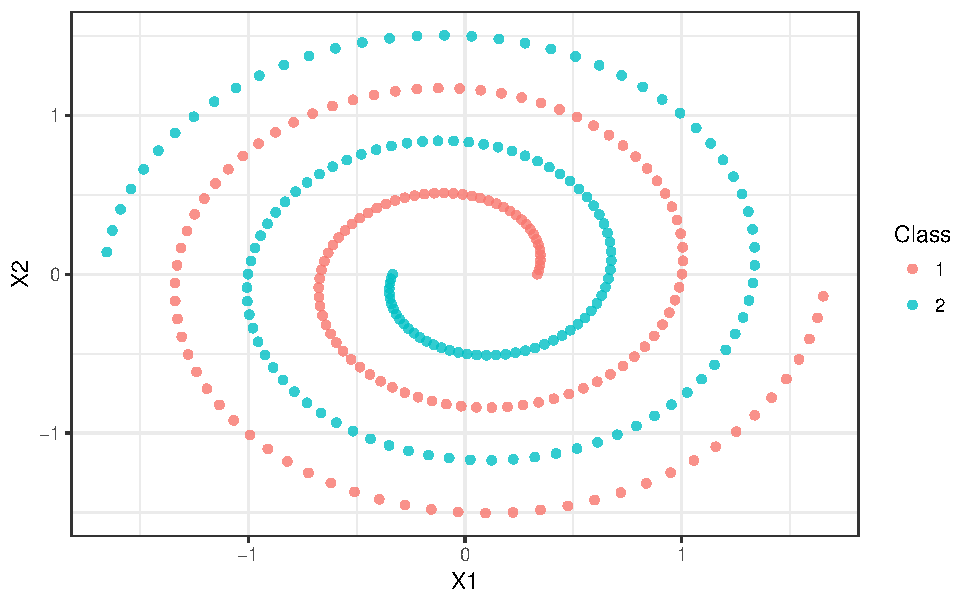
\includegraphics[width=0.7\textwidth]{figure/05-example_data}
  \caption{A scatter plot of simulated spiral data set.}
  \vspace{-0.5em}
  \label{fig:exampleiprobit}
\end{figure}

The three methods pretty much concur on the estimation of the intercept, but not on the RKHS scale parameter.
As a result, the log-density value calculated at the parameter estimates is also different in all three methods.
Notice the high posterior standard deviation for the scale parameter in the HMC method.
The posterior density for $\lambda$ was very positively skewed, and this contributed to the large posterior mean.

\begin{table}[hbt]
\centering
\caption{Table comparing the estimated parameter values, (marginal) log-likelihood values, and also time taken for the three estimation methods.}
\label{tab:compreiprobit}
\begin{tabular}{@{}lrrr@{}}
\toprule
& Laplace approximation 
& Variational EM 
& Hamiltonian MC          \\ \midrule
Intercept ($\alpha$)      & -0.02 (0.03)           & 0.00 (0.06)    & 0.00 (0.58)  \\
Scale ($\lambda$)      & 0.85 (0.01)         & 5.67 (0.23)  & 29.3 (5.21)     \\[0.5em]
Log-density    & -171.8              & -43.2       & -8.5                  \\
Error rate (\%) & 44.7               & 0.00        & 0.00                   \\
Brier score & 0.20               & 0.02        & 0.01                   \\[0.5em]
Iterations     & 20                  & 56          & 2000                    \\
Time taken (s) & >3600                & 5.32         & >1800                     \\ \bottomrule
\end{tabular}
\end{table}


\begin{figure}[p]
  \centering
  \vspace{1em}
  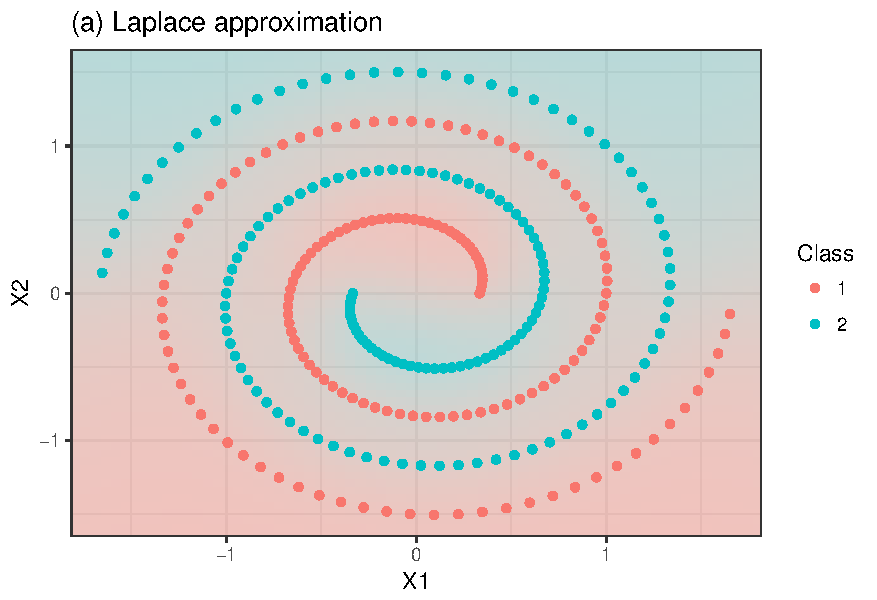
\includegraphics[width=0.49\textwidth]{figure/05-fit_lap}
  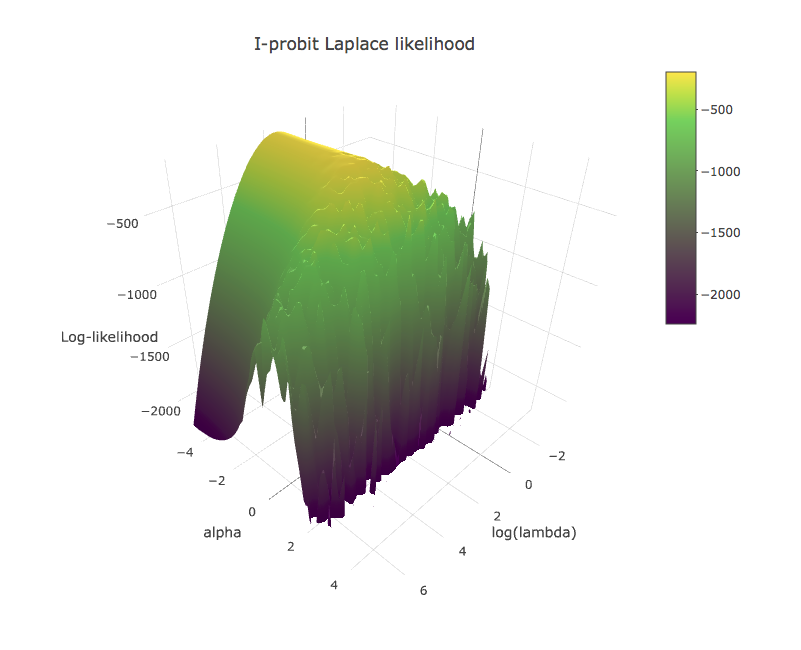
\includegraphics[width=0.49\textwidth]{figure/05-lik_lap}
  \vspace{1em}
  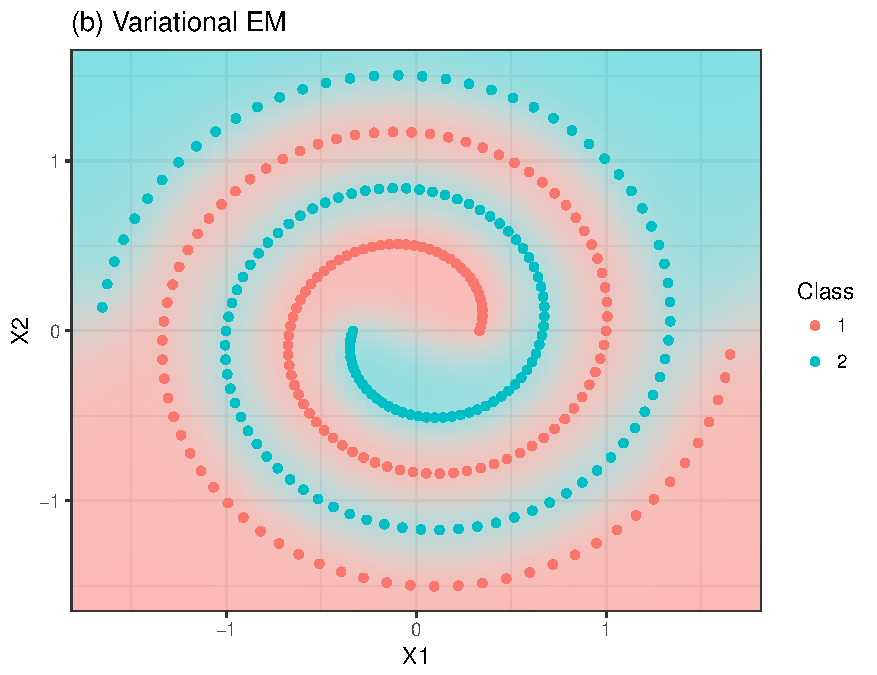
\includegraphics[width=0.49\textwidth]{figure/05-fit_vi}
  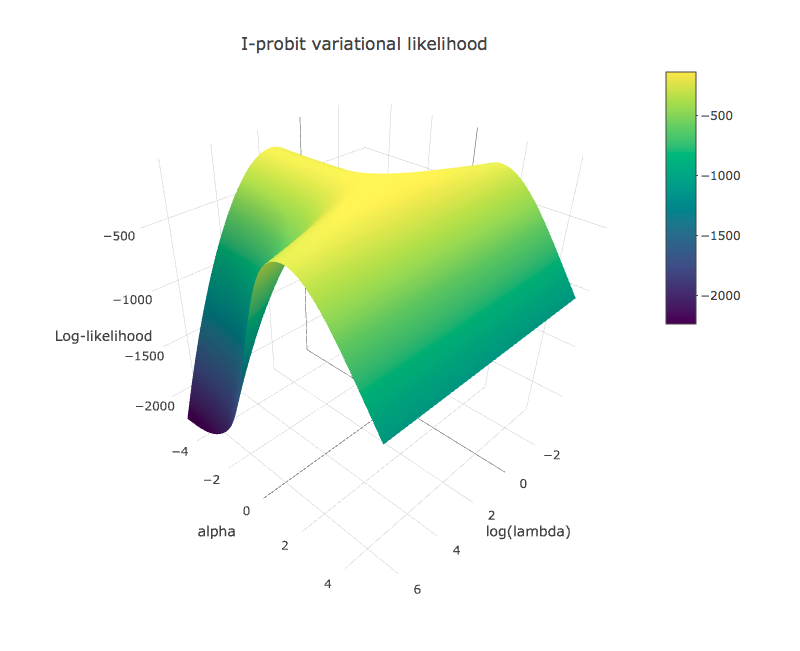
\includegraphics[width=0.49\textwidth]{figure/05-lik_vi}
  \vspace{1em}
  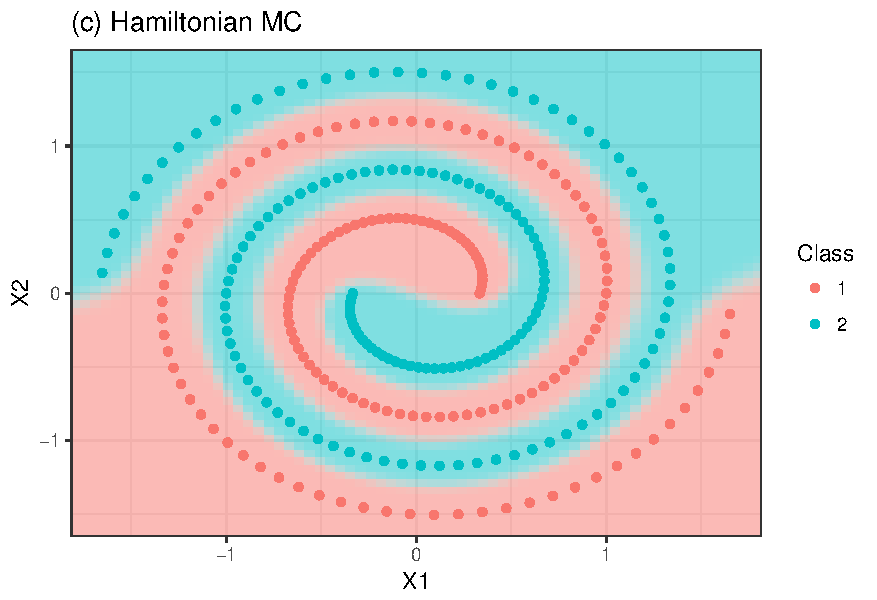
\includegraphics[width=0.49\textwidth]{figure/05-fit_hmc}
  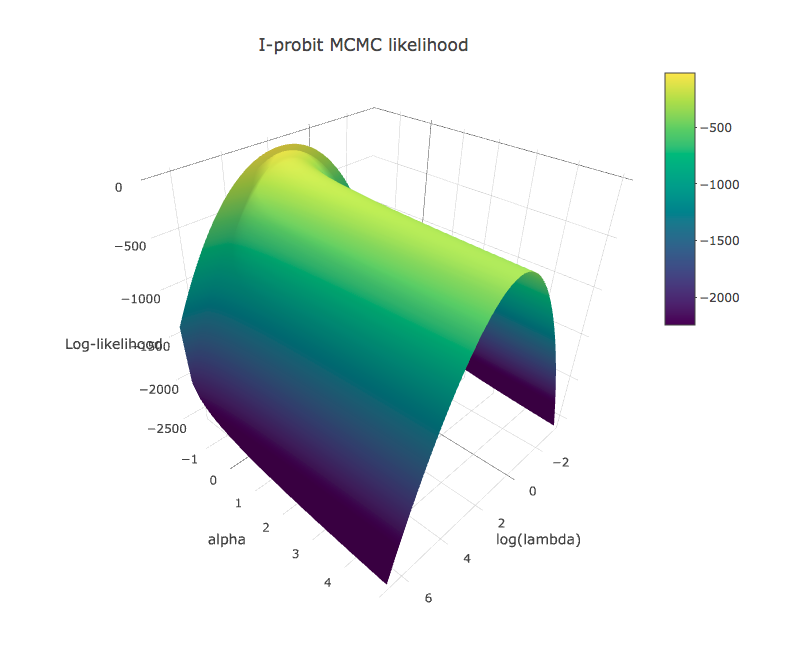
\includegraphics[width=0.49\textwidth]{figure/05-lik_hmc}
  \caption[Predicted probabilities and log-density plots]{Plots showing predicted probabilities (shaded region) for belonging to class `1' or `2' indicated by colour and intensity, and log-likelihood/ELBO surface plots for (a) Laplace's method, (b) variational EM, and (c) Hamiltonian MC. For the Hamiltonian MC plot, parameters are treated as fixed, and the mean log-density of the I-probit model recorded.}
  \label{fig:exampleiprobitfit}
\end{figure}
\index{Brier score}

\index{Laplace's method}
A plot of the log-likelihood (or ELBO) surface for three methods in \cref{fig:exampleiprobitfit} reveals some insight.
The variational likelihood has two ridges, with the maxima occurring around the intersection of these two ridges.
The Laplace likelihood seems to indicate a similar shape---in both the Laplace and variational method, the posterior distribution of $\bw$ is approximated by a Gaussian distribution, with different means and variances.
However, parts of the Laplace likelihood are poorly approximated resulting in a loss of fidelity around the supposed maxima, which might have contributed to the set of values that were estimated.
Laplace's method is known to yield poor approximations to probit model likelihoods \citep{kuss2005assessing}.
On the other hand, the log-likelihood calculated using a Hamiltonian MC sampler (treating parameters as fixed values) yields a slightly different graph: the log-likelihood increases as values of $\alpha$ become larger, resulting in the upwards inflection of the log-likelihood surface (as opposed to a downward inflection seen in the variational and Laplace likelihood).

In terms of predictive abilities, both the variational and Hamiltonian MC methods, even though the posteriors are differently estimated, have good predictive performance as indicated by their error rates and Brier scores\footnote{\index{Brier score}The Brier score is defined as $\frac{1}{n}\sum_{i=1}^n\sum_{j=1}^m (y_{ij} - \hat p_{ij})$ with $y_{ij}=1$ if $y_i = j$ and zero otherwise, and $\hat p_{ij}$ is the fitted probability $\hat\Prob(y_i = j)$. It gives a better sense of ``training/test error'', compared to simple misclassification rates, by accounting for the forecasted probabilities of the events happening. The Brier score is a proper scoring rule, i.e. it is uniquely minimised by the true probabilities.}.
\cref{fig:exampleiprobitfit} shows that HMC is more confident of new data predictions compared to variational inference, as indicated by the intensity of the shaded regions (HMC is shaded stronger than variational EM).
Laplace's method gave poor predictive performance.

Finally, on the computational side, variational inference was by far the fastest method to fit the model.
Sampling using Hamiltonian MC was very slow, because the parameter space is in effect $O(n + 2)$ (parameters are $\{w_1,\dots,w_n,\alpha,\lambda\}$ under the model with likelihood \cref{eq:intractablelikelihood2}, i.e. without the data augmentation scheme).
As for Laplace, each Newton step involves obtaining posterior modes of the $w_i$'s, and this contributed to the slowness of this method.
The reality is that variational inference takes seconds to complete what either the Laplace or full MCMC methods would take minutes or even hours to.
The predictive performance, while not as good as HMC, is certainly an acceptable compromise in favour of speed.
\vspace{-1em}


\section{A variational algorithm}\label{sec:iprobitvar}
%We present an EM algorithm to estimate the I-probit latent variables $\by^*$ and $\bw$, in which the E-step consists of a mean-field variational approximation of the conditional density $p(\by^*,\bw|\by,\theta) = q(\by^*)q(\bw)$.
As per assumptions $\ref{ass:A4}$, $\ref{ass:A5}$ and $\ref{ass:A6}$, the parameters of the I-probit model consists of $\theta =\{ \balpha = (\alpha_1,\dots,\alpha_m)^\top,\eta \}$.

The algorithm cycles through a variational inference E-step, in which the variational density $q(\by^*,\bw) = \prod_{i=1}^n q(\by^*_{i\bigcdot}) q(\bw)$ is optimised with respect to the Kullbeck-Leibler divergence $\KL\big[ q(\by^*,\bw) \Vert p(\by^*,\bw|\by) \big]$, and an M-step, in which the approximate expected joint density \cref{eq:iprobitQEstep} is maximised with respect to the parameters $\theta$. 
Convergence is assessed by monitoring the ELBO.
Apart from the fact that the variational EM algorithm uses approximate conditional distributions and involves matrices $\by^*$ and $\bw$, it is very similar to the EM described in \cref{chapter4}, and as such, the efficient computational work derived there is applicable.

\subsection{The variational E-step}

Let $\tilde q(\by^*,\bw)$ be the pdf that minimises the Kullbeck-Leibler divergence $\KL\big[ q \Vert p \big]$ subject to the mean-field constraint $q(\by^*,\bw) = q(\by^*)q(\bw)$.
By appealing to \citet[equation 10.9, p. 466]{bishop2006pattern}, the optimal mean-field variational density $\tilde q$ for the latent variables $\by^*$ and $\bw$ satisfy
\begin{align}
  \log \tilde q(\by^*) &= \E_{\bw\sim\tilde q} \big[ \log p(\by,\by^*,\bw) \big] + \const \\
  \log \tilde q(\bw) &= \E_{\by^*\sim\tilde q} \big[ \log p(\by,\by^*,\bw) \big] + \const 
\end{align}
where $p(\by,\by^*,\bw) = p(\by|\by^*) p(\by^*|\bw) p(\bw)$ is as per \cref{eq:iprobitlik}.
We now present the variational densities $\tilde q(\by^*)$ and $\tilde q(\bw)$.
For further details on the derivation of these densities, please refer to the appendix.

\subsubsection{Variational distribution for the latent propensities \texorpdfstring{$\by^*$}{$y^*$}}

The fact that the rows $\by_{i \bigcdot}^* \in \bbR^m$, $i=1,\dots,n$ of $\by^* \in \bbR^{n \times m}$ are independent can be exploited, and this results in a further induced factorisation $q(\by^*) = \prod_{i=1}^n q(\by_i^*)$.
Define the set $\cC_j = \{y_{ij}^* > y_{ik}^* \,|\, \forall k\neq j \}$.
Then $q(\by_{i \bigcdot}^*)$ is the density of a multivariate normal distribution with mean $\tilde \bmu_{i \bigcdot} = \balpha + \tilde\bw^\top  \bh_\eta(x_i)$, where $\tilde \bw = \E_{\bw\sim\tilde q}\bw$, and variance $\bPsi^{-1}$, subject to a truncation of its components to the set $\cC_{y_i}$.
That is, for each $i=1,\dots,n$ and noting the observed categorical response $y_i \in \{1,\dots,m\}$ for the $i$'th observation, the $\by_i^*$'s are distributed according to
\begin{align}\label{eq:ystardist}
  \by_{i \bigcdot}^* \iid
  \begin{cases}
    \N_m(\tilde\bmu_{i \bigcdot},  \bPsi^{-1}) & \text{ if } y_{iy_i}^* > y_{ik}^*, \forall k \neq y_i \\
    0 & \text{ otherwise}. \\
  \end{cases}
\end{align}
We denote this by $\by_{i \bigcdot}^* \iid \tN(\tilde\bmu_{i \bigcdot}, \bPsi^{-1},\cC_{y_i})$, and the important properties of this distribution are explored in the appendix.

The required expectation $\tilde\by^* := \E_{\by^*\sim\tilde q}\by^*_{i\bigcdot} = \E_{\by^*\sim\tilde q} (y_{i1}^*,\dots, y_{im}^*)^\top$ in the M-step can be tricky to obtain.
One strategy that can be considered is Monte Carlo integration: using samples from $\N_m(\tilde\bmu_{i \bigcdot},  \bPsi^{-1})$, disregard those that do not satisfy the condition $y_{iy_i}^* > y_{ik}^*, \forall k \neq j$, and then take the sample average.
This works reasonably well so long as the truncation region does not fall into the extreme tails of the multivariate normal.
Alternatively, a fast, Gibbs-based approach \citep{robert1995simulation} for sampling from a truncated multivariate normal can be implemented, and this is detailed in the appendix.

If the independent I-probit model is under consideration, whereby the covariance matrix has the independent structure $\bPsi = \diag(\sigma_1^{-2},\dots,\sigma_m^{-2})$, then the first moment  can be considered component-wise. 
Each component of this expectation is given by
\begin{align}\label{eq:ystarupdate}
  \tilde y_{ik}^* =
  \begin{cases}
    \tilde\mu_{ik} - \sigma_k C_i^{-1} \displaystyle{  \int \phi_{ik}(z) \prod_{l \neq k,y_i} \Phi_{il}(z) \phi(z) \dint z }
    &\text{ if } k \neq y_i \\[1.5em]
    \tilde\mu_{iy_i} - \sigma_{y_i} \sum_{k \neq y_i} \big(\tilde y_{ik}^* -  \tilde\mu_{ik} \big) 
    &\text{ if } k = y_i \\
  \end{cases}
\end{align}
with 
\begin{align*}
  \phi_{ik}(Z) &= \phi \left(\frac{\sigma_{y_i}}{\sigma_k} Z + \frac{\tilde\mu_{iy_i} - \tilde\mu_{ik}}{\sigma_k} \right) \\
  \Phi_{ik}(Z) &= \Phi \left(\frac{\sigma_{y_i}}{\sigma_k} Z + \frac{\tilde\mu_{iy_i} - \tilde\mu_{ik}}{\sigma_k} \right) \\
  C_i &= \int \prod_{l \neq j} \Phi_{il}(z) \phi(z) \dint z
\end{align*}
and $Z \sim \N(0,1)$ with pdf and cdf $\phi(\cdot)$ and $\Phi(\cdot)$ respectively. 
The integrals that appear above are functions of a unidimensional Gaussian pdf, and these can be computed rather efficiently using quadrature methods.

\subsubsection{Variational distribution for the I-prior random effects \texorpdfstring{$\bw$}{$w$}}

Given that both $\vecc \by^* | \vecc \bw$ and $\vecc\bw$ are normally distributed as per the model \cref{eq:iprobitmod}, we find that the full conditional distribution $p(\bw|\by^*,\by) \propto p(\by^*,\by,\bw) \propto p(\by^*|\bw)p(\bw)$ is also normal. 
The variational density $q$ for $\vecc \bw \in \bbR^{nm}$ is found to be Gaussian with mean and precision given by
\begin{gather}\label{eq:varipostw}
   \vecc \tilde\bw = \tilde\bV_w 
    (\bPsi \otimes \bH_\eta) \vecc (\tilde\by^* - \bone_n\balpha^\top)
  \hspace{0.5cm}\text{and}\hspace{0.5cm} 
  \tilde \bV_w^{-1} = \bPsi \otimes \bH_\eta^2 + \bPsi^{-1} \otimes \bI_n = \bV_{y^*}.
\end{gather}
As a computational remark, computing the inverse $\tilde\bV_w^{-1}$ presents a challenge, as this takes $O(n^3m^3)$ time if computed naïvely. 
By exploiting the Kronecker product structure in $\tilde\bV_w$, we are able to efficiently compute the required inverse in roughly $O(n^3m)$ time---see the \hltodo{Section X} for details.
Storage requirement is $O(n^2m^2)$, as a result of the covariance matrix in \cref{eq:varipostw}.

If the independent I-probit model is assumed, i.e. $\bPsi = \diag(\psi_1,\dots,\psi_m)$, then the posterior covariance matrix $\tilde\bV_w$ has a simpler structure which implies column independence in the matrix $\bw$.
By writing $\bw_{\bigcdot j} = (w_{1j},\dots,w_{nj})^\top \in \bbR^n$, $j=1,\dots,m$, to denote the column vectors of $\bw$, and with a slight abuse of notation, we have that
\begin{align*}
  \N_{nm}(\vecc \bw|\vecc\wtilde, \tilde\bV_w) 
  = \prod_{j=1}^m \N_{n}(\bw_{\bigcdot j}|\tilde\bw_{\bigcdot j}, \tilde\bV_{w_j}),
\end{align*}
where 
\[
  \tilde \bw_{\bigcdot j} = \psi_j\tilde \bV_{w_j}\bH_\eta (\tilde\by^*_j - \alpha_j\bone_n) \ \text{ and } \ \tilde \bV_{w_j} = \big(\psi_j\bH_{\eta}^2 + \psi_j^{-1}\bI_n \big)^{-1}.
\]
We note the similarity between \cref{eq:varipostw} above and the posterior distribution for the I-prior random effects in a normal model \cref{eq:posteriorw} seen in the previous chapter, with the difference being \cref{eq:varipostw} uses the continuous latent propensities $\by^*$ instead of the the observations $\by$.
The consequence of this is that the posterior regression functions are class independent, the exact intended effect by specifying a diagonal precision matrix $\bPsi$.
Storage requirement is $O(n^2m)$, since we need $\bV_{w_1},\dots,\bV_{w_m}$.

\begin{remark}
  The variational distribution $q(\bw)$ which approximates $p(\bw|\by)$ is in fact exactly $p(\bw|\by^*)$, the conditional density of the I-prior random effects given the latent propensities.
  By the law of total expectations, 
  \begin{gather*}
    \E[r(\bw)|\by] = \E_{\by^*}\big[ \E[r(\bw)|\by^*] \,|\, \by \big],
  \end{gather*}
  where $r(\cdot)$ is some function of $\bw$, and expectations are taken under the posterior distribution of $\by^*$.
  Hypothetically, if the true pdf $p(\by^*|\by)$ were tractable,  then the E-step can be computed using the true conditional distribution.
  Since it is not tractable, we resort to an approximation, and in the case of a variational approximation, \cref{eq:varipostw} is obtained.
\end{remark}



\subsection{The M-step}
\label{sec:varupdeta}

From \cref{eq:iprobitQEstep}, the function to be maximised in the M-step is
\begin{align*}
  Q(\theta) 
  &=\const -\half\tr\Big( \bPsi\E[\bw^\top\bH_\eta^2\bw]  + \bPsi^{-1} \E[\bw^\top\bw] \Big)   \\
  &\phantom{==} - \half \tr \Big( 
  \bPsi \Big( 
  \E[\by^{*\top}\by^*]
  + n \balpha\balpha^\top 
  - 2\tilde\by^{*\top}\bone_n \balpha^\top 
  - 2\tilde\bw^\top\bH_\eta (\tilde\by^* - \bone_n\balpha^\top) 
  \Big) \Big) \tag{\ref{eq:iprobitQEstep}}
  ,
\end{align*}
where expectations are taken with respect to the variational distributions of $\by^*$ and $\bw$. 
Note that since $\bPsi$ is treated as fixed, the term $\E[\by^{*\top}\by^*]$ is absorbed into the constant.
On closer inspection, the trace involving the second moments of $\bw$ is found to be
\begin{align*}
  \tr \Big( \bPsi\E[\bw^\top\bH_\eta^2\bw]  + \bPsi^{-1} \E[\bw^\top\bw] \Big)
  &= \sum_{i,j=1}^m \left\{ \psi_{ij} \tr(\bH_\eta^2\tilde\bW_{ij}) + \psi_{ij}^- \tr(\tilde\bW_{ij}) \right\}
\end{align*}
by the results of \hltodo{equation} derived in the appendix.
In the above, we had defined $\psi_{ij}^-$ to be the $(i,j)$'th element of $\bPsi^{-1}$, and
\[
  \tilde\bW_{ij} 
  = \E[\bw_{\bigcdot i}\bw_{\bigcdot j}^\top]
  =  \bV_{w}[i,j] + \tilde\bw_{\bigcdot i} \tilde\bw_{\bigcdot j}^\top,
\]
where $\bV_{w}[i,j] \in \bbR^{n\times n}$ refers to the $(i,j)$'th submatrix block of $\bV_w$, and the $n$-vector $\tilde \bw_{\bigcdot j} = \big(\E [w_{ij}] \big)_{i=1}^n$ is the expected value of the random effects for class $j$.
Specifically, when the error precision is of the form $\bPsi = \diag(\psi_1,\dots,\psi_m)$, this trace reduces to
\begin{align*}
  \tr \Big( \bPsi\E[\bw^\top\bH_\eta^2\bw]  + \bPsi^{-1} \E[\bw^\top\bw] \Big)
  &= \sum_{j=1}^m \left\{ \psi_j \tr(\bH_\eta^2\tilde\bW_{jj}) + \psi_j^{-1} \tr(\tilde\bW_{jj}) \right\} \\
  &= \sum_{j=1}^m \tr\big( 
  (\greyoverbrace{\psi_j\bH_\eta^2 + \psi_j^{-1}\bI_n}{\bSigma_{\theta,j}}) 
  \tilde\bW_{jj} \big)
\end{align*}

The bulk of the computational effort required to evaluate $Q(\theta)$ stems from the trace involving the second moments of $\bw$, and the fact that $\bH_\eta^2$ needs to be reevaluated each time $\theta = \{\balpha,\eta\}$ changes.
As discussed previously, each E-step takes $O(n^3m)$ time to compute the required first and second (approximate) posterior moments of $\bw$.
Once this is done, we can use the `front-loading of the kernel matrices' trick described in \cref{sec:efficientEM1}, which effectively renders the evaluation of $Q$ to be linear in $\theta$ (after an initial $O(n^2)$ procedure at the beginning).

As in the normal linear model, we employ a sequential update of the parameters (à la expectation conditional maximisation algorithm) by solving the first order conditions
\begin{align}
  \frac{\partial}{\partial\eta}Q(\eta|\balpha)
  &= -\half \sum_{i,j=1}^m \psi_{ij} \tr \left( \frac{\partial \bH_\eta^2}{\partial\eta} \tilde\bW_{ij} \right) 
  + \tr\left( \bPsi \tilde\bw^\top  \frac{\partial \bH_\eta}{\partial\eta} (\tilde\by^* - \bone_n\balpha^\top)  \right) \label{eq:vemeta} \\
  \frac{\partial}{\partial\balpha}Q(\balpha|\eta)
  &= 2n\bPsi\balpha - 2 \sum_{i=1}^n \bPsi \big(\by_{i\bigcdot}^* - \tilde\bw^\top\bh_\eta(x_i) \big) \label{eq:vemalpha}
\end{align}
equated to zero, where $\bh_\eta(x_i) \in \bbR^n$ is the $i$'th row of the kernel matrix $\bH_\eta$.
We now present the update equations for the parameters.

\subsubsection{Update for kernel parameters $\eta$}

When only ANOVA RKHS scale parameters are involved, then the conditional solution of $\eta$ to \cref{eq:vemeta} can be found in closed-form, much like in the exponential family EM algorithm described in \cref{sec:expfamEM}.
Under the same setting as in that subsection, assume that only $\eta = \{\lambda_1,\dots,\lambda_p\}$ need be estimated, and for each $k=1,\dots,p$, we can decompose the kernel matrix as $\bH_\eta = \lambda_k \bR_k + \bS_k$ and its square as $\bH_\eta^2 = \lambda_k^2 \bR_k^2 + \lambda_k \bU_k + \bS_k^2$.
As a follow-on from \cref{eq:vemeta}, the conditional solution for $\lambda_k$ given the rest of the parameters is obtained by solving
\begin{align*}
  \frac{\partial}{\partial\lambda_k}Q(\lambda_k|\balpha,\blambda_{-k})
  &= -\half \sum_{i,j=1}^m \psi_{ij} \tr \left( (2\lambda_k\bR_k^2 + \bU_k) \tilde\bW_{ij} \right) 
  + \tr\left( \bPsi \tilde\bw^\top \bR_k (\tilde\by^* - \bone_n\balpha^\top)  \right) \\
  &= - \lambda_k \sum_{i,j=1}^m \psi_{ij} \tr(\bR_k^2\tilde\bW_{ij})
  - \half \sum_{i,j=1}^m \psi_{ij} \tr(\bU_k\tilde\bW_{ij}) \\
  &\phantom{==} + \tr\left( \bPsi \tilde\bw^\top \bR_k (\tilde\by^* - \bone_n\balpha^\top)  \right) \\
  &=0.
\end{align*}
This yields the solution
\[
  \hat\lambda_k 
  = \frac{
  \tr\left( \bPsi \tilde\bw^\top \bR_k (\tilde\by^* - \bone_n\balpha^\top) \right)
  - \half \sum_{i,j=1}^m \psi_{ij} \tr(\bU_k\tilde\bW_{ij})
  }{
  \sum_{i,j=1}^m \psi_{ij} \tr(\bR_k^2\tilde\bW_{ij})
  }
\]
In the case of the independent I-probit model, where $\bPsi = \diag(\psi_1,\dots,\psi_m)$, $\hat\lambda_k$ has the form
\[
  \hat\lambda_k
  = \frac{
  \sum_{j=1}^m \psi_j \left( \tilde\bw^\top_{\bigcdot j} \bR_k (\tilde\by^*_{\bigcdot j} - \alpha_j\bone_n) - \half \tr(\bU_k\tilde\bW_{jj})\right)
  }{
  \sum_{j=1}^m \psi_j \tr(\bR_k^2\tilde\bW_{jj})
  }.
\]

\begin{remark}
  There is no closed-form solution for $\eta$ when the polynomial kernel is used, or when there are kernel parameters to optimise (e.g. Hurst coefficient or SE kernel lengthscale).
  In these situations, solutions for $\eta$ are obtained using numerical methods (i.e. employ quasi-Newton methods such as L-BFGS algorithm for optimising $Q(\eta|\balpha)$).
\end{remark}

\subsubsection{Update for intercepts \texorpdfstring{$\balpha$}{$\alpha$}}

It is easy to see that the unique solution to \cref{eq:vemalpha} is
\begin{align*}
  \hat\balpha
  &= \frac{1}{n} \bPsi^{-1} \left( \sum_{i=1}^n \bPsi \big(\by_{i\bigcdot}^* - \tilde\bw^\top\bh_\eta(x_i) \big) \right) 
  =\frac{1}{n} \sum_{i=1}^n \big(\by_{i\bigcdot}^* - \tilde\bw^\top\bh_\eta(x_i) \big) \in \bbR^m.
\end{align*}
Being free of $\bPsi$, the solution is the same whether the full or independent I-probit model is assumed.
Furthermore, we must have that $\sum_{j=1}^m \alpha_j = 0$ for identifiability, so as an additional step to satisfy this condition, the solution $\balpha$ is centred.

\subsection{Summary}

A summary of the variational EM algorithm is presented.
Notice that the evaluation of each component of the posterior depends on knowing the posterior distribution of the other, i.e. $q(\by^*)$ depends on $q(\bw)$ and vice-versa.
Similarly, each parameter update is obtained conditional upon the value of the rest of the parameters.
These circular dependencies are dealt with by way of an iterative updating scheme: with arbitrary starting values for the distributions $q^{(0)}(\by^*)$ and $q^{(0)}(\bw)$, and for the parameters $\theta^{(0)}$, each are updated in turn according to the above derivations.

The updating sequence is repeated until no significant increase in the convergence criterion, the ELBO, is observed.
The ELBO for the I-probit model is given by the quantity
\begin{align}
  \cL_q(\theta) = \half[nm] + \sum_{i=1}^n \log C_i(\theta) + \half\log \abs{\tilde\bV_w} - \half[n]\log\abs{\bPsi} - \half\sum_{i,j=1}^m \psi_{ij}^- \tr(\tilde\bW_{ij}),
\end{align}
where $C_i(\theta)$ is the normalising constant of the distribution $\tN_m(\balpha + \bw^\top\bh_\eta(x_i),\bPsi^{-1},\cC_{y_i})$, with $\cC_{y_i} = \{y_{iy_i}^* > y_{ik}^* | \forall k \neq y_i \}$.
That is,
\[
  C_i(\theta) = \idotsint\displaylimits_{\{y_{iy_i}^* > y_{ik}^* | \forall k \neq y_i \}} \phi(y_{i1}^*, \dots, y_{im}^*|\balpha + \bw^\top\bh_\eta(x_i), \bPsi^{-1}) \dint y_{i1}^* \cdots \dint y_{im}^*.
\]
Similar to the EM algorithm, each iteration of the algorithm increases the ELBO to a stationary point \citep{blei2017variational}.
Unlike the EM algorithm though, the variational EM algorithm does \emph{not} guarantee an increase in the marginal log-likelihood at each step, nor does it guarantee convergence to the global maxima of the log-likelihood.

Further, the ELBO expression to be maximised is often not convex, which means the CAVI algorithm may terminate at local modes, for which they may be many.
Note that the variational distribution with the higher ELBO value is the distribution that is closer, in terms of the KL divergence, to the true posterior distribution.
In our experience, multiple random starts alleviates this issue for the I-probit model.

\algrenewcommand{\algorithmiccomment}[1]{{\color{gray} \hfill $\triangleright$ #1}}
\begin{algorithm}[p]
\caption{Variational EM for the I-probit model (fixed $\bPsi$)}\label{alg:varemiprobit}
\begin{algorithmic}[1]
  \Procedure{Initialisation}{}
    \State Initialise $\theta^{(0)} \gets \{\balpha^{(0)},\eta^{(0)}\}$
    \State $\tilde q^{(0)}(\bw) \gets \MN(\bzero,\bI_n,\bPsi)$
    \State $\tilde q^{(0)}(\by^*_{i\bigcdot}) \gets \tN_m(\tilde\balpha^{(0)},\bPsi^{-1},\cC_{y_i})$
    \State $t \gets 0$
  \EndProcedure 
  \Statex
  \While{not converged}{}
    \Procedure{Variational E-step}{}
      \For{$i=1,\dots,n$} \Comment{Update $\by^*$}
        \State $\tilde q^{(t+1)}(\by^*_{i \bigcdot}) \gets \tN_m\big(\tilde\balpha^{(t)} + \tilde\bw^{(t)\top} \bh_{\eta^{(t)}}(x_i), \bPsi, \cC_{y_i}\big)$ 
        \State $\tilde \by^{*(t+1)}_{i \bigcdot} \gets \E_{q^{(t+1)}}[\by^*_{i \bigcdot}]$
      \EndFor
      \Statex
      \State $\tilde\bV_w^{(t+1)} \gets \big((\bPsi \otimes \bH_{\eta^{(t)}}^2) + (\bPsi^{-1} \otimes \bI_n)\big)^{-1}$ \Comment{Update $\bw$}
      \State $\vecc\tilde\bw^{(t+1)}  \gets \tilde\bV_w^{(t+1)} 
      (\bPsi \otimes \bH_{\eta^{(t)}}) \vecc (\tilde\by^{*(t+1)} - \bone_n\balpha^{(t)\top})$
      \State $\tilde q^{(t+1)}(\bw) \gets \N_{nm}\big( \vecc \tilde\bw^{(t+1)}, \tilde\bV_w^{(t+1)} \big)$ 
    \EndProcedure
    \Statex
    \Procedure{M-step}{}
      \If{ANOVA kernel (closed-form updates)} \Comment{Update $\eta$}
        \For{$k=1,\dots,p$} 
          \State $T_{1k} \gets \sum_{i,j=1}^m \psi_{ij} \tr(\bR_k^2\tilde\bW_{ij})$ 
          \State $T_{2k} \gets \tr\left( \bPsi \tilde\bw^\top \bR_k (\tilde\by^* - \bone_n\balpha^\top) \right) - \half \sum_{i,j=1}^m \psi_{ij} \tr(\bU_k\tilde\bW_{ij})$ 
          \State $\lambda_k^{(t+1)} \gets T_{2k}/T_{1k}$           
        \EndFor
      \Else
        \State $\eta^{(t+1)} \gets \argmax_\eta Q(\eta|\balpha^{(t)})$ by L-BFGS algorithm
      \EndIf
      \Statex
      \State $\ba \gets \frac{1}{n} \sum_{i=1}^n \big( \tilde\by^{*(t+1)}_{i \bigcdot} - \tilde\bw^{(t+1)\top} \tilde\bh_{\eta^{(t+1)}}(x_i) \big)$ \Comment{Update $\balpha$}
      \State $\balpha^{(t+1)} \gets \ba - \frac{1}{m}\sum_{j=1}^m a_j$
    \EndProcedure
    \Statex
    \State Calculate ELBO $\cL^{(t+1)}$
    \State $t \gets t + 1$
  \EndWhile
\end{algorithmic}
\end{algorithm}


\section{Post-estimation}
%\index{I-probit!posterior distribution}
Post-estimation procedures such as obtaining predictions for a new data point, the credibility interval for such predictions, and model comparison, are of interest.
These are performed in an empirical Bayes manner using the variational posterior density of the regression function obtained from the output of the variational EM algorithm.

We first describe prediction of a new data point $x_{\text{new}}$.
Step one is to determine the distribution of the posterior regression functions in each class, $\bff(x_{\text{new}}) = \bw^\top\bh_\eta(x_{\text{new}})$, where $\bh_\eta(x_{\text{new}})$ is the vector of length $n$ containing entries $h_\eta(x_i,x_\new)$, given values for the parameters $\theta$ of the I-probit model.
To this end, we use the ELBO estimates for $\theta$, i.e. $\hat\theta = \argmax_\theta \cL_q(\theta)$, as obtained from the variational EM algorithm.
As we know, the variational distribution of $\vecc\bw$ is normally distributed with mean and variance according to \cref{eq:varipostw}.
By writing $\vecc \tilde\bw = (\tilde \bw_{\bigcdot 1}, \dots, \tilde \bw_{\bigcdot m})^\top$ to separate out the I-prior random effects per class, we have that $\bw_{\bigcdot j}|\hat\theta \sim \N_n(\tilde \bw_{\bigcdot j}, \tilde\bV_w[j,j])$, and $\Cov(\bw_{\bigcdot j},\bw_{\bigcdot k}) = \tilde\bV_w[j,k]$, where the `$[\cdot,\cdot]$' indexes the $n\times n$ sub-block of the block matrix $\bV_w$.
Thus, for each class $j=1,\dots,m$ and any $x \in \cX$,
\[
  f_j(x)|\by,\hat\theta \sim \N\Big(\,
  \bh_{\hat\eta}(x)^\top \tilde\bw_{\bigcdot j} \, , \,
  \bh_{\hat\eta}(x)^\top\tilde\bV_w[j,j] \, \bh_{\hat\eta}(x)
  \Big),
\]
and the covariance between the regression functions in two different classes is
\[
  \Cov\big(f_j(x),f_k(x)|\by,\hat\theta \big) = 
  \bh_{\hat\eta}(x)^\top \tilde\bV_w[j,k] \, \tilde\bh_{\hat\eta}(x).
\]
\index{I-probit!posterior predictive distribution}Then, in step two, using the results obtained in the previous chapter in \cref{sec:ipriorpostest} \colp{\mypageref{sec:ipriorpostest}}, we have that the latent propensities $y_{\new,j}^*$ for each class are normally distributed with mean, variance, and covariances
\begin{alignat*}{3}
  \E(y_{\new,j}^*|\by,\hat\theta) 
  &= \hat\alpha_j + \E \big( f_j(x_\new) |\by,\hat\theta \big)
  &&=: \hat\mu_j(x_\text{new}) \\
  \Var(y_{\new,j}^*|\by,\hat\theta) 
  &= \Var\big(f(x_\new)|\by,\hat\theta \big) + \bPsi^{-1}_{jj}
  &&=: \hat\sigma_j^2(x_\text{new}) \\
  \Cov(y_{\new,j}^*,y_{\new,k}^*|\by,\hat\theta)
  &= \Cov\big(f_j(x),f_k(x)|\by,\hat\theta \big) + \bPsi^{-1}_{jk}
  &&=: \hat\sigma_{jk}(x_\text{new}).
\end{alignat*}

From here, step three would be to extract class information of data point $x_\text{new}$, which are contained in the normal distribution $\N_{m}\big(\hat\bmu_\new, \hat\bV_\new \big)$, where
\begin{equation*}
  \hat\bmu_\new = \big(\mu_1(x_\text{new}),\dots, \mu_m(x_\text{new}) \big)^\top 
  \hspace{0.5cm}\text{and}\hspace{0.5cm}
  \hat\bV_{\new,jk} = 
  \begin{cases}
    \hat\sigma_j^2(x_\text{new}) & \text{if } j = k \\
    \hat\sigma_{jk}(x_\text{new}) & \text{if } j \neq k. \\
  \end{cases}
\end{equation*}
The predicted class is inferred from the latent variables using
\[
  \hat y_{\text{new}} = \argmax_k \hat\mu_k(x_\new), 
\]
while the probabilities for each class are obtained by way of integration of a multivariate normal density, as per \cref{eq:pij}:
\begin{align}
  \hat p_{\text{new},j} 
  &=  \idotsint\displaylimits_{\{y^*_j > y^*_k | \forall k \neq j \}} \phi(y_{1}^*, \dots, y_{m}^*|\hat\bmu_\new, \hat\bV_{\new}) \dint y_{1}^* \cdots \dint y_{m}^*.
\end{align}
For the independent I-probit model, class probabilities are obtained in a more compact manner via
\[
  \hat p_{\text{new},j} 
  = \E_Z \Bigg[ \mathop{\prod_{k=1}^m}_{k\neq j} 
  \Phi \left(\frac{\hat\sigma_j(x_\text{new})}{\hat\sigma_k(x_\text{new})} Z + \frac{\hat\mu_j(x_\new) - \hat\mu_k(x_\new)}{\hat\sigma_k^2(x_\text{new})} \right) \Bigg],
\]
as per \cref{eq:pij2}, since the $m$ components of $\bff(x_\new)$, and hence the $\by^*_{\new,j}$'s, are independent of each other ($\bPsi$ and $\hat\bV_\new$ are diagonal).
Prediction of a single new data point takes $O(n^2m)$ time, because there are essentially $m$ I-prior posterior regression functions, and each take $O(n^2)$ to evaluate.
This is assuming negligible time to compute the class probabilities.

\index{credibility interval}
We are able to take advantage of the Bayesian machinery to obtain credibility intervals for probability estimates or any transformation of these probabilities (e.g. log odds or odds ratios).
The procedure is as follows.
First, obtain samples $\bw^{(1)},\dots,\bw^{(T)}$ by drawing from its variational posterior distribution $\vecc\bw^{(t)}|\hat\theta \sim \N_{nm}(\vecc \tilde\bw,\bV_w)$.
Then, obtain samples of class probabilities $\{p_{xj}^{(1)},\dots, p_{xj}^{(T)} \}_{j=1}^m$, for a given data point $x\in\cX$ by evaluating
\[
  p_{xj}^{(t)} = \idotsint\displaylimits_{\{y^*_j > y^*_k | \forall k \neq j \}} \phi\big(y_{1}^*, \dots, y_{m}^*|\hat\bmu^{(t)}(x), \hat\bV(x)\big) \dint y_{1}^* \cdots \dint y_{m}^*,
\]
where $\hat\bmu^{(t)}(x) = \hat\balpha + \bw^{(t)\top}\bh_{\hat\eta}(x)$, and $\hat\bV(x)_{jk}$ equals $\hat\sigma^2_j(x)$ if $j = k$, and $\hat\sigma_{jk}(x)$ otherwise.
To obtain a statistic of interest, say, a 95\% credibility interval of a function $r(p_{xj})$ of the probabilities, simply take the empirical lower 2.5th and upper 97.5th percentile of the transformed sample $\big\{ r(p_{xj}^{(1)}),\dots, r(p_{xj}^{(T)}) \big\}$.
%In this manner, all aspects of uncertainty, from the parameters to the latent variables of the generative model, are accounted for.

\begin{remark}
  \index{bootstrap}
  \index{variational EM algorithm!standard error}
  \index{standard error}
  Unfortunately, with the variational EM algorithm, standard errors for the parameters $\theta$ are not so easy to obtain.  
  We could not ascertain as to the availability of an unbiased estimate of the asymptotic covariance matrix for $\theta$ under a variational framework.
  One strategy for obtaining standard errors is bootstrap \citep{chen2017use}:
  \begin{enumerate}
    \item Obtain $\hat\theta = \argmax_\theta \cL_q(\theta)$ using $\cS = \{(y_1,x_1),\dots, (y_n,x_n)\}$.
    \item For $t=1,\dots,T$, do
    \begin{enumerate}
      \item Obtain $\cS^{(t)} = \{ (y_1^{(t)},x_1^{(t)}),\dots, (y_n^{(t)},x_n^{(t)})\}$ by sampling $n$ points with replacement from $\cS$.
      \item Compute $\hat\theta^{(t)} = \argmax_\theta \cL_q(\theta)$ using the data $\cS^{(t)}$.
    \end{enumerate}
    \item For the $l$'th component of $\theta$, compute its variance estimator using
    \[
      \widehat\Var(\hat\theta_l) = \frac{1}{T} \sum_{t=1}^T (\hat\theta_l^{(t)} - \bar\theta_l)^2
      \hspace{0.5cm}\text{where}\hspace{0.5cm}
      \bar\theta_l = \frac{1}{T} \sum_{t=1}^T \hat\theta_l^{(t)}.
    \]
%    where
%    \[
%      \bar\theta_l = \frac{1}{T} \sum_{t=1}^T \hat\theta_l^{(t)}.
%    \]
  \end{enumerate}
  The obvious potential downside to this bootstrapp scheme is computational time.
\end{remark}

\index{Bayes factor!empirical}
\index{empirical Bayes factor|see{Bayes factor}}
Finally, a discussion on model comparison, which, in the variational inference literature, is achieved by comparing ELBO values of competing models \citep{beal2003}.
The rationale is that the ELBO serves as a conservative estimate for the log marginal likelihood, which would allow model selection via (empirical) Bayes factors.
This stems from the fact that 
\begin{align*}
  \log p(\by|\theta) 
  &= \cL_q(\theta) + \KL(q \Vert p ) 
  > \cL_q(\theta),
\end{align*}
since the Kullback-Leibler divergence from the true posterior density $p(\by^*,\bw|\by)$ to the variational density $q(\by^*,\bw)$ is strictly positive (it is zero if and only if the two densities are equivalent), and is minimised under a variational inference scheme.
\citet{kass1995bayes} suggest \cref{tab:BF} as a way of interpreting  observed Bayes factor values $\BF(M_1,M_0)$ for comparing model $M_1$ against model $M_0$, where $\BF(M_1,M_0)$ is approximated by
\[
  \BF(M_1,M_0) \approx \frac{\cL_q(\theta|M_1)}{\cL_q(\theta|M_0)},
\]
and $\cL_q(\theta|M_k)$, $k=0,1$, is the ELBO for model $M_k$.
It should be noted that while this works in practice, there is no theoretical basis for model comparison using the ELBO \citep{blei2017variational}.

\index{Bayes factor}
\vspace{0.3em}
\begin{table}[htbp]\label{tab:BF}
  \centering
  \caption[Guidelines for interpreting Bayes factors]{Guidelines for interpreting Bayes factors \citep{kass1995bayes}.}
  \label{tab:bf}
  \begin{tabular}{lll}
    \toprule
    $2\log \BF(M_1,M_0)$ &$\BF(M_1,M_0)$ & Evidence against $M_0$ \\
    \midrule
    0--2  &1--3    &Not worth more than a bare mention \\ 
    2--6  &3--20   &Positive \\ 
    6--10 &20--150 &Strong \\ 
    >10   &>150    &Very strong \\ 
  \end{tabular}
\end{table}

\begin{remark}
  In the previous chapter on normal I-prior models, the I-prior could be integrated out of the model completely, resulting in a normal  log-likelihood for the parameters.
  Model comparison can be validly done using likelihood ratio tests and asymptotic chi-square distributions.
  Here however, we only have a lower bound to the log-likelihood, and most likely the asymptotic results of likelihood ratio tests do not hold.
  Then, the concept of approximate (empirical) Bayes factors seem most intuitive, even if not rooted in theory.
\end{remark}
\vspace{-1em}


\section{Computational consideration}
Computational challenges for the I-probit model stems from two sources: 1) calculation of the class probabilities \cref{eq:pij}; and 2) storage and time requirements for the variational EM algorithm.
Ways in which to overcome these challenges are discussed.
In addition, we also discuss considerations to take into account if estimation of the error precision $\bPsi$ is desired, and thus pave the way for future work.

\subsection{Efficient computation of class probabilities}
\label{sec:mnint}

The issue at hand here is that for $m>4$, the evaluation of the class probabilities in \cref{eq:pij} is computationally burdensome using classical methods such as quadrature methods \citet{geweke1994alternative}.
As such, simulation techniques (Monte Carlo integration) are employed instead.
The simplest strategy to overcome this is a frequency simulator (otherwise known as Monte Carlo integration): obtain random samples from $\N_{m}\big(\bmu(x_i), \bPsi^{-1}\big)$, and calculate how many of these samples fall within the required  region.
This method is fast and yields unbiased estimates of the class probabilities.
However, in an extensive comparative study of various probability simulators, \citet{hajivassiliou1996simulation} concluded that the Geweke-Hajivassiliou-Keane (GHK) probability simulator \citep{geweke1989bayesian,hajivassiliou1998method,keane1994solution} is the most reliable under a multitude of scenarios.
This is now described, and for clarity, we drop the subscript $i$ denoting individuals. 

Suppose that an observation $y=j$ has been made.
Reformulate $\by^*$ in \cref{eq:latentmodel} by anchoring on the $j$'th latent variable $y_j^*$ to obtain
\[
  \bz := (
  \myoverbrace{y_1^* - y_j^*}{ z_1},
  \dots,
  \myoverbrace{y_{j-1}^* - y_j^*}{ z_{j-1}},
  \myoverbrace{y_{j+1}^* - y_j^*}{ z_{j}},
  \dots, 
  \myoverbrace{y_m^* - y_j^*}{ z_{m-1}},
  )^\top \in \bbR^{m-1}.
\]
Note that we have indexed the vector $\bz$ using $j' = k$ if $k < j$, and $j' = k -1$ if $k > j$ for $k=1,\dots,m$, so that the index $j'$ runs from $1$ to $m-1$.
Let $\bQ \in \bbR^{(m-1)\times m}$ be a matrix formed by inserting a column of minus ones at the $j$'th position in an $(m-1)$ identity matrix.
We can then write $\bz = \bQ\by^*$, and thus we have that $\bz\sim\N_{m-1}(\bnu_{(j)}, \bOmega_{(j)})$, where $\bnu_{(j)} = \bQ\bmu(x_i)$ and $\bOmega_{(j)} = \bQ\bPsi^{-1}\bQ^\top$.
These are indexed by `$(j)$' because the transformation is dependent on which latent variable the $\bz$'s are anchored on.

\begin{remark}
  Incidentally, the probit model in \cref{eq:latentmodel} is equivalently represented by 
  \begin{equation}\label{eq:latentmodel2}
    y_i = 
    \begin{cases}
      1 & \text{if } \max (y_{i2}^* - y_{i1}^*,\dots,y_{im}^* - y_{i1}^*) < 0 \\
      j & \text{if } \max (y_{i2}^* - y_{i1}^*,\dots,y_{im}^* - y_{i1}^*) = y_{ij}^* - y_{i1}^* \geq 0,
    \end{cases}
  \end{equation}   
  which is obtained by anchoring on the first latent variable (referred to as the reference category), although the choice of reference category is arbitrary.
  This is similar to fixing the latent variables of the reference category to zero, and thus, as discussed previously in \cref{sec:iia}, full identification is achieved by fixing one more element of the covariance matrix.
\end{remark}

For the symmetric and positive definite covariance matrix $\bOmega_{(j)}$, obtain its Cholesky decomposition as $\bOmega_{(j)} = \bL\bL^\top$, where $\bL$ is a lower triangular matrix.
Then, $\bz = \bnu_{(j)} + \bL\bzeta$, where $\bzeta \sim\N_{m-1}(\bzero,\bI_{m-1})$.
That is,
\begin{align*}
  \begin{pmatrix}
    z_1 \\
    z_2 \\
    \vdots \\
    z_{m-1}
  \end{pmatrix}  
  &=
  \begin{pmatrix}
    \nu_{(j)1} \\
    \nu_{(j)2} \\    
    \vdots \\
    \nu_{(j)m-1}
  \end{pmatrix}  
  + 
  \begin{pmatrix}
    L_{11} &       &       & \\
    L_{21} &L_{22} &       & \\
    \vdots &\vdots &\ddots & \\
    L_{m-1,1} &L_{m-1,2} &\cdots &L_{m-1,m-1} \\
  \end{pmatrix} 
  \begin{pmatrix}
    \zeta_1 \\
    \zeta_2 \\    
    \vdots \\
    \zeta_{m-1}
  \end{pmatrix} \\ %\displaybreak
  &=
  \begin{pmatrix}
    \nu_{(j)1} + L_{11}\zeta_1 \\
    \nu_{(j)2} + \sum_{k=1}^2 L_{k2} \zeta_k \\    
    \vdots \\
    \nu_{(j)m-1} + \sum_{k=1}^{m-1} L_{k,m-1} \zeta_k
  \end{pmatrix}.  
\end{align*}

With this setup, the probability $p_{j}$ of an observation belonging to class $j$, which is equivalent to the probability that each $ z_{j'} < 0$, $j'=1,\dots,m-1$, can be expressed as
\begin{align*}
  p_j 
  ={}& \Prob( z_1 < 0,\dots, z_{m-1} < 0) \\
  ={}& 
  \Prob(\zeta_1 < u_1,\dots,\zeta_{m-1}<u_{m-1}) \\
  ={}& 
  \Prob(\zeta_1 < u_1)
  \Prob(\zeta_2 < u_2|\zeta_1 < u_1)
  \Prob(\zeta_3 < u_3|\zeta_1 < u_1,\zeta_2 < u_2)
  \cdots \\
  &\cdots
  \Prob(\zeta_{m-1}<u_{m-1}|\zeta_1 < u_1,\dots,\zeta_{m-2}<u_{m-2}),
\end{align*}
where 
\begin{equation*}
  u_{j'} = 
  u_{j'}(\zeta_1,\dots,\zeta_{j'-1}) =
  \begin{cases}
    - \nu_{(j)1} / L_{11} &\text{for } j' = 1 \\
    - \big(\nu_{(j)j'} + \sum_{k=1}^{j'-1} L_{kj'}\zeta_k \big) / L_{j'j'} &\text{for } j' = 2,\dots,m-1
  \end{cases}
\end{equation*}
The GHK algorithm entails making draws from one-sided right truncated standard normal distributions (for instance, using an inverse transform method detailed in \cref{apx:truncuninorm},  \mypageref{apx:truncuninorm}):
\begin{itemize}
  \item Draw $\tilde\zeta_1 \sim \tN(0,1,-\infty,u_1)$.
  \item Draw $\tilde\zeta_2 \sim \tN(0,1,-\infty,\tilde u_2)$, where $\tilde u_2 = u_2(\tilde\zeta_1)$.
  \item Draw $\tilde\zeta_3 \sim \tN(0,1,-\infty,\tilde u_3)$, where $\tilde u_3 = u_3(\tilde\zeta_1,\tilde\zeta_2)$. 
  \item $\cdots$
  \item Draw $\tilde\zeta_{m-1} \sim \tN(0,1,-\infty,\tilde u_{m-2})$, where $\tilde u_{m-1} = u_m(\tilde\zeta_1,\dots,\tilde\zeta_{m-2})$.
\end{itemize}
These values are then used in the following manner:
\begin{itemize}
  \item Use $\tilde\zeta_1$ to obtain a ``draw'' of $\Prob(\zeta_2 < u_2|\zeta_1 < \zeta_1)$,
  \begin{align*}
    \widetilde\Prob(\zeta_2 < u_2|\zeta_1 < \zeta_1)
    &=\Prob(\zeta_2 < u_2|\zeta_1 = \tilde\zeta_1) \\
    &= \Phi \Big( - \big(\nu_{(j)2} +  L_{12}\tilde\zeta_1 \big) / L_{22} \Big)
  \end{align*}
  \item Use $\tilde\zeta_1$ and $\tilde\zeta_2$ to obtain a ``draw'' of $\Prob(\zeta_3 < u_3|\zeta_1 < u_1,\zeta_2 < u_2)$,
  \begin{align*}
    \widetilde\Prob(\zeta_3 < u_3|\zeta_1 < u_1,\zeta_2 < u_2)
    &=\Prob(\zeta_3 < u_3|\zeta_1 = \tilde\zeta_1,\zeta_2 = \tilde\zeta_2)\\
    &= \Phi \Big( - \big(\nu_{(j)3} + L_{13}\tilde\zeta_1 + L_{23}\tilde\zeta_2 \big) / L_{33} \Big)
  \end{align*} 
  \item And so on. 
\end{itemize}
Therefore, a simulated probability for $p_j$ (denoted with a tilde) is obtained as
\begin{equation}\label{eq:tildepj}
  \tilde p_j = \Phi\left( -\nu_{(j)1}/ L_{11} \right) 
  \prod_{j'=2}^{m-1} \Phi \left( 
  - \big(\nu_{(j)j'} + \textstyle\sum_{k=1}^{j'-1} L_{kj'}\tilde\zeta_k \big) / L_{j'j'} 
  \right).
\end{equation}
By performing the above scheme $T$ number of times to obtain $T$ such simulated probabilities $\{p_j^{(1)},\dots,p_j^{(T)} \}$, the actual probability of interest $p_j$ is then approximated by the sample mean of the draws,
\[
  \hat p_j = \frac{1}{T} \sum_{t=1}^T p_j^{(t)}.
\]

If it so happens that one of the standard normal cdfs in \cref{eq:tildepj} is extremely small, this can cause loss of significance due to floating-point errors (catastrophic cancellation).
It is better to work on a log-probability scale, so the products in \cref{eq:tildepj} turn into sums, and revert back by exponentiating.

\begin{remark}
  The GHK algorithm provides reasonably fast and accurate calculations of class probabilities when $\bPsi$ is dense.
  As we alluded to earlier in the chapter, the class probabilities condense to a unidimensional integral involving products of normal cdfs (c.f. equation \ref{eq:pij2}) if $\bPsi$ is diagonal.
  Note that if $\bPsi$ is diagonal, then the transformed $\bOmega_{(j)} = \bQ\bPsi^{-1}\bQ^\top$ is certainly not: the components of $\bz$ are correlated because they are all anchored on the same random variable.
  Thus, direct evaluation of \cref{eq:pij2} using quadrature methods avoids the Cholesky step and random sampling employed by the GHK method.
\end{remark}

%\begin{remark}
%  The GHK probability simulator relates to the \emph{method of simulated likelihood}.  
%\end{remark}

\subsection{Efficient Kronecker product inverse}
\label{sec:complxiprobit}

As with the normal I-prior model, the time complexity of the variational inference algorithm for I-probit models is dominated by the step involving the posterior evaluation of the I-prior random effects $\bw$, which essentially is the inversion of an $nm \times nm$ matrix.
The matrix in question is %(from \cref{eq:varipostw})
\begin{align}
  \bV_w = \big[ (\bPsi \otimes \bH_\eta^2) + (\bPsi^{-1} \otimes \bI_n) \big]^{-1}. \tag{from \ref{eq:varipostw}}
\end{align}
We can actually exploit the Kronekcer product structure to compute the inverse efficiently.
Perform an orthogonal eigendecomposition of $\bH_\eta$ to obtain $\bH_\eta = \bV\bU\bV^\top$ and of $\bPsi$ to obtain $\bPsi = \bQ\bP\bQ^\top$.
This process takes $O(n^3 + m^3) \approx O(n^3)$ time if $m\ll n$ or if done in parallel, and needs to be performed once per CAVI iteration.
Then, manipulate $\bV_w^{-1}$ as follows:
\begin{align*}
  \bV_w^{-1} 
  &= (\bPsi \otimes \bH_\eta^2) + (\bPsi^{-1} \otimes \bI_n) \\
  &= (\bQ\bP\bQ^\top \otimes \bV\bU^2\bV^\top) + (\bQ\bP^{-1}\bQ^\top \otimes \bV\bV^\top) \\
  &= (\bQ \otimes \bV)(\bP \otimes \bU^2)(\bQ^\top \otimes \bV^\top) + 
  (\bQ \otimes \bV)(\bP^{-1} \otimes \bI_n)(\bQ^\top \otimes \bV^\top) \\
  &= (\bQ \otimes \bV)(\bP \otimes \bU^2 + \bP^{-1} \otimes \bI_n)(\bQ^\top \otimes \bV^\top) 
\end{align*}
Its inverse is 
\begin{align*}
  \bV_w 
  &=  (\bQ^\top \otimes \bV^\top)^{-1}(\bP \otimes \bU^2 + \bP^{-1} \otimes \bI_n)^{-1} (\bQ \otimes \bV)^{-1} \\
  &= (\bQ \otimes \bV)(\bP \otimes \bU^2 + \bP^{-1} \otimes \bI_n)^{-1}(\bQ^\top \otimes \bV^\top)
\end{align*}
which is easy to compute since the middle term is an inverse of diagonal matrices.
This brings time complexity of the variational EM algorithm down to a similar requirement as if $\bPsi$ were diagonal.
Unfortunately, storage requirements remain at $O(n^2m^2)$ when $\bPsi$ is dense, because the entire $nm \times nm$ matrix $\bV_w$ is needed to evaluate the posterior mean of $\vecc\bw$.

\subsection{Estimation of \texorpdfstring{$\bPsi$}{$\Psi$} in future work}
\label{sec:difficultPsi}

Suppose that $\bPsi \in \bbR^{m\times m}$ is a free parameter to be estimated, bearing in mind that only $m(m-1)/2 - 1$ variance components are identified in the I-probit model (see \cref{sec:iia}).
If so, the $Q$ function from \cref{eq:iprobitQEstep} conditional on the rest of the parameters can be written as
\vspace{-1.3em}
\begin{align*}
  Q(\bPsi|\balpha,\eta)
  &= \const 
  -\half \tr 
  \big( 
  \bPsi
  \myoverbrace{\E\big( (\by^* - \bmu)^\top (\by^* - \bmu) \big)}{\bG_1}
  +
  \bPsi^{-1}
  \myoverbrace{\E(\bw^\top\bw)}{\bG_2} 
  \Big)
\end{align*}
with $\bmu = \bone_n\balpha^\top + \bH_\eta\bw$.
This can be solved using numerical methods, though it must be ensured that the identifiability constraints and positive-definiteness are satisfied.
Specifically in the case where $\bPsi$ is a diagonal matrix $\diag(\psi_1,\dots,\psi_m)$, then
\begin{align*}
  \vspace{-0.5em}
  Q(\bPsi|\balpha,\eta)
  ={}& \const -\half \sum_{j=1}^m \psi_j \tr
  \E\big( (\by^*_{\bigcdot j} - \bmu_{\bigcdot j})(\by^*_{\bigcdot j} - \bmu_{\bigcdot j})^\top \big) \\
  & -\half \sum_{j=1}^m \psi_j^{-1} \tr
  \E(\bw_{\bigcdot j}\bw_{\bigcdot j}^\top)
\end{align*}
is maximised, for $j=1,\dots,m$, at
\[
  \hat\psi_j = \left( 
  \frac{\E( \bw_{\bigcdot j}^\top\bw_{\bigcdot j} ) }{\E\big( (\by^*_{\bigcdot j} - \bmu_{\bigcdot j})^\top (\by^*_{\bigcdot j} - \bmu_{\bigcdot j}) \big) }
  \right)^{\half},
\] 
independently of the rest of the other $\psi_k$'s, $k\neq j$.
As per the derivations in \cref{apx:qw} \colp{\mypageref{eq:trCEwDw}}, the numerator of this expression is equal to $\tr(\tilde\bV_{w_j} + \tilde\bw_{\bigcdot j}\tilde\bw_{\bigcdot j}^\top) = \tr (\tilde\bW_{jj})$.
The denominator on the other hand is
\[
  \E(\by_{\bigcdot j}^{*\top}\by_{\bigcdot j}^*) - 
  n\alpha_j^2 - \tr( \bH_\eta^2 \tilde\bW_{jj}) 
  - 2\by^{*\top}_{\bigcdot j}\bH_\eta\tilde\bw_{\bigcdot j}
  - 2\alpha_j \sum_{i=1}^n\sum_{i'=1}^n (y_{ij}^* - h_\eta(x_{i},x_{i'}) \tilde w_{ij}).
\]

In either the full or I-probit model, solving $\bPsi$ involves the second moments of a truncated normal distribution.
In the case where $\bPsi$ is dense, this is obtained by Monte Carlo methods, where samples from a truncated multivariate normal distribution are obtained using Gibbs sampling.
Although this strategy can be used when $\bPsi$ is diagonal, we show that the form for the second moments  involve integration of standard normal cdfs and pdfs \colp{\cref{thm:contruncn}, \mypageref{thm:contruncn}}, much like the formula for the first moments.


\section{Examples}

\section{Discussion}

I-prior extended to non-normal data. 
Naive works good, but can be better.
Simply transform the normal model through a squashing function.
All the nice things about I-prior can be applied here too.
Probit model variety of binary and multinomial regression models.

Laplace slow, unreliable modes. MCMC also slow. Variational has similarity to EM, but advantageous: easier to calculate posterior s.d., ability to do inference on transformed parameters.

As with the normal model, storage and time requirements slow.
again, look to machine learning.
improvements in variational algorithm.

Extend to include class-specific covariates.

improvement in calculating the normal integral?
Need to see timing where takes longest

In terms of similarity to other works, the generalised additive models (GAMs) of \cite{hastie1986} comes close.
The setup of GAMs is near identical to the I-probit model, although estimation is done differently. 
GAMs do not assume smooth functions from any RKHS, but instead estimates the $f$'s using a local scoring method or a local likelihood method.
Kernel methods for classification are extremely popular in computer science and machine learning; examples include support vector machines \citep{scholkopf2002learning} and Gaussian process classification \citep{rasmussen2006gaussian}, with the latter being more closely related to the I-probit method.
I-priors differ from Gaussian process priors in the specification of the covariance kernel.
Gaussian process classification typically uses the logistic link function (or squashing function, to use machine learning nomenclature), and estimation is done most commonly using the Laplace approximation, but other methods such as expectation propagation \citep{minka2001expectation} and MCMC \citep{neal1999} have been explored as well.
Variational inference for Gaussian process probit models have been studied by \cite{girolami2006variational}, with their work providing a close reference to the variational algorithm employed by us.


\section{Miscellanea}
\subsection{A brief introduction to variational inference}

\subsection{Similarity between EM algorithm and variational Bayes}


\subsection{A note on computing the multivariate normal integral}
\label{misc:mnint}

\hltodo{How is this calculated? Simulation usually, but also quadrature methods not too bad if $m$ not too large. Stata sheet useful? Talk about if iid errors.}

Much research has been devoted into developing efficient computational methods for computing these integral, and MCMC methods seem to be the tool of choice in \hltodo[can use Hamiltonian Monte Carlo?]{Bayesian analysis}\citep{mcculloch1994exact,nobile1998hybrid,mcculloch2000bayesian}.
Things get more tractable if $\bSigma$ is assumed to be diagonal (which corresponds to abandoning the independence of irrelevant alternatives assumption) and much more so if we assume that $\bSigma = \bI_m$.
The latter yields the \emph{normalised I-probit model}, and a discussion of the merits of this model is given later.










\ifstandalone
  \section*{Appendix}
  \section{Some distributions and their properties}

This is a reference relating to the multivariate normal,  matrix normal, truncated univariate and multivariate normal, Wishart, and gamma distributions which are collated from various sources for convenience.
Of interest are probability density functions, first and second moments, and entropy (\cref{def:entropy}, page \pageref{def:entropy}).

\subsection{Multivariate normal distribution}

Let $X\in\bbR^d$ be distributed according to a multivariate normal (Gaussian) distribution with mean $\mu \in \bbR^d$ and covariance matrix $\Sigma \in\bbR^d$ (a square, symmetric, positive-definite matrix).
We say that $X\sim\N_d(\mu,\Sigma)$.
Then,
\begin{itemize}
  \item \textbf{Pdf}. $p(X|\mu,\Sigma) = (2\pi)^{-d/2}|\Sigma|^{-1/2}\exp\big(-\half (X-\mu)^\top\Sigma^{-1}(X-\mu)\big)$.
  \item \textbf{Moments}. $\E X=\mu$, $\E [XX^\top] = \Sigma + \mu \mu^\top$.
  \item \textbf{Entropy}. $H(p) = \half \log \abs{2\pi e \Sigma} = \half[d](1 + \log 2\pi) + \half\log\abs{\Sigma}$.
\end{itemize}

\begin{lemma}[Properties of multivariate normal]
  Assume that $X \sim \N_d(\mu,\Sigma)$ and $Y \sim \N_{d}(\nu,\Psi)$, where
  \[
    X = 
    \begin{pmatrix}
      X_a \\ X_b
    \end{pmatrix},
    \hspace{0.5cm}
    \mu = 
    \begin{pmatrix}
      \mu_a \\ \mu_b
    \end{pmatrix},
    \hspace{0.25cm}\text{and}\hspace{0.25cm}
    \Sigma = 
    \begin{pmatrix}
      \Sigma_a    &\Sigma_{ab} \\
      \Sigma_{ab}^\top &\Sigma_b \\
    \end{pmatrix}.
  \]
  Then,
  \begin{itemize}
    \item \textbf{Marginal distributions}.
    \[
      X_a \sim \N_{\dim X_a}(\mu_a,\Sigma_a)
      \hspace{0.5cm}\text{and}\hspace{0.5cm}
      X_b \sim \N_{\dim X_b}(\mu_b,\Sigma_b).
    \]
    \item \textbf{Conditional distributions}.
    \[
      X_a|X_b \sim \N_{\dim X_a}(\tilde\mu_a,\tilde\Sigma_a)
      \hspace{0.5cm}\text{and}\hspace{0.5cm}
      X_b \sim \N_{\dim X_b}(\tilde\mu_b,\tilde\Sigma_b),
    \]
    where
    \begin{alignat*}{5}
      & \tilde\mu_a 
      &&= \mu_a + \Sigma_{ab}\Sigma_b^{-1}(X_b-\mu_b)
      &&\hspace{1cm}
      &&\tilde\mu_b 
      &&= \mu_b + \Sigma_{ab}^\top\Sigma_a^{-1}(X_a-\mu_a) \\
      &\tilde\Sigma_a 
      &&= \Sigma_a -  \Sigma_{ab}\Sigma_b^{-1}\Sigma_{ab}^\top
      &&\hspace{1cm}
      &&\tilde\Sigma_b 
      &&= \Sigma_b -  \Sigma_{ab}^\top\Sigma_a^{-1}\Sigma_{ab} 
    \end{alignat*}
    \item \textbf{Linear combinations}. 
    \[
      AX + BY + C \sim \N_{d}(A\mu + B\nu + C, A\Sigma A^\top + B\Psi B^\top)
    \]
    where $A$ and $B$ are appropriately sized matrices, and $C\in\bbR^d$.
    \item \textbf{Product of Gaussian densities}. 
    \[
      p(X|\mu,\Sigma)p(Y|\nu,\Psi) \propto p(Z|m,S)
    \]
    where $p(Z)$ is a Gaussian density, $m = S(\Sigma^{-1}\mu + \Psi^{-1}\nu)$ and $S= (\Sigma^{-1} + \Psi^{-1})^{-1}$.
    The normalising constant is equal to the density of $\mu\sim\N(\nu,\Sigma + \Psi)$.
  \end{itemize}
\end{lemma}

\begin{proof}
  Omitted---see \citet[§8]{petersen2008matrix}.
\end{proof}

Frequently, in Bayesian statistics especially, the following identities will be useful in deriving posterior distributions involving multivariate normals.

\begin{lemma}
  Let $x,b\in\bbR^d$ be a vector, $X,B\in\bbR^{n\times d}$ a matrix, and $A \in \bbR^{d \times d}$ a symmetric, invertible matrix.
  Then,
  \begin{align*}
    -\half x^\top A x + b^\top x 
    &= -\half (x - A^{-1}b)^\top A (x - A^{-1}b) + \half b^\top A^{-1} b \\
    -\half \tr (X^\top A X) + \tr(B^\top X)
    &= -\half \tr\big((X - A^{-1}B)^\top A(X - A^{-1}B) \big) + \half\tr(B^\top A^{-1} B).
  \end{align*}
\end{lemma}

\begin{proof}
  Omitted---see \citet[§8.1.6]{petersen2008matrix}.
\end{proof}

\subsection{Matrix normal distribution}

The matrix normal distribution is an extension of the Gaussian distribution to matrices.
Let $X\in\bbR^{n \times m}$ matrix, and let $X$ follow a matrix normal distribution with mean $\mu\in\bbR^{n \times m}$ and row and column variances $\Sigma \in \bbR^{n \times n}$ and $\Psi \in \bbR^{m \times m}$ respectively, which we denote by $X\sim\MN_{n,m}(\mu,\Sigma,\Psi)$.
Then,
\begin{itemize}
  \item \textbf{Pdf}. $p(X|\mu,\Sigma,\Psi) = (2\pi)^{-nm/2}|\Sigma|^{-m/2}|\Psi|^{-n/2} e^{-\half \tr \big(\Psi^{-1}(X-\mu)^\top\Sigma^{-1}(X-\mu)\big)}$.
  \item \textbf{Moments}. $\E X=\mu$, $\Var(X_{i \bigcdot }) = \Psi$ for $i=1,\dots,n$, and $\Var(X_{\bigcdot j}) = \Sigma$ for $j=1,\dots,m$. 
  \item \textbf{Entropy}. $H(p) = \half \log \abs{2\pi e (\Psi \otimes \Sigma)} = \half[nm](1 + \log 2\pi) + \half\log\abs{\Sigma}^m\abs{\Psi}^n$.
\end{itemize}

In the above, `$\otimes$' denotes the Kronecker matrix product defined by
\[
  \Psi \otimes \Sigma = 
  \begin{pmatrix}
    \Psi_{11}\Sigma &\Psi_{12}\Sigma &\cdots &\Psi_{1m}\Sigma \\
    \Psi_{21}\Sigma &\Psi_{22}\Sigma &\cdots &\Psi_{2m}\Sigma \\    
    \vdots & \vdots &\ddots  &\vdots \\
    \Psi_{m1}\Sigma &\Psi_{m2}\Sigma &\cdots &\Psi_{mm}\Sigma \\
  \end{pmatrix} \in \bbR^{nm\times nm}.
\]
Of use will be these properties of the Kronecker product \citep{zhang2013kronecker}.
\begin{itemize}
  \item \textbf{Bilinearity and associativity}. For appropriately sized matrices $A$, $B$ and $C$, and a scalar $\lambda$,
  \begin{align*}
    A \otimes (B + C) &= A \otimes B + A \otimes C \\
    (A + B) \otimes C &= A \otimes C + B \otimes C \\
    \lambda A \otimes B &= A \otimes \lambda B = \lambda(A \otimes B) \\
    (A \otimes B) \otimes C &= A \otimes (B \otimes C)
  \end{align*}
  \item \textbf{Non-commutative}. In general, $A \otimes B \neq B \otimes A$, but they are \emph{permutation equivalent}, i.e. $A \otimes B \neq P(B \otimes A)Q$ for some permutation matrices $P$ and $Q$.
  \item \textbf{The mixed product property}. $(A \otimes B)(C \otimes D) = AC \otimes BD$.
  \item \textbf{Inverse}. $A \otimes B$ is invertible if and only if $A$ and $B$ are both invertible, and $(A \otimes B)^{-1} = A^{-1} \otimes B^{-1}$.
  \item \textbf{Transpose}. $(A \otimes B)^\top = A^\top \otimes B^\top$.
  \item \textbf{Determinant}. If $A$ is $n\times n$ and $B$ is $m \times m$, then $\abs{A \otimes B} = \abs{A}^m \abs{B}^n$. Note that the exponent of $\abs{A}$ is the order of $B$ and vice versa.
  \item \textbf{Trace}. Suppose $A$ and $B$ are square matrices. Then $\tr (A \otimes B) = \tr A \tr B$.
  \item \textbf{Rank}. $\rank (A \otimes B) = \rank A \rank B$.
  \item \textbf{Matrix equations}. $AXB = C \Leftrightarrow (B^\top \otimes A) \vecc X = \vecc (AXB) = \vecc C$.
\end{itemize}
The vectorisation operation `$\vecc$' stacks the columns of the matrices into one long vector, for instance,
\[
  \vecc \Psi = (\Psi_{11},\dots,\Psi_{m1},\Psi_{12},\dots,\Psi_{m2},\dots,\Psi_{1m},\dots,\Psi_{mm})^\top \in \bbR^{m \times m}.
\]

\begin{lemma}[Equivalence between matrix and multivariate normal]
  $X\sim\MN_{n,m}(\mu,\Sigma,\Psi)$ if and only if $\vecc X\sim \N_{nm}(\vecc\mu,\Psi \otimes \Sigma)$.
\end{lemma}

\begin{proof}
  In the exponent of the matrix normal pdf, we have
  \begin{align*}
    -\half \tr \big(\Psi^{-1}(X-\mu)^\top &\Sigma^{-1}(X-\mu)\big) \\
    &= -\half \vecc(X-\mu)^\top \vecc(\Sigma^{-1}(X-\mu)\Psi^{-1}) \\
    &= -\half \vecc(X-\mu)^\top (\Psi^{-1} \otimes \Sigma^{-1}) \vecc(X-\mu) \\
    &= -\half (\vecc X- \vecc \mu)^\top (\Psi \otimes \Sigma)^{-1} (\vecc X- \vecc \mu).     
  \end{align*} 
  Also, $|\Sigma|^{-m/2}|\Psi|^{-n/2} = |\Psi \otimes \Sigma|^{-1/2}$.
  This converts the matrix normal pdf to that of a multivariate normal pdf.
\end{proof}

Some useful properties of the matrix normal distribution are listed:
\begin{itemize}
  \item \textbf{Expected values}.
  \begin{align*}
    \E (X-\mu)(X-\mu)^\top &= \tr(\Psi)\Sigma \in \bbR^{n\times n} \\
    \E (X-\mu)^\top(X-\mu) &= \tr(\Sigma)\Psi \in \bbR^{m\times m} \\
    \E XAX^\top &= \tr(A^\top\Psi)\Sigma + \mu A\mu^\top \\
    \E X^\top BX &= \tr(\Sigma B^\top)\Psi + \mu^\top B\mu \\   
    \E X CX &=  \Sigma C^\top\Psi  + \mu C \mu \\    
  \end{align*} 
  \item \textbf{Transpose}. $X^\top \sim \MN_{m,n}(\mu^\top, \Psi, \Sigma)$.
  \item \textbf{Linear transformation}. Let $A \in \bbR^{a \times n}$ be of full-rank $a \leq n$ and $B \in \bbR^{m \times b}$ be of full-rank $b\leq m$. Then $AXB  \sim \MN_{a,b}(\mu^\top, A\Sigma A^\top, B^\top \Psi B)$.
  \item \textbf{Iid}. If $X_i \iid \N_m(\mu,\Psi)$ for $i=1,\dots,n$, and we arranged these vectors row-wise into the matrix $X = (X_1^\top,\dots,X_n^\top)^\top \in \bbR^{n\times m}$, then $X \sim \MN(1_n \mu^\top, I_n, \Psi)$.
\end{itemize}

\subsection{Truncated univariate normal distribution}

Let $X \sim \N(\mu,\sigma^2)$ with $X$ lying in the interval $(a,b)$.
Then we say that $X$ follows a truncated normal distribution, and we denote this by $X\sim\tN(\mu,\sigma^2,a,b)$.
Let $\alpha = (a-\mu)/\sigma$, $\beta = (b-\mu)/\sigma$, and $C = \Phi(\beta) - \Phi(\alpha)$.
Then,
\begin{itemize}
  \item \textbf{Pdf}. $p(X|\mu,\sigma,a,b) = C^{-1} (2\pi\sigma^2)^{-1/2}e^{-\frac{1}{2\sigma^2} (X-\mu)^2} = \sigma C^{-1} \phi(\frac{x-\mu}{\sigma})$.
  \item \textbf{Moments}. 
  \vspace{-1.2em}
  \begin{gather*}
    \E X = \mu + \sigma \frac{\phi(\alpha) - \phi(\beta)}{C} \\
    \E X^2 = \sigma^2 + \mu^2 + \sigma^2  \frac{\alpha\phi(\alpha) - \beta\phi(\beta)}{C}   + 2\mu\sigma \frac{\phi(\alpha) - \phi(\beta)}{C} \\
    \Var X = \sigma^2 \left[ 1 +  \frac{\alpha\phi(\alpha) - \beta\phi(\beta)}{C} - \left(\frac{\phi(\alpha) - \phi(\beta)}{C}\right)^2 \right]
  \end{gather*}
  \item \textbf{Entropy}.
  \begin{align*}
    H(p) 
    &= \half\log 2\pi e\sigma^2 + \log C + \frac{\alpha\phi(\alpha) - \beta\phi(\beta)}{2C} \\
    &= \half\log 2\pi e\sigma^2 + \log C + \frac{1}{2\sigma^2}\cdot \greyoverbrace{\sigma^2\frac{\alpha\phi(\alpha) - \beta\phi(\beta)}{C}}{\Var X -\sigma^2 + (\E X - \mu)^2} \\
    &= \half\log 2\pi \sigma^2 + \log C + \frac{1}{2\sigma^2}\E [X - \mu]^2 
  \end{align*}
  because $\Var X + (\E X - \mu)^2 = \E X^2 - \cancel{(\E X)^2} + \cancel{(\E X)^2} + \mu^2 - 2\mu\E X.$
\end{itemize}

For binary probit models, the distributions that come up are one-sided truncations at zero, i.e. $\tN(\mu,\sigma^2,0,+\infty)$ (upper tail/positive part) and $\tN(\mu,\sigma^2,-\infty,0)$ (lower tail/negative part), for which their moments are of interest.
As an aside, if $\mu = 0$ then the truncation $\tN(0,\sigma^2,0,+\infty)$ is called the \emph{half-normal} distribution.
For the positive one-sided truncation at zero, $C = \Phi(+\infty) - \Phi(-\mu/\sigma) = 1 - \Phi(-\mu/\sigma) = \Phi(\mu/\sigma)$, and for the negative one-sided truncation at zero, $C = \Phi(-\mu/\sigma) - \Phi(-\infty) = 1 - \Phi(\mu/\sigma)$.

One may simulate random draws from a truncated normal distribution by drawing from $\N(\mu,\sigma^2)$ and discarding samples that fall outside $(a,b)$.
Alternatively, the inverse-transform method using
\[
  X = \mu + \sigma\Phi^{-1}\left( \Phi(\alpha) + UC \right)
\]
with $U\sim\Unif(0,1)$ will work too.
Either of these methods will work reasonably well as long as the truncation region is not too far away from $\mu$, but neither is particularly fast.
Efficient algorithms have been explored which are along the lines of either accept/reject algorithms \citep{robert1995simulation}, Gibbs sampling \citep{damien2001sampling}, or pseudo-random number generation algorithms \citep{chopin2011fast}.
The latter algorithm is inspired by the Ziggurat algorithm \citep{marsaglia2000ziggurat} which is considered to be the fastest Gaussian random number generator.


\subsection{Truncated multivariate normal distribution}

Consider the restriction of $X\sim \N_d(\mu,\Sigma)$ to a convex subset\footnote{A convex subset is a subset of a space that is closed under convex combinations. In Euclidean space, for every pair of points in a convex set, all the points that lie on the straight line segment which joins the pair of points are also in the set.}~$\cA \subset \bbR^d$.
Call this distribution the truncated multivariate normal distribution, and denote it $X \sim \tN_d(\mu,\Sigma,\cA)$.
The pdf is $p(X|\mu,\Sigma,\cA) = C^{-1}\phi(X|\mu,\Sigma)\ind[X\in\cA]$, where
\[
  C = \int_\cA \phi(x|\mu,\Sigma) \dint x = \Prob(X \in \cA).
\] 

Generally speaking, there are no closed-form expressions for $\E g(X)$ for any well-defined functions $g$ on $X$.
One strategy to obtain values such as $\E X$ (mean), $\E X^2$ (second moment) and $E \log p(X)$ (entropy) would be Monte Carlo integration.
If $X^{(1)},\dots,X^{(T)}$ are samples from $X\sim\tN_d(\mu,\Sigma,\cA)$, then $\widehat{\E g(X)} = \frac{1}{T} \sum_{i=1}^T g(X^{(i)})$.

Sampling from a truncated multivariate normal distribution is described by \citet{robert1995simulation} and \citet{damien2001sampling}.
In the latter, the authors explore a simple Gibbs-based approach that is easy to implement in practice.
Assume that the one-dimensional slices of $\cA$ 
\[
  \cA_k(X_{-j}) = \{X_j | (X_1,\dots,X_{j-1},X_j, X_{j+1},\dots,X_d) \in \cA \}
\]
are readily available so that the bounds or anti-truncation region of $X_j$ given the rest of the components $X_{-j}$ are known to be $(x_j^-, x_j^+)$.
Using properties of the normal distribution, the full conditionals of $X_j$ given $X_{-j}$ is
\begin{gather*}
  X_j \sim \tN(\tilde\mu_j,\tilde\sigma_j^2, x_j^-, x_j^+) \\
  \tilde\mu_j = \mu_{j} + \Sigma_{j,-j}^\top\Sigma_{-j,-j}(x_{-j} - \mu_{-j}) \\
  \tilde\sigma_j^2 = \Sigma_{11} - \Sigma_{j,-j}^\top \Sigma_{-j,-j} \Sigma_{j,-j}.
\end{gather*}
According to \citet{robert1995simulation}, if $\Psi = \Sigma^{-1}$, then 
\[
  \Sigma_{-j,-j}^{-1} = \Psi_{-j,-j} - \Psi_{j,-j}\Psi_{-j,-j}^\top / \Psi_{jj}
\]
which means that we need only compute one global inverse $\Sigma^{-1}$.
Introduce a latent variable $Y \in \bbR$ such that the joint pdf of $X$ and $Y$ is
\[
  p(X_1,\dots,X_d,Y) \propto \exp(-Y/2) \ind[y > (x-\mu)^\top\Sigma^{-1}(x-\mu)]\ind[X\in\cA].
\]
Now, the Gibbs conditional densities for the $X_k$'s are given by
\[
  p(X_j|X_{-j},Y) \propto \ind[X_j \in \cB_j]
\]
where
\[
  \cB_j \in (x_j^-, x_j^+) \cap \{X_j | (X-\mu)^\top\Sigma^{-1}(X-\mu) < Y \}.
\]
Thus, given values for $X_{-j}$ and $Y$, the bounds for $X_j$ involves solving a quadratic equation in $X_j$.
The Gibbs conditional density for $Y|X$ is a shifted exponential distribution, which can be sampled using the inverse-transform method.
Thus, both $X$ and $Y$ can be sampled directly from uniform variates.

For probit models, we are interested in the conical truncations $\cC_j = \{ X_j > X_k | k\neq j, \text{and } k=1,\dots,m  \}$ for which the $j$'th component of $X$ is largest.
These truncations form cones in $d$-dimensional space such that $\cC_1 \cup \cdots \cup \cC_d = \bbR^d$, and hence the name.

In the case where $\Sigma$ is a diagonal matrix, the conically truncated multivariate normal distributions are easier to deal with due to the independence structure in the covariance matrix.
In particular, most calculations of interest involve only a one dimensional integral of products of normal cdfs.
We present some results that we have not previously seen before elsewhere.

\begin{lemma}\label{thm:contruncn}
  Let $X\sim \tN_d(\mu,\Sigma,\cC_j)$, with  $\mu=(\mu_1,\dots,\mu_d)^\top$ and $\Sigma = \diag(\sigma_1^2,\dots,\sigma_d^2)$, and $\cC_j = \{ X_j > X_k | k\neq j, \text{and } k=1,\dots,m  \}$ a conical truncation of $\bbR^d$ such that the $j$'th component is largest.
  Then,
  \begin{enumerate}[label=(\roman*)]
    \item \textbf{Pdf}. The pdf of $X$ has the following functional form:
    \[
    p(X) = \frac{C^{-1}}{\sigma_1 \cdots \sigma_d (2\pi)^{d/2}}\exp\left[- \half \sum_{i=1}^d \left( \frac{x_i - \mu_i}{\sigma_i} \right)^2 \right]
    \]
    where $\phi$ is the pdf of a standard normal distribution and
    \[
      C = \E_Z \bigg[ \mathop{\prod_{i=1}^d}_{i \neq j} \Phi \left(\frac{\sigma_j}{\sigma_i}Z + \frac{\mu_j - \mu_i}{\sigma_i} \right) \bigg]
    \]
    where $Z \sim \N(0,1)$. 
    \item \textbf{Moments}. The expectation $\E X = \big(\E X_1, \dots, \E X_d \big)^\top$ is given by
    \[
      \E X_i =
      \begin{cases}
        \mu_i - \sigma_i C^{-1} \E_Z \left[\phi_i 
%        {\displaystyle \mathop{\prod_{k=1}^d}_{k \neq i,j}}
        \prod_{k\neq i,j}
        \Phi_k \right] 
        &\text{ if } i \neq j \\
        \mu_j - \sigma_j \sum_{i \neq j} \big(\E X_i - \mu_i \big) &\text{ if } i = j \\
      \end{cases}
    \]
    and the second moments $\E [X - \mu]^2$ are given by
    \[
      \E [X_i - \mu_i]^2 =
      \begin{cases}
        \sigma_i^2 + (\mu_j-\mu_i)(\E X_i - \mu_i) 
        + \sigma_i\sigma_j C^{-1} \E_Z \left[Z \phi_i 
        \prod_{k\neq i,j}
        \Phi_k \right] 
        &\text{ if } i \neq j \\
        C^{-1} \sigma_j^2 \E_Z \left[Z^2  
        \prod_{k\neq j}
        \Phi_k \right]  &\text{ if } i = j \\
      \end{cases}        
    \]
    where we had defined
    \begin{align*}
      \phi_i = \phi_i(Z) &= \phi \left( \frac{\sigma_j Z + \mu_j - \mu_i}{\sigma_i} \right), \rlap{\text{and}} \\
%      \hspace{0.5cm}\text{and}\hspace{0.5cm}
      \Phi_i = \Phi_i(Z) &= \Phi \left( \frac{\sigma_j Z + \mu_j - \mu_i}{\sigma_i} \right).
    \end{align*}
    \item \textbf{Entropy}. The entropy is given by
    \[
      H(p) = \log C + \half[d] \log 2\pi + \half \sum_{i=1}^d \log \sigma_i^2 + \half \sum_{i=1}^d \frac{1}{\sigma_i^2} \E [ x_i - \mu_i ]^2.
    \]
  \end{enumerate}
\end{lemma}

\begin{proof}
  See \cref{apx:contrunproof} for the proof.
\end{proof}

%\subsection{Wishart distribution}
%
%Let $X\in\bbR^{m\times m}$ be a symmetric, positive-definite matrix.
%The Wishart distribution with scale matrix $\Psi$ and $s >  m-1$ degrees of freedom is denoted $X \sim \Wis_m(\Psi,s)$, and its pdf, moments and entropy are
%\begin{itemize}
%  \item \textbf{Pdf}. 
%  \[
%    p(X) = \frac{\abs{X}^{(m-s-1)/2}e^{-\tr(\Psi^{-1}X)/2}}{2^{sm/2}\abs{\Psi}^{s/2}\Gamma_m(s/2)}.
%  \]
%  \item \textbf{Moments}. $\E X=s\Psi$, $\Var X_{ij} = s(\Psi_{ij}^2 + \Psi_{ii}\Psi_{jj})$.
%  \item \textbf{Entropy}. 
%  \[
%    H(p) = \frac{m+1}{2}\log\abs{\Psi} + \half m(m+1)\log 2 + \log \Gamma_p \left(\half[s] \right) - \half[s-m-1] \psi_m \left(\half[s] \right) + \half[sm].
%  \]
%\end{itemize}
%In the above, $\Gamma_m(\cdot)$ and $\psi_m(\cdot)$ are the multivariate gamma and digamma functions, respectively, given by
%\[
%  \Gamma_m(a) = \int_{U>0} \exp(-\tr U) \abs{U}^{a-(m+1)/2} \dint U
%\]
%for positive-definite, real, $m \times m$ matrices $U$, and
%\[
%  \psi_m(a) = \frac{\partial}{\partial a}\log \Gamma_p(a).
%\]
%
%\subsection{Gamma distribution}
%
%For $X\in\bbR^+$, let $X$ be distributed according to the gamma distribution with shape $s$ and rate $r$, denoted $X\sim\Gamma(s,r)$. 
%Then,
%\begin{itemize}
%  \item \textbf{Pdf}. $p(X) = \Gamma(s)^{-1} r^s X^{s-1} e^{-rX}$.
%  \item \textbf{Moments}. $\E X=s/r$, $\Var X_{ij} = s/r^2$.
%  \item \textbf{Entropy}. $H(p)=s - \log r + \log \Gamma(s) + (1-s)\psi(s)$.
%\end{itemize}
%In the above, $\Gamma(\cdot) = \Gamma_1(\cdot)$ and $\psi(\cdot) = \psi_1(\cdot)$ are the gamma and digamma functions.

  \section{Proofs related to conically truncated multivariate normal distribution}
\label{apx:contrunproof}

\subsection{Proof of \cref{thm:contruncn}: Pdf}

A derivation of the functional form for the pdf of $X \sim \N^{(j)}(\bmu, \bSigma)$ is given. Using the fact that $\int p(x) \d x = 1$, and that
  \begin{align*}
    \int &\ind[x_i < x_j, \forall i \neq j] \prod_{i=1}^d \N(\mu_i, \sigma_i^2) \d x_1 \cdots \d x_d \\*
    &=  \int \ind[x_i < x_j, \forall i \neq j] \prod_{i=1}^d \left[ \frac{1}{\sigma_i} \phi \left( \frac{x_i-\mu_i}{\sigma} \right) \right] \d x_1 \cdots \d x_d \\
    &=  \int \ind[x_i < x_j, \forall i \neq j] \frac{1}{\sigma_j} \phi \left( \frac{x_j-\mu_j}{\sigma_j} \right)\mathop{\prod_{i=1}^d}_{i \neq j} \left[ \frac{1}{\sigma_i} \phi \left( \frac{x_i-\mu_i}{\sigma_i} \right) \right] \d x_1 \cdots \d x_d \\    
    &= \int \mathop{\prod_{i=1}^d}_{i \neq j} \Phi \left(\frac{x_j - \mu_i}{\sigma_i} \right) \frac{1}{\sigma_j} \phi \left( \frac{x_j-\mu_j}{\sigma_j} \right) \d x_j \\
    &= \int \mathop{\prod_{i=1}^d}_{i \neq j} \Phi \left(\frac{\sigma_j z_j + \mu_j - \mu_i}{\sigma_i} \right) \phi(z_j) \d z_j \\
    &\phantom{==} {\color{gray} (\text{by using the standardisation } z_j = (x_j - \mu_j) / \sigma_j)} \\    
    &= \E \bigg[ \mathop{\prod_{i=1}^d}_{i \neq j} \Phi \left(\frac{\sigma_j}{\sigma_i}Z_j + \frac{\mu_j - \mu_i}{\sigma_i} \right) \bigg] \\
%    &= \mathop{\prod_{i=1}^d}_{i \neq j} \Phi \left(\frac{(\mu_j - \mu_i)/\sigma_i}{\sqrt{1 + \sigma_j^2/\sigma_i^2}} \right), \hspace{1cm} \rlap{\color{gray}\text{by} \hyperref[lem:expectation-of-prod-phi]{Lemma \ref{lem:expectation-of-prod-phi}} }
  \end{align*}
  the proof follows directly.


\subsection{Proof of \cref{thm:contruncn}: Moments}

Recall that for $Y \sim \tN(\mu,\sigma^2,-\infty,b)$, for some function $g$ of $Y$, we have that
\[
  \E g(Y) = \Phi(\beta)^{-1} \int g(y) \ind[y < b] \phi(y|\mu,\sigma^2) \dint y,
\]
and in particular, we have
\begin{align}
  \E[Y - \mu] &= -\sigma \frac{\phi(\beta)}{\Phi(\beta)} \label{eq:tnXminMu} \\
  \E[Y - \mu]^2 - \sigma^2 &= -\sigma^2   \frac{ \beta\phi(\beta)}{\Phi(\beta)} \label{eq:tnXminMusq}
\end{align}
where $\beta = (b - \mu)/\sigma$.
For the conically truncated multivariate normal distribution $X \sim \tN_d(\mu,\Sigma,\cA_j)$, where $\Sigma = \diag(\sigma_1^2,\dots,\sigma_d^2)$, the independence structure of $\Sigma$ makes it possible to consider the expectations of each of the components separately by marginalising out the rest of the components. 
For simplicity, denote $p(x_k) = \phi(x_k|\mu_k,\sigma_k) = \sigma^{-1}_k \phi(\frac{x_k - \mu_k}{\sigma_k})$.
For $i \neq j$, we have
\begin{align}
  \E g(X_i)
  &= C^{-1} \idotsint  g(x_i) \ind[x_k < x_j, \forall k \neq j]  \prod_{k=1}^d p(x_k) \dint x_1 \cdots \dint x_d \nonumber \\
  &= C^{-1} \frac{\Phi((x_j-\mu_j)/\sigma_j)}{\Phi((x_j-\mu_j)/\sigma_j)} \iint g(x_i) \ind[x_i < x_j] p(x_i) p(x_j) \mathop{\prod_{k=1}^d}_{k \neq i,j} \Phi \left( \frac{x_j - \mu_k}{\sigma_k} \right)  \dint x_i \dint x_j \nonumber \\
  &= C^{-1}  \int \E_{X_i\sim\tN(\mu_i,\sigma_i^2,-\infty,x_j)} g(X_i) \mathop{\prod_{k=1}^d}_{k \neq j} \Phi \left( \frac{x_j - \mu_k}{\sigma_k} \right)  p(x_j)\dint x_j \label{eq:tnproofi}
  \end{align}
where $C$ is the normalising constant for $X$, while for the $j$'the component we have
\begin{align}
  \E g(X_j)
  &= C^{-1} \idotsint  g(x_j) \ind[x_k < x_j, \forall k \neq j]  \prod_{k=1}^d p(x_k) \dint x_1 \cdots \dint x_d \nonumber \\
  &= C^{-1} \int  g(x_j)  \mathop{\prod_{k=1}^d}_{k \neq j} \Phi \left( \frac{x_j - \mu_k}{\sigma_k} \right) p(x_j) \dint x_d. \label{eq:tnproofj}  
\end{align}

Plugging in \cref{eq:tnXminMu} for $g(X_i)=X_i - \mu_i$ in \cref{eq:tnproofi} we get
\begin{align*}
  \E X_i - \mu_i
  &= -C^{-1} \int  \left(  \sigma_i  \phi \left( \frac{x_j-\mu_i}{\sigma_i} \right) \Big/ \Phi \left( \frac{x_j-\mu_i}{\sigma_i}\right)  \right)  \mathop{\prod_{k=1}^d}_{k \neq j} \Phi \left( \frac{x_j - \mu_k}{\sigma_k} \right)  p(x_j) \dint x_j \\
  &= - \sigma_i C^{-1} \int  \phi \left( \frac{x_j-\mu_i}{\sigma_i} \right)  \mathop{\prod_{k=1}^d}_{k \neq i,j} \Phi \left( \frac{x_j - \mu_k}{\sigma_k} \right)  p(x_j) \dint x_j \\
  &= - \sigma_i C^{-1} \int  \phi \left( \frac{\sigma_j z + \mu_j -\mu_i}{\sigma_i} \right)  \mathop{\prod_{k=1}^d}_{k \neq j} \Phi \left( \frac{\sigma_j z + \mu_j - \mu_k}{\sigma_k} \right)  \phi(z) \dint z \\
  &= - \sigma_i C^{-1} \E_Z\bigg[ \phi \left( \frac{\sigma_j Z + \mu_j -\mu_i}{\sigma_i} \right)  \mathop{\prod_{k=1}^d}_{k \neq j} \Phi \left( \frac{\sigma_j Z + \mu_j - \mu_k}{\sigma_k} \right) \bigg]
\end{align*}
where $Z$ is the distribution of $\N(0,1)$, and we had used a change of variable $x_j = \sigma_j z + \mu_j$, so that $p(x_j) = \sigma_j^{-1} \phi(z)$ and $\d x_j = \sigma_j \d z$.
For the $j$'th component, substitute $g(x_j) = x_j - \mu_j$ in \cref{eq:tnproofj} to get
\begin{align*}
  \E X_j - \mu_j
  &= C^{-1} \int (x_j - \mu_j)  \mathop{\prod_{k=1}^d}_{k \neq j} \Phi \left( \frac{x_j - \mu_k}{\sigma_k} \right) p(x_j) \dint x_j \\
  &= C^{-1} \sigma_j  \int z  \mathop{\prod_{k=1}^d}_{k \neq j} \Phi \left( \frac{\sigma_j z + \mu_j - \mu_k}{\sigma_k} \right) \phi(z) \dint z \\
  &= \sigma_j  \mathop{\sum_{i=1}^d}_{i \neq j} \sigma_i C^{-1} \E \Bigg[ \phi \left( \frac{\sigma_j Z + \mu_j - \mu_i}{\sigma_i} \right) \mathop{\prod_{k=1}^d}_{k \neq i,j} \Phi \left( \frac{\sigma_j Z + \mu_j - \mu_k}{\sigma_k} \right) \Bigg] \\
  &= - \sigma_j \mathop{\sum_{i=1}^d}_{i \neq j} \big(\E X_i - \mu_i \big),
\end{align*}
where we have made use of Lemma \ref{lem:EZgZ} in the second last step.

For the second moments, plug in \cref{eq:tnXminMusq} for $g(X_i)= (X_i - \mu_i)^2 - \sigma_i^2$ in \cref{eq:tnproofi} to get
\begin{align*}
  \E [X_i - \mu_i]^2 - \sigma_i^2
  &= - \sigma_i^{\cancel{2}} C^{-1} \int   
  \greyoverbrace{\frac{x_j - \mu_i}{\cancel{\sigma_i}}}{\hidewidth x_j - \mu_i - \mu_j + \mu_j \hidewidth} \cdot
  \frac{\phi\big( (x_j - \mu_i) / \sigma_i \big)}{\Phi\big( (x_j - \mu_i) / \sigma_i \big)}
  \mathop{\prod_{k=1}^d}_{k \neq j} \Phi \left( \frac{x_j - \mu_k}{\sigma_k} \right)  p(x_j) \dint x_j \\
  &= - \sigma_i C^{-1} \int  
  (x_j - \mu_j)
  \phi \left( \frac{x_j-\mu_i}{\sigma_i} \right)
  \mathop{\prod_{k=1}^d}_{k \neq i,j} \Phi \left( \frac{x_j - \mu_k}{\sigma_k} \right)  p(x_j) \dint x_j \\
  &\phantom{==} +  (\mu_j-\mu_i)  \cdot 
  \greyoverbrace{-\sigma_i C^{-1} \int  
  \phi \left( \frac{x_j-\mu_i}{\sigma_i} \right)
  \mathop{\prod_{k=1}^d}_{k \neq i,j} \Phi \left( \frac{x_j - \mu_k}{\sigma_k} \right)  p(x_j) \dint x_j}{\E X_i - \mu_i} \\
  &= (\mu_j-\mu_i)(\E X_i - \mu_i)  \\
  &\phantom{==}
  + \sigma_i C^{-1} \int  \sigma_j z 
  \phi \left( \frac{x_j-\mu_i}{\sigma_i} \right)
  \mathop{\prod_{k=1}^d}_{k \neq i,j} \Phi \left( \frac{\sigma_j z + \mu_j - \mu_k}{\sigma_k} \right)  \phi(z) \dint z \\
  &= (\mu_j-\mu_i)(\E X_i - \mu_i) \\
  &\phantom{==} + \sigma_i\sigma_j C^{-1} 
  \E \Bigg[
  Z \phi \left( \frac{\sigma_j Z + \mu_j -\mu_i}{\sigma_i} \right) 
  \mathop{\prod_{k=1}^d}_{k \neq i,j} \Phi \left( \frac{\sigma_j Z + \mu_j - \mu_k}{\sigma_k} \right) 
  \Bigg]
\end{align*}

And similarly, for the $j$'th component
\begin{align*}
  \E [X_j - \mu_j]^2
  &= C^{-1} \int (x_j - \mu_j)^2  \mathop{\prod_{k=1}^d}_{k \neq j} \Phi \left( \frac{x_j - \mu_k}{\sigma_k} \right) p(x_j) \dint x_j \\
   &= C^{-1} \sigma_j^2 \int z^2  \mathop{\prod_{k=1}^d}_{k \neq j} \Phi \left( \frac{z\sigma_j + \mu_j - \mu_k}{\sigma_k} \right) p(x_j) \dint z \\
   &= C^{-1} \sigma_j^2 
   \E_Z \Bigg[ Z^2  \mathop{\prod_{k=1}^d}_{k \neq j} \Phi \left( \frac{Z\sigma_j + \mu_j - \mu_k}{\sigma_k} \right) \Bigg].
\end{align*}

%Moment generating function?
%
%\begin{align*}
%  \E e^{tX_i}
%  &= C^{-1}  \int e^{\mu_i t + \sigma_i^2 t^2 / 2} 
%  \cdot \frac{\Phi(\beta - \sigma_i t)}{\Phi(\beta)} 
%  \mathop{\prod_{k=1}^d}_{k \neq j} \Phi \left( \frac{x_j - \mu_k}{\sigma_k} \right)  p(x_j)\dint x_j \\
%  &= C^{-1} e^{\mu_i t + \sigma_i^2 t^2 / 2}  \int 
%  \Phi\left(\frac{x_j-\mu_i}{\sigma_i} - \sigma_i t \right) 
%  \bigg/ \Phi\left(\frac{x_j-\mu_i}{\sigma_i} \right) 
%  \mathop{\prod_{k=1}^d}_{k \neq j} \Phi \left( \frac{x_j - \mu_k}{\sigma_k} \right)  p(x_j)\dint x_j \\
%  &= C^{-1} e^{\mu_i t + \sigma_i^2 t^2 / 2}  \int 
%  \Phi\left(\frac{x_j-\mu_i}{\sigma_i} - \sigma_i t \right) 
%  \mathop{\prod_{k=1}^d}_{k \neq i,j} \Phi \left( \frac{x_j - \mu_k}{\sigma_k} \right)  p(x_j)\dint x_j \\  
%\end{align*}
%
%First moment 
%\begin{align*}
%  \frac{\partial M_X(t)}{\partial t} 
%  &= C^{-1} (\mu_i + \sigma_i^2 t) \E [\cdots]
%  -  C^{-1} e^o(t) \sigma_i \int \phi(\cdots - \sigma_i t) \prod \cdots p(x_j) \dint x_j \\
%  &= \mu_i + C^{-1} \E [\phi(\cdots) \prod \cdots]
%\end{align*}

Lastly, we use this result in the derivation above.
\begin{lemma}\label{lem:EZgZ}
  Let $Z \sim \N(0,1)$. Then for all $m \in \{\bbN \, | \, m > 1\}$ and $(\mu, \sigma) \in \bbR \times \bbR^+$, 
  \[
    \E \Bigg[ Z \mathop{\prod_{k=1}^m}_{k \neq j} \Phi(\sigma_k Z + \mu_k) \Bigg]
    = \mathop{\sum_{i=1}^m}_{i \neq j} \E \Bigg[ \sigma_i \phi(\sigma_i Z + \mu_i) \mathop{\prod_{k=1}^m}_{k \neq i,j} \Phi (\sigma_k Z + \mu_k) \Bigg]
  \]
  for some $j \in \{1, \dots, m\}$.
\end{lemma}

\begin{proof}
  Use the fact that for any differentiable function $g$, $\E[Zg(Z)] = \E[g'(Z)]$, and apply the result with the function $g_m:z \mapsto \prod_{k \neq j} \Phi(\sigma_k z + \mu_k)$. All that is left is to derive the derivative of $g$, and we use an inductive proof to do this. 
  Introduce the following notation for convenience:
  \begin{align*}
    \phi_i = \phi(\sigma_i z + \mu_i) \\
    \Phi_i = \Phi(\sigma_i z + \mu_i) 
  \end{align*}
  
  The simplest case is when $m=2$, which can be trivially shown to be true. Without loss of generality, let $j=1$. Then
  \begin{align*}
    g_2(z) &= \Phi_2 \\
    \Rightarrow \dot g_2(z) &= \sigma_2 \phi_2 = \mathop{\sum_{i=1}^2}_{i \neq 1} \Bigg[ \sigma_i \phi_i \mathop{\sum_{k=1}^2}_{k \neq 1,2} \Phi_k \Bigg].
  \end{align*}
  
  Now assume that the inductive hypothesis holds for some $m \in \{\bbN \, | \, m > 1\}$. 
  That is, the derivative of $g_m(z) = \prod_{k \neq j} \Phi_k$, 
  \[
    \dot{g}_m(z) = \mathop{\sum_{i=1}^m}_{i \neq j} \bigg[  \sigma_i \phi_i \mathop{\prod_{k=1}^m}_{k \neq i,j} \Phi_k \bigg],
  \]
  is assumed to be true. 
  Also assume that, without loss of generality, $j \neq m+1$.
  Then, the derivative of
  \[
    g_{m+1}(z) = \mathop{\prod_{k=1}^{m+1}}_{k \neq j} \Phi_k = g_m(z) \Phi_{m+1}
  \]
  is found to be
  \begin{align*}
    \dot g_{m+1}(z) &= \sigma_{m+1} \phi_{m+1} g_m(z) + \dot g_m(z) \Phi_{m+1} \\
    &= \sigma_{m+1} \phi_{m+1} \mathop{\prod_{k=1}^m}_{k \neq j} \Phi_k + \mathop{\sum_{i=1}^m}_{i \neq j} \bigg[  \sigma_i \phi_i \mathop{\prod_{k=1}^m}_{k \neq i,j} \Phi_k \bigg] \Phi_{m+1} \\
    &= \sigma_{m+1} \phi_{m+1} \mathop{\prod_{k=1}^{m+1}}_{k \neq j, m+1} \Phi_k + \mathop{\sum_{i=1}^m}_{i \neq j} \bigg[  \sigma_i \phi_i \mathop{\prod_{k=1}^{m+1}}_{k \neq i,j} \Phi_k \bigg] \\
    &= \mathop{\sum_{i=1}^{m+1}}_{i \neq j} \bigg[  \sigma_i \phi_i \mathop{\prod_{k=1}^{m+1}}_{k \neq i,j} \Phi_k \bigg],
  \end{align*}
  as required for the inductive proof.
  Using linearity of expectations, the proof is complete.
\end{proof}


\subsection{Proof of \cref{thm:contruncn}: Entropy}

As a direct consequence of the definition of entropy,
\begin{align*}
    H(p) 
    &= -\E \log p(X) \\
    &= -\E \left[-\log C - \half[d] \log 2\pi - \half \sum_{i=1}^d \log \sigma_i^2 - \half \sum_{i=1}^d \left( \frac{x_i - \mu_i}{\sigma_i} \right)^2 \right] \\
    &= \log C + \half[d] \log 2\pi + \half \sum_{i=1}^d \log \sigma_i^2 + \half \sum_{i=1}^d \frac{1}{\sigma_i^2} \E [ x_i - \mu_i ]^2.
  \end{align*}


  \section{Derivation of the CAVI algorithm}

Let $\cZ = \{\by^*,\bw,\balpha,\eta,\bPsi \}$.
Approximate the posterior for $\cZ$ by a mean-field variational distribution
\begin{align*}
  p(\by^*, \bw, \alpha, \eta, \bPsi | \by) 
  &\approx q(\by^*)q(\bw)q(\balpha)q(\eta)q(\bPsi) \\
  &= \prod_{i=1}^n q(\by_{i}^*)q(\bw)q(\balpha)q(\eta)q(\bPsi).
\end{align*}
The first line is by assumption, while the second line follows from an induced factorisation on the latent propensities, as we will see later. 
If needed, we also assume that $q(\eta)$ factorises into its constituents components.
Recall that, for each $\xi\in\cZ$, the optimal mean-field variational density $\tilde q$ for $\xi$ satisfies
\[
  \log \tilde q(\xi) = \E_{-\xi} [\log p(\by, \cZ)] + \const \tag{\ref{eq:qtilde}}
\]
Write $\bff = \bH_\eta \bw \in \bbR^{n\times m}$.
The joint likelihood $p(\by, \cZ)$ is given by
\begin{align*}
  p(\by, \cZ) 
  &= p(\by|\cZ)p(\cZ) \\
  &= p(\by|\by^*) p(\by^* | \balpha,\bw,\eta,\bPsi) p(\bw|\bPsi) p(\eta) p(\bPsi)p(\balpha).
\end{align*}
For reference, the relevant distributions are listed below.

\begin{itemize}
  \item {\boldmath$p(\by|\by^*)$}. For each observation $i\in\{1,\dots,n\}$, given the corresponding latent propensities $\by^*_i = (y_{i1}^*,\dots,y_{im}^*)$, the distribution for $y_i$ is a degenerate distribution which depends on the $j$'th component of $\by^*_i$ being largest, where the value observed for $y_i$ was $j$. Since each of the $y_i$'s are independent, everything is multiplicative.
  \begin{align*}
    p(\by|\by^*) &= \prod_{i=1}^n \prod_{j=1}^m p_{ij} 
    = \prod_{i=1}^n \prod_{j=1}^m \ind[y_{ij}^* 
    = \max_k y_{ik}^*]^{\ind[y_i = j]}.
  \end{align*}
  
  \item {\boldmath$p(\by^*|\balpha,\bw,\eta,\bPsi)$}. Given values for the parameters and I-prior random effects, the distribution of the latent propensities is matrix normal
  \[
    \by^*|\balpha,\bw,\eta,\bPsi \sim \MN_{n,m}(\bone_n\balpha^\top + \bH_\eta\bw, \bI_n, \bPsi^{-1}).
  \]
%  Equivalently, 
%  \[
%    \vecc \by^* | \balpha,\bw,\eta,\bPsi \sim \N_{nm}\big(\vecc(\bone_n\balpha^\top + \bH_\eta\bw), \bPsi^{-1} \otimes \bI_n \big).
%  \]
%  The $n$ rows of $\by^* = (\by_1^{*\top},\dots,\by_n^{*\top})^\top$ are independent of each other, with each row following a $m$-variate normal distribution $\by_i^* \sim \N_{m}(\balpha + \bff(x_i), \bPsi^{-1})$.
  Write $\bmu = \bone_n\balpha^\top + \bH_\eta\bw$.
  Its pdf is
  \begin{align*}
    p(\by^*|\balpha,\bw,\eta,\bPsi)
%    &= \prod_{i=1}^n \phi(\by_i^*|\balpha + \bff(x_i), \bPsi^{-1}) \\
    &= \exp \left[-\half[nm]\log 2\pi + \half[n]\log\abs{\bPsi} - \half\tr \big((\by^* - \bmu) \bPsi (\by^* - \bmu)^\top  \big)  \right] \\
    &= \exp \left[-\half[nm]\log 2\pi + \half[n]\log\abs{\bPsi} - \half\sum_{i=1}^n (\by^*_i - \bmu_i)^\top \bPsi (\by^*_i - \bmu_i)   \right],
  \end{align*}
  where $\by^*_i \in\bbR^m$ and $\bmu_i \in\bbR^m$ are the rows of $\by^*$ and $\bmu$ respectively.
  The second line follows directly from the definition of the trace, but  also emanates from the fact that $\by_i^*$ are independent multivariate normal with mean $\bmu_i$ and variance $\bPsi^{-1}$.
  
  \item {\boldmath$p(\bw|\bPsi)$}. The $\bw$'s are normal random matrices $\bw \sim \N_{n,m}(\bzero, \bI_n,\bPsi)$ with pdf
  \begin{align*}
    p(\bw|\bPsi) 
    &= \exp \left[-\half[nm]\log 2\pi - \half[n]\log\abs{\bPsi} - \half\tr \big( \bw \bPsi^{-1} \bw^\top \big)  \right] \\
    &= \exp \left[-\half[nm]\log 2\pi - \half[n]\log\abs{\bPsi} - \half\sum_{i=1}^n  \bw_i^\top \bPsi^{-1} \bw_i   \right].
  \end{align*}
  
  \item {\boldmath$p(\eta)$}. The most common scenario would be $\eta = \{\lambda_1,\dots,\lambda_p\}$ only. In this case, choose independent normal priors for each $\lambda_k \sim \N(m_k,v_k)$, $k=1,\dots,p$, whose pdf is
  \begin{align*}
    p(\eta) = \prod_{k=1}^p \exp\left[-\half\log 2\pi - \half\log v_k - \frac{1}{2v_k^2} (\lambda_k - m_k)^2 \right].
  \end{align*} 
  An improper prior $p(\eta) \propto \const$ can be used as well, and this is the same as letting $m_k \to 0$ and $v_k\to 0$.
  The resulting posterior will be proper.
  If $\eta$ contains other parameters as well, such as the Hurst coefficient $\gamma \in (0,1)$, SE lengthscale $l >0$ or polynomial offset $c>0$, then appropriate priors should be used to match the support of the parameter.
  Choices include $p(\gamma) = \ind\big(\gamma \in (0,1)\big)$ and $l,c \sim \Gamma(a,b)$.
  
  \item {\boldmath$p(\bPsi)$}. For the precision matrix, a Wishart prior with scale matrix $\bG^{-1}$ and $g$ degrees of freedom, denoted $\bPsi \sim \Wis_m(\bG^{-1},g)$, is convenient. It has pdf
  \[
    p(\bPsi) = \exp\left[\const + \half[g-m-1]\log \abs{\bPsi} - \half\tr(\bG\bPsi)  \right].
  \]
  For the independent I-probit model, $\bPsi = \diag(\sigma_1^{-2},\dots,\sigma_m^{-2})$, and we choose independent Gamma distributions for each precision $\sigma_j^{-2} \sim \Gamma(r_j,s_j)$, where $r_j$ and $s_j$ are the shape and scale parameters.
  Then,
  \[
    p(\bPsi) = \prod_{j=1}^m \exp\left[\const + (r_j - 1)\log \sigma_j^{-2} - \frac{\sigma_j^{-2}}{s_j}\right].
  \] 
  
  \item {\boldmath$p(\balpha)$}. Choose independent normal priors for the intercept, $\alpha_j \sim \N(a_j,A_j)$ for $j=1,\dots,m$. The pdf is
  \[
    p(\balpha) = \prod_{j=1}^m \exp\left[\log 2\pi - \log A_j - \frac{1}{2A_j} (\alpha_j - a_j)^2  \right].
  \]
\end{itemize}

\begin{remark}
  The priors on the parameters $\{ \balpha,\eta \}$ can be set to very vague or even improper priors, and the resulting posterior will still yield a proper distribution.
  Using improper priors eases the algebra slightly.
  For the precision matrix $\bPsi$, it is best to stick with the Wishart prior to avoid positive-definite issues, unless the independent I-probit model is used, in which case Jeffreys' prior for the precisions $p(\sigma_j^{-2})\propto \sigma_j^2$ is a convenient choice.
\end{remark}

\subsection[Derivation of q ystar]{Derivation of $\tilde q(\by^*)$}

The rows of $\by^*$ are independent, and thus we can consider the variational density for each $\by_i^*$ separately.
Consider the case where $y_i$ takes one particular value $j \in \{1,\dots,m\}$. The mean-field density $q(\by_{i}^*)$ for each $i=1,\dots,n$ is found to be
\begin{align*}
  \log \tilde q(\by_{i}^*) 
  &=  \ind[y_{ij}^* = \max_k y_{ik}^*] \, \E_{\cZ\backslash\{\by^*\}\sim q} \left[ - \half (\by^*_i - \bmu_i)^\top \bPsi (\by^*_i - \bmu_i)  \right] + \const \\
  &= \ind[y_{ij}^* = \max_k y_{ik}^*] \, \left[ - \half (\by^*_i - \tilde\bmu_i)^\top \tilde\bPsi (\by^*_i - \tilde\bmu_i)  \right] + \const \tag{$\star$} \\
%  &\equiv
%  \begin{cases}
%    \prod_{k=1}^m \N(\tilde f_{ik}, 1) & \text{ if } y_{ij}^* > y_{ik}^*, \forall k \neq j \\
%    0 & \text{ otherwise} \\
%  \end{cases}
  &\equiv
  \begin{cases}
    \phi(\by_i^*|\tilde\bmu_i,\tilde\bPsi) & \text{ if } y_{ij}^* > y_{ik}^*, \forall k \neq j \\
    0 & \text{ otherwise} \\
  \end{cases}
\end{align*}
where $\tilde\bmu_i = \E\balpha + (\E\bH_\eta \E\bw)_i$, and expectations are taken under the optimal mean-field distribution $\tilde q$. 
The distribution $q(\by_i^*)$ is a truncated $m$-variate normal distribution such that the $j$'th component is always largest. 
Unfortunately, the expectation of this distribution cannot be found in closed-form, and must be approximated by techniques such as Monte Carlo integration.
If, however, the independent I-probit model is used and $\tilde\bPsi$ is diagonal, then \hltodo{Lemma X} provides a simplification.

\begin{remark}
  In ($\star$)  above,  we needn't consider the second order terms in the expectations because they do not involve $\by^*$ and can be absorbed into the constant.
  To see this,
  \begin{align*}
    \E[(\by^*_i - \bmu_i)^\top\bPsi(\by^*_i - \bmu_i)]
    &= \E[\by^{*\top}_i\bPsi \by^*_i + \bmu_i^\top\bPsi\bmu_i - 2\bmu_i^\top\bPsi\by^*_i] \\
    &= \by^{*\top}_i\bPsi \by^*_i - 2 \E[\bmu_i^\top] \E[\bPsi]\by^*_i + \const \\
    &= \by^{*\top}_i\bPsi \by^*_i - 2 \tilde\bmu_i^\top\tilde\bPsi\by^*_i + \const \\
    &= (\by^*_i - \tilde\bmu_i)^\top \tilde\bPsi (\by^*_i - \tilde\bmu_i) + \const
  \end{align*}
  We will see this occurring a lot later on and we shall take note of this fact.
\end{remark}


\subsection[Derivation of q w]{Derivation of $\tilde q(\bw)$}

The terms involving $\bw$ in \cref{eq:qtilde} are the $p(\by^*|\balpha,\bw,\eta,\bPsi)$ and $p(\bw|\bPsi)$ terms, and the rest are absorbed into the constant.
The easiest way to derive $\tilde q(\bw)$ is to vectorise $\by^*$ and $\bw$.
We know that
\begin{gather*}
  \vecc \by^* |  \balpha,\bw,\eta,\bPsi \sim \N_{nm}\big(\vecc (\bone_n\balpha^\top + \bH_\eta\bw), \bPsi^{-1}\otimes\bI_n\big) \\
  \text{and}\\
  \vecc \bw | \bPsi \sim \N_{nm} (\bzero, \bPsi\otimes\bI_n)
\end{gather*}
using properties of matrix normal distributions.
We also use the fact that $\vecc (\bH_\eta\bw) = (\bI_m \otimes \bH_\eta)\vecc\bw$.  %\diag(\bH_\eta,\dots,\bH_\eta)\vecc\bw = 
For simplicity, write $\bar\by^* = \vecc(\by^* - \bone_n\balpha^\top)$, and $\bM = (\bI_m \otimes \bH_\eta)$.
Thus,
\begin{align*}
  \log \tilde q(\bw) 
  &= \E_{\cZ\backslash\{\bw \}\sim q} \left[ 
  -\half (\bar\by^* - \bM\vecc\bw )^\top(\bPsi^{-1} \otimes \bI_n)^{-1} (\bar\by^* - \bM\vecc\bw )
  \right] \\
  &\phantom{==} + \E_{\cZ\backslash\{\bw \}\sim q} \left[ 
  -\half (\vecc \bw )^\top(\bPsi \otimes \bI_n)^{-1} \vecc (\bw ) \right] + \const \\
  &= -\half\E_{\cZ\backslash\{\bw \}\sim q} \left[ 
  (\vecc\bw)^\top \Big( \,
  \greyoverbrace{\bM^\top(\bPsi \otimes \bI_n)\bM + (\bPsi^{-1} \otimes \bI_n)}{\bA} 
  \, \Big) \vecc (\bw )
  \right] \\
  &\phantom{==} + \E_{\cZ\backslash\{\bw \}\sim q} \Big[ 
  \greyoverbrace{\bar\by^{*\top} (\bPsi \otimes \bI_n) \bM}{\ba^\top} \vecc (\bw )
  \Big] + \const \\
  &= -\half\E_{\cZ\backslash\{\bw \}\sim q} \left[
  (\vecc\bw - \bA^{-1}\ba)^\top \bA (\vecc\bw - \bA^{-1}\ba)
  \right] + \const
\end{align*}
This is recognised as a multivariate normal of dimension $nm$ with mean and precision given by $\vecc \tilde\bw = \E[\bA^{-1}\ba]$ and $\tilde\bV_w ^{-1}= \E[\bA]$ respectively.
With a little algebra, we find that
\begin{align*}
  \bV_w^{-1} 
  &= \E_{\cZ\backslash\{\bw \}\sim q} [\bA] \\
  &= \E_{\cZ\backslash\{\bw \}\sim q} \left[(\bI_m \otimes \bH_\eta)^\top(\bPsi \otimes \bI_n)(\bI_m \otimes \bH_\eta) + (\bPsi^{-1} \otimes \bI_n) \right] \\
  &= \E_{\cZ\backslash\{\bw \}\sim q} \left[(\bPsi \otimes \bH_\eta^2) + (\bPsi^{-1} \otimes \bI_n) \right] \\
  &= (\tilde\bPsi \otimes \tilde\bH_\eta^2) + (\tilde\bPsi^{-1} \otimes \bI_n) 
\end{align*}
and making a first-order approximation $(\E \bA )^{-1} \approx \E [\bA^{-1}]$\footnotemark,
\begin{align*}
  \vecc \wtilde 
  &= \E_{\cZ\backslash\{\bw \}\sim q} [\bA^{-1}\ba] \\
  &= \tilde\bV_w \E_{\cZ\backslash\{\bw \}\sim q} \big[(\bI_m \otimes \bH_\eta) (\bPsi \otimes \bI_n) \vecc(\by^* - \bone_n\balpha^\top)  \big] \\
  &= \tilde\bV_w \E_{\cZ\backslash\{\bw \}\sim q} \big[(\bPsi \otimes \bH_\eta) \vecc(\by^* - \bone_n\balpha^\top)  \big] \\
  &= \tilde\bV_w (\tilde\bPsi \otimes \tilde\bH_\eta) \vecc(\tilde\by^* - \bone_n\tilde\balpha^\top).
\end{align*}

\footnotetext{
  \citet{groves1969note} show that $\E [\bA^{-1}] = (\E \bA )^{-1} + \bB$, where $\bB$ is a positive-definite matrix.
}

Ideally, we do not want to work with the $nm \times nm$ matrix $\bV_w$, since its inverse is expensive to compute.
We can exploit the Kronekcer product structure to compute the inverse efficiently.
Perform an orthogonal eigendecomposition of $\bH_\eta$ to obtain $\bH_\eta = \bV\bU\bV^\top$ and of $\bPsi$ to obtain $\bPsi = \bQ\bP\bQ^\top$.
This process takes $O(n^3 + m^3) \approx O(n^3)$ time if $m\ll n$.
Then, manipulate $\bV_w^{-1}$ as follows (for clarity, we drop the tildes from the notations):
\begin{align*}
  \bV_w^{-1} 
  &= (\bPsi \otimes \bH_\eta^2) + (\bPsi^{-1} \otimes \bI_n) \\
  &= (\bQ\bP\bQ^\top \otimes \bV\bU^2\bV^\top) + (\bQ\bP^{-1}\bQ^\top \otimes \bV\bV^\top) \\
  &= (\bQ \otimes \bV)(\bP \otimes \bU^2)(\bQ^\top \otimes \bV^\top) + 
  (\bQ \otimes \bV)(\bP^{-1} \otimes \bI_n)(\bQ^\top \otimes \bV^\top) \\
  &= (\bQ \otimes \bV)(\bP \otimes \bU^2 + \bP^{-1} \otimes \bI_n)(\bQ^\top \otimes \bV^\top) 
\end{align*}
Its inverse is 
\begin{align*}
  \bV_w 
  &=  (\bQ^\top \otimes \bV^\top)^{-1}(\bP \otimes \bU^2 + \bP^{-1} \otimes \bI_n)^{-1} (\bQ \otimes \bV)^{-1} \\
  &= (\bQ \otimes \bV)(\bP \otimes \bU^2 + \bP^{-1} \otimes \bI_n)^{-1}(\bQ^\top \otimes \bV^\top)
\end{align*}
which is easy to compute since the middle term is an inverse of diagonal matrices.
%We can coerce $\tilde q(\bw)$ into a matrix normal distribution.
%Consider the middle term:
%\begin{align*}
%  (\bP \otimes \bU^2 + \bP^{-1} \otimes \bI_n)^{-1}
%  &= 
%\end{align*}

In the case of the I-probit model, where $\bPsi = \diag(\sigma_1^{-2},\dots,\sigma_m^{-2})$, then the covariance $\bV_w$ takes a simpler form.
Specifically, it has the block diagonal structure:
\begin{align*}
  \bV_w 
  &= \big(\diag(\tilde\sigma_1^{-2},\dots,\tilde\sigma_m^{-2}) \otimes \tilde\bH_\eta^2 + (\diag(\tilde\sigma_1^{2},\dots,\tilde\sigma_m^{2}) \otimes \bI_n \big)^{-1} \\
  &= \diag\Big(
  \big(\tilde\sigma_1^{-2}\tilde\bH_\eta^2 + \tilde\sigma_1^2\bI_n\big)^{-1},
  \cdots,
  \big(\tilde\sigma_m^{-2}\tilde\bH_\eta^2 + \tilde\sigma_m^2\bI_n\big)^{-1}
  \Big) \\
  &=: \diag(\tilde\bV_{w_1},\dots,\tilde\bV_{w_m}).
  \end{align*}
The mean $\tilde\bw$ in matrix form is
\begin{align*}
  \tilde\bw 
  &= \tilde\bV_w (\diag(\tilde\sigma_1^{-2},\dots,\tilde\sigma_m^{-2}) \otimes \tilde\bH_\eta) (\tilde\by^* - \bone_n\tilde\balpha^\top) \\
  &= \diag(\tilde\bV_{w_1},\dots,\tilde\bV_{w_m})
  \diag(\tilde\sigma_1^{-2}\tilde\bH_\eta,\dots,\tilde\sigma_m^{-2}\tilde\bH_\eta)  
  (\tilde\by^* - \bone_n\tilde\balpha^\top) \\
  &= \diag(\tilde\sigma_1^{-2}\tilde\bV_{w_1}\tilde\bH_\eta,\dots,\tilde\sigma_m^{-2}\tilde\bV_{w_m}\tilde\bH_\eta)  
  (\tilde\by^* - \bone_n\tilde\balpha^\top) \\
  &= 
  \bordermatrix{
  &\color{gray}\tilde\bw_{\bigcdot 1} 
  &\color{gray}\cdots 
  &\color{gray}\tilde\bw_{\bigcdot m} \cr
  &\tilde\sigma_1^{-2}\tilde\bV_{w_{1}}\tilde\bH_\eta(\tilde\by^*_{\bigcdot 1} - \tilde\alpha_1\bone_n)      
  &\cdots 
  &\tilde\sigma_m^{-2}\tilde\bV_{w_{m}}\tilde\bH_\eta(\tilde\by^*_{\bigcdot m} - \tilde\alpha_m\bone_n) 
  }.
\end{align*}
Therefore, we can consider the distribution of $\bw = (\bw_{\bigcdot 1},\dots,\bw_{\bigcdot m})$ columnwise, and each are normally distributed with mean and variance
\[
  \tilde\bw_{\bigcdot j} = \tilde\sigma_j^{-2}\tilde\bV_{w_{j}}\tilde\bH_\eta(\tilde\by^*_{\bigcdot j} - \tilde\alpha_j\bone_n) 
  \hspace{0.5cm}\text{and}\hspace{0.5cm}
  \tilde\bV_{w_{j}} = \big(\tilde\sigma_j^{-2}\tilde\bH_\eta^2 + \tilde\sigma_j^2\bI_n\big)^{-1}.
\]

A quantity that we will be requiring time and again will be $\tr(\bC\E[\bw^\top\bD\bw ])$, where $\bC \in \bbR^{m \times m}$ and $\bD \in \bbR^{n \times n}$ are both square and symmetric matrices.
Using the definition of the trace directly, we get
\begin{align}
  \tr(\bC\E[\bw^\top\bD\bw ])
  &= \sum_{i,j=1}^m \bC_{ij} \E[\bw^\top\bD\bw ]_{ij} \nonumber \\
  &= \sum_{i,j=1}^m \bC_{ij} \E[\bw_{\bigcdot i}^\top\bD\bw_{\bigcdot j} ]. \label{eq:trCEwDw}
\end{align}
The expectation of the univariate quantity $\bw_{\bigcdot i}^\top\bD\bw_{\bigcdot j}$ is inspected below:
\begin{align*}
  \E[\bw_{\bigcdot i}^\top\bD\bw_{\bigcdot j}]
  &= \tr(\bD \E[\bw_{\bigcdot j}\bw_{\bigcdot i}^\top]) \\
  &= \tr\big(\bD (\Cov(\bw_{\bigcdot j},\bw_{\bigcdot i}) + \E[\bw_{\bigcdot j}]\E[\bw_{\bigcdot i}]^\top) \big) \\
  &= \tr\big(\bD (\bV_w[i,j]  + \tilde\bw_{\bigcdot j}\tilde\bw_{\bigcdot i}^\top)\big).
\end{align*}
where $\bV_w[i,j] \in \bbR^{n\times n}$ refers to the $(i,j)$'th submatrix block of $\bV_w$.
Of course, in the independent the I-probit model, this is equal to 
\[
  \bV_w[i,j] = \delta_{ij}(\psi_j\bH_\eta^2 + \psi_j^{-1}\bI_n)^{-1}
\]
where $\delta$ is the Kronecker delta. 
Continuing on \cref{eq:trCEwDw} leads us to
\begin{align*}
  \tr(\bC\E[\bw^\top\bD\bw ])
  &= \sum_{i,j=1}^m \bC_{ij} \left( 
  \tr\big(\bD (\delta_{ij}\bV_{w_j}  + \tilde\bw_{\bigcdot j}\tilde\bw_{\bigcdot i}^\top)\big).
  \right).
\end{align*}
If $\bC = \diag(c_1,\dots,c_m)$, then
\begin{align*}
  \tr(\bC\E[\bw^\top\bD\bw ]) 
  &= \sum_{j=1}^m c_j\left( 
  \tr \big( \bD \tilde\bV_{w_j} \big)  +
  \tilde\bw_{\bigcdot j}^\top \bD \tilde\bw_{\bigcdot j}
  \right) \\
  &= \sum_{j=1}^m c_j
  \tr \big( \bD (\tilde\bV_{w_j} + \tilde\bw_{\bigcdot j} \tilde\bw_{\bigcdot j}^\top) \big)
\end{align*}

\subsection[Derivation of q eta]{Derivation of $\tilde q(\eta)$}

By looking at only the terms involving $\eta$ in \cref{eq:qtilde}, we deduce that $\tilde q$ for $\eta$ satisfies
\begin{align*}
  \log\tilde q(\eta) 
  &=  -\half\tr\E_{\cZ\backslash\{\eta\}\sim q} \Big[ 
  (\by^* - \bone_n\balpha^\top - \bH_\eta\bw) \bPsi (\by^* - \bone_n\balpha^\top - \bH_\eta\bw)^\top \Big] + \log p(\eta) \\
  &\phantom{==} + \const \\
  &=  -\half\tr \E_{\cZ\backslash\{\eta\}\sim q} \Big(
  \bPsi\bw^\top\bH_\eta^2\bw - 2\bPsi\bw^\top\bH_\eta(\by^*-\balpha)
  \Big) + \log p(\eta)  + \const \\
  &= -\half \tr \Big( 
   \tilde\bPsi \E[\bw^\top\bH_\eta^2\bw] - 2\tilde\bPsi\tilde\bw^\top\bH_\eta(\tilde\by^* - \tilde\balpha)
   \Big) + \log p(\eta) + \const
\end{align*}
with some appropriate prior $p(\eta)$.
In general, this does not have a recognisable form in $\eta$, especially when it is not linearly dependent on the kernel matrix.
This happens when considering parameters other than the scales of the RKHSs.
Our interest would be to obtain $\tilde\bH_\eta := \E_{\eta\sim q}\bH_\eta$ and $\tilde\bH_\eta^2 := \E_{\eta\sim q}\bH_\eta^2$.
We use a Metropolis random-walk algorithm to obtain these quantities, as detailed in the algorithm below.

\begin{algorithm}[hbt]
\caption{Metropolis random-walk to sample $\eta$}
\begin{algorithmic}[1]
  \State \textbf{inputs} $\tilde\balpha$, $\tilde\bw$, $\tilde\bPsi$, and  $s$ Metropolis sampling s.d.
  \State \textbf{initialise} $\eta^{(0)} \in \bbR^q$ and $t \gets 0$
  \For{$t=1,\dots,T$}
    \State Draw $\eta^* \sim \N_q(\eta^{(t)}, s^2)$
    \State Accept/reject proposal state, i.e.
    \[
      \eta^{(t+1)} \gets 
      \begin{cases}
        \eta^* &\text{if } u\sim\Unif(0,1) < \pi_{\text{acc}} \\
        \eta^{(t)} &\text{otherwise}       
      \end{cases}
    \]
    \hspace{1.8em}where
    \[
      \pi_{\text{acc}} = \min\left(1, 
%      \frac{\tilde q(\eta^*)}{\tilde q(\eta^{(t)})}
      \exp\big(\log \tilde q(\eta^*) - \log \tilde q(\eta^{(t)})\big)
      \right).
    \]
  \EndFor
  \State $\tilde\bH_\eta \gets \frac{1}{T}\sum_{i=1}^T \bH_{\eta^{(t)}}$ and $\tilde\bH_\eta^2 \gets \frac{1}{T}\sum_{i=1}^T \bH_{\eta^{(t)}}^2$
\end{algorithmic}
\end{algorithm}

%In calculating the acceptance probabilities, we need the matrix $\E[\bw^\top\bH_\eta^2\bw]$.
%This is a bit awkward to compute---it requires sampling $\vecc \bw^{(t)}$ from the distribution $\tilde q(\vecc \bw)$, an $nm$-variate normal distribution, and the sample mean of $\bw^{(t)\top}\bH_\eta^2\bw^{(t)}$ calculated.
%If the independent I-probit model is considered, then 
%\[
%  \tr(\tilde\bPsi \E[\bw^\top\bH_\eta^2\bw])
%  = \sum_{i,j=1}^m \tilde\bPsi_{ij}\E[\bw_{\bigcdot i}^\top\bH_\eta^2\bw_{\bigcdot j}]
%\]
%where each $\bw_{\bigcdot j} \sim \N_n(\tilde\bw_{\bigcdot j},\bV_{w_j})$ and are independent of each other, so
%$\E[\bw_{\bigcdot i}^\top\bH_\eta^2\bw_{\bigcdot j}] = \tilde\bw_{\bigcdot i} \bH_\eta^2 \tilde\bw_{\bigcdot j}$.


%
%\begin{align*}
%  \vecc \bH_\eta\bw \sim \N_{nm}(\vecc \bH_\eta\wtilde, (\bI_m\otimes\bH_\eta)\bV_w(\bI_m\otimes\bH_\eta))
%\end{align*}
%
%\begin{align*}
%  \E[(\vecc \bH_\eta\bw)(\vecc \bH_\eta\bw)^\top] &=
%  (\bI_m\otimes\bH_\eta)\bV_w(\bI_m\otimes\bH_\eta) + \vecc \bH_\eta\wtilde (\vecc \bH_\eta\wtilde)^\top \\
%  \E[\bw^\top\bH_\eta^2\bw] &=
%  (\bI_m\otimes\bH_\eta)\bV_w(\bI_m\otimes\bH_\eta) + \vecc \bH_\eta\wtilde (\vecc \bH_\eta\wtilde)^\top  
%\end{align*}

Now consider the case where $\eta = \{\lambda_1,\dots,\lambda_p \}$ (RKHS scale parameters only), and the scenario described in the exponential family EM algorithm of \hltodo{Section 4.3.3} applies.
In particular, for $k=1,\dots,p$, we can decompose the kernel matrix as $\bH_\eta = \lambda_k \bR_k + \bS_k$ and its square as $\bH_\eta^2 = \lambda_k^2 \bR_k^2 + \lambda_k \bU_k + \bS_k^2$.
Then, for $j = 1,\dots,m$, assuming each of the $q(\lambda_k)$ densities are independent of each other, we find that
\begin{align*}
  \log \tilde q(\lambda_k) 
  &= \E_{\cZ\backslash\{\eta\}\sim q} \left[ 
  - \half\tr \big((\by^* - \bmu) \bPsi (\by^* - \bmu)^\top  \big)
  \right] 
  - \frac{1}{2v_k^2} (\lambda_k - m_k)^2 + \const \\
  &= - \half\tr \E_{\cZ\backslash\{\eta\}\sim q} \left[ \bPsi\bw^\top \bH_\eta^2 \bw - 2\bPsi(\by^* - \bone\balpha^\top)^\top\bH_\eta \bw \right] \\
  &\phantom{==} - \frac{1}{2v_k^2} (\lambda_k - m_k)^2 + \const \\
  &= - \half\tr \E_{\cZ\backslash\{\eta\}\sim q} \left[ \bPsi\bw^\top (\lambda_k^2\bR_k^2 + \lambda_k\bU_k) \bw - 2\bPsi(\by^* - \bone\balpha^\top)^\top(\lambda_k\bR_k) \bw \right] \\
  &\phantom{==} - \frac{1}{2v_k^2} (\lambda_k^2 - 2m_k\lambda_k) + \const \\
  &= - \half\tr \E_{\cZ\backslash\{\eta\}\sim q} \left[ 
  \lambda_k^2\bPsi\bw^\top \bR_k^2 \bw 
  -2 \lambda_k \Big(
  \bPsi(\by^* - \bone\balpha^\top)^\top\bR_k \bw 
  -\half\bPsi\bw^\top \bU_k \bw
  \Big) \right] \\
  &\phantom{==} - \half\left(\frac{1}{v_k^2}\lambda_k^2  - 2 \frac{m_k}{v_k^2} \lambda_k \right) + \const \\
  &= -\half \Big[ 
 \lambda_k^2 \big( 
 \greyoverbrace{\tr(\tilde\bPsi\E[\bw^\top\bR_k^2\bw]) + v_k^{-2}}{c_k}
 \big) \\ 
  &\hspace{2cm} - 2\lambda_k \Big( 
  \greyoverbrace{
  \tr\Big( \tilde\bPsi(\tilde\by^* - \bone\tilde\balpha^\top)^\top\bR_k \tilde\bw 
  - \half\tilde\bPsi\E[\bw^\top \bU_k \bw] \Big) 
  + m_k v_k^{-2}}{d_k}
  \Big) \Big]
\end{align*}
By completing the squares, we recognise this is as the kernel of a univariate normal density. 
Specifically, $\lambda_k \sim \N(d_k/c_k,1/c_k)$.
The quantity $\tilde\bH_\eta$ can be obtained by substituting $\lambda_k \mapsto \E_{\lambda_k\sim q}[\lambda_k]$ in the \hltodo{expression XXX}.
However, in the calculation of $\tilde\bH_\eta^2$, we must replace $\lambda_k^2 \mapsto \E_{\lambda_k\sim q}[\lambda_k]^2 +  \Var_{\lambda_k\sim q}[\lambda_k]$ in all occurrences of square terms.
This can be cumbersome, so if felt necessary, use the approximation $\lambda_k^2 \mapsto \E_{\lambda_k\sim q}[\lambda_k]^2$ instead.

\begin{example}
  Suppose $k=1$, and we only have $\lambda$ to estimate.
  Then, $\bH_\eta = \lambda \bH$, $\bR_k = \bH$, $\bR_k^2 = \bH^2$, and $\bU_k = \bzero$.
  Suppose also we use an improper prior $\lambda_k \propto \const$, which is the same as having $v_k^2 \to 0$ and $m_k v_k^{-2} \to 0$.
  The mean field distribution for $\lambda$ is then
  \[
    \lambda \sim \N \left( 
    \frac{\tr\big(\tilde\bPsi(\tilde\by^* - \bone\tilde\balpha^\top)^\top \bH \tilde\bw \big)}{\tr(\tilde\bPsi\E[\bw^\top\bH^2\bw])},
    \frac{1}{\tr(\tilde\bPsi\E[\bw^\top\bH^2\bw])}
    \right)
  \]
  Further, if $\tilde\bPsi = \tilde\psi\bI_m$, then
  \[
    \lambda \sim \N \left( 
    \frac{\sum_{j=1}^m (\tilde\by^*_{\bigcdot j} - \tilde\alpha_j\bone)^\top \bH \tilde\bw_{\bigcdot j} }{\sum_{j=1}^m
  \tr \big( \bH^2 \E [\bw_{\bigcdot j} \bw_{\bigcdot j}^\top] \big)},
    \frac{1}{\sum_{j=1}^m
  \tr \big( \bH^2 \E [\bw_{\bigcdot j} \bw_{\bigcdot j}^\top] \big)}
    \right)
  \]
  which bears a resemblance to the exponential family EM algorithm solutions described in Chapter 4.
  Now, $\tilde \bH_\eta = \E[\lambda \bH] = \tilde\lambda \bH$, and $\tilde \bH_\eta^2 = \E[\lambda^2 \bH^2] = (\Var\lambda + \tilde\lambda^2) \bH^2$.
\end{example}

\subsubsection[Derivation of q Psi]{Derivation of $\tilde q(\bPsi)$}

Introduce the transformed random matrix $\bu = \bw\bPsi^{-1} \in \bbR^{n\times m}$.
Since we have that  $\vecc \bu = (\vecc \bw)^\top (\bPsi^{-1} \otimes \bI_n)$, the optimal mean-field distribution for $\bu$ is normal with mean $\vecc \tilde\bu = \vecc (\tilde\bw\tilde\bPsi^{-1} )$ and variance
\begin{align*}
  \tilde \bV_u
  &= (\tilde\bPsi^{-1} \otimes \bI_n) \tilde \bV_w (\tilde\bPsi^{-1} \otimes \bI_n). 
%  &= (\tilde\bPsi \otimes \bI_n)^{-1}
%  \big( (\tilde\bPsi \otimes \tilde\bH_\eta^2) + (\tilde\bPsi^{-1} \otimes \bI_n) \big)^{-1} 
%  (\tilde\bPsi \otimes \bI_n)^{-1} \\
%  &= \big( 
%  (\tilde\bPsi^3 \otimes \tilde\bH_\eta^2) + (\tilde\bPsi \otimes \bI_n)
%  \big)^{-1}
\end{align*}
In the case of the independent model, its mean is $\tilde\bu_{\bigcdot j} = \tilde\psi_j^{-1} \tilde\bu_{\bigcdot j}$ for $j=1,\dots,m$ and its variance is
\begin{align*}
  \tilde \bV_u 
  &= \diag(\tilde\psi_1^{-2}\tilde\bV_{w_1},\dots,\tilde\psi_m^{-2}\tilde\bV_{w_m}).
%  &= \diag((\psi_1^3\bH_\eta^2 + \psi_1\bI_n)^{-1},
%  \dots, (\psi_m^3\bH_\eta^2 + \psi_m\bI_n)^{-1}).
\end{align*}

Now, to derive $\tilde q(\bPsi)$ for the full I-probit model, we inspect the equation
\begin{align*}
  \log \tilde q(\bPsi)
  &= \E_{\cZ\backslash\{\bPsi\}\sim q} \Big[ 
  \half[n]\log\abs{\bPsi} - \half\tr \big((\by^* - \bmu)^\top (\by^* - \bmu)\bPsi  \big)
  + \half[n]\log\abs{\bPsi} - \half\tr \big( \bu^\top\bu\bPsi  \big)
  \Big] \\
  &\phantom{==} + \half[g-m-1]\log \abs{\bPsi} - \half\tr(\bG\bPsi) + \const \\
  &= -\half \tr \Big(
  \big(\bG + 
  \greyoverbrace{\E[(\by^* - \bmu)^\top (\by^* - \bmu)]}{\bG_1} +
  \greyoverbrace{\E[\bu^\top\bu]}{\bG_2}
  \big)\bPsi
  \Big) \\
  &\phantom{==} + \half[2n+g-m-1]\log \abs{\bPsi} + \const
\end{align*}
which we recognise to be a Wishart distribution with scale matrix $(\bG + \bG_1 + \bG_2)^{-1}$ and $2n+g-m$ degrees of freedom.
The mean of this distribution is $\tilde\bPsi = (2n+g-m)(\bG + \bG_1 + \bG_2)^{-1}$.

\begin{align*}
  \bG_1 
  &= \E[(\by^* - \bmu)^\top (\by^* - \bmu)] \\
  &= \E \big[\by^{*\top}\by^* + \balpha\bone_n^\top \bone_n\balpha^\top + \bw^\top\bH_\eta^2\bw -2\by^{*\top}\bone_n\balpha^\top -2\by^{*\top}\bH_\eta\bw -2 \balpha\bone_n^\top\bH_\eta\bw \big] \\
  &= \E \big[\by^{*\top}\by^*] + n\E[\balpha\balpha^\top] + \E[\bw^\top\bH_\eta\bw] -2(\tilde\by^{*\top}\bone_n\tilde\balpha^\top + \tilde\by^{*\top}\tilde\bH_\eta\tilde\bw + \tilde\balpha\bone_n^\top\tilde\bH_\eta\tilde\bw)
\end{align*}

This involves second order moments of a conically truncated multivariate normal distribution, which needs to be obtained via simulation.
Meanwhile,
\begin{align*}
  \bG_2
  &= \E[\bu^\top\bu] \\
  &= 
\end{align*}

\subsubsection[Derivation of q alpha]{Derivation $\tilde q(\balpha)$}

For $j = 1,\dots,m$, denote $\bH_i$ as the row vector of the kernel matrix $\bH$. Then,
\begin{align*}
  \log \tilde q(\alpha) 
  &= \E_{\by^*, \bw, \lambda} \left[ 
  - \half \sum_{j=1}^m \sum_{i=1}^n \left( y_{ij}^* - \alpha_j 
  - \lambda_j \textstyle\sum_{k=1}^n h(x_i, x_k)w_{kj} \right)^2  
  \right] + \const \\  
  &= - \half \sum_{j=1}^m \E_{\by^*, \bw, \lambda} \left[ 
  n \alpha_j^2 - 2\alpha_j \sum_{i=1}^n(y_{ij}^* - \lambda_j \bH_i \bw_j) 
  \right] + \const \\  
  &= - \half[n] \sum_{j=1}^m \left[ \left( \alpha_j - \frac{1}{n} \sum_{i=1}^n(\E[y_{ij}^*] - \E[\lambda_j] \bH_i \bw_j) \right)^2 \right] + \const \\  
\end{align*}
which is of course the kernel of the product of $m$ univariate normal densities, each with mean and variance 
\[
   \tilde \alpha_j = \frac{1}{n} \sum_{i=1}^n \big(\E [y_{ij}^*] - \E[\lambda_j]\bH_i \E[\bw_j]  \big)
   \ \text{ and } \ 
   v_{\alpha_j} = \frac{1}{n}.
\]

Suppose that we use a single intercept parameter $\alpha$. In this case, $\alpha$ is is also normally distributed with mean and variance
\[
   \tilde \alpha = \frac{1}{nm} \sum_{j=1}^m \sum_{i=1}^n \big(\E [y_{ij}^*] - \E[\lambda_j]\bH_i \E[\bw_j]  \big)
   \ \text{ and } \ 
   v_{\alpha} = \frac{1}{nm}.
\]

\subsection{Monitoring the lower bound}

A convergence criterion would be when there is no more significant increase in the lower bound $\cL$, as defined by
\begin{align*}
  \cL &= \int q(\by^*,\bw,\lambda,\alpha) \log \left[ \frac{p(\by,\by^*,\bw,\lambda,\alpha)}{q(\by^*,\bw,\lambda,\alpha)} \right] \d\by^* \d\bw \d\lambda \d\alpha \\
  &= \E[\log p(\by,\by^*,\bw,\lambda,\alpha)] - \E[\log q(\by^*,\bw,\lambda,\alpha)] \\[8pt]
  &= \cancel{\E\left[\log \prod_{i=1}^n \prod_{j=1}^m p(y_{i}|y_{ij}^*)\right]}
  + \E\left[ \log p(\by^* | \bff) \right]
  + \E\left[ \log p(\bw) \right] 
  + \cancel{\E\left[ \log p(\lambda) \right]}
  + \cancel{\E\left[ \log p(\alpha) \right]}  \\
  &\phantom{==} - \E\left[ \log q(\by^*) \right]
  - \E\left[ \log q(\bw) \right]
  - \E\left[ \log q(\lambda) \right]
  - \E\left[ \log q(\alpha) \right]
\end{align*}

Note that the categorical pmf $p(y_i|y_{ij}^*)$ becomes degenerate once the latent variables are known, so this term is cancelled out. With the exception of $q(\by^*)$, all of the distributions are Gaussian. The following results will be helpful. 

\begin{definition}[Differential entropy]
  The differential entropy $\cH$ of a pdf $p(x)$ is given by
  \[
    \cH(p) = -\int p(x) \log p(x) \d x = -\E_p[\log p(x)].
  \]
\end{definition}

\begin{lemma}\label{thm:normentropy}
  Let $p(x)$ be the pdf of a random variable $x$. Then if
  \begin{enumerate}[label=(\roman*)]
    \item $p$ is a univariate normal distribution with mean $\mu$ and variance $\sigma^2$,
    \[
      \cH(p) = \half (1 + \log 2\pi) + \half \log \sigma^2
    \]
    \item $p$ is a $d$-dimensional normal distribution with mean $\mu$ and variance $\Sigma$,
    \[
      \cH(p) = \half[d] (1 + \log 2\pi) + \half \log \vert \Sigma \vert 
    \]
  \end{enumerate}
\end{lemma}

\subsubsection{Terms involving distributions of $\by^*$}

\begin{align*}
  \E\left[ \log p(\by^* | \bff) \right] - \E\left[ \log q(\by^*) \right]
  &= \sum_{i=1}^n \sum_{j=1}^m \E \left[ \log p(y_{ij}^* | f_{ij}) \right] + \sum_{i=1}^n \cH\big(q(y_i^*)\big) \\
  &= \cancel{\sum_{i=1}^n \sum_{j=1}^m \left( -\half\log 2\pi -\half \E[y_{ij}^* - f_{ij}]^2 \right)} \\
  &\phantom{==} \cancel{+ \sum_{i=1}^n \sum_{j=1}^m \left( \half\log 2\pi + \half \E[y_{ij}^* - f_{ij}]^2 \right)} + \sum_{i=1}^n \log C_i \\
\end{align*}

\subsubsection{Terms involving distributions of $\bw$}

\begin{align*}
  \E\left[ \log p(\bw) \right] - \E\left[ \log q(\bw) \right]
  &= \sum_{j=1}^m \Big( \E\left[ \log p(\bw_j) \right] - \E\left[ \log q(\bw_j) \right] \Big)  \\
  &= \sum_{j=1}^m \left( -\half[n] \log 2\pi - \half \E[\bw_j^\top\bw_j] + \cH\big(q(\bw_j)\big) \right) \\
  &= \sum_{j=1}^m \left( \cancel{-\half[n] \log 2\pi} - \half\tr\left( \E[\bw_j\bw_j^\top]\right) + \half[n] (1 + \cancel{\log 2\pi}) - \half \log \abs{\bA_j} \right) \\
  &= \half[nm] - \half \sum_{j=1}^m \left( \tr \btW_j + \log \abs{\bA_j} \right)
\end{align*}

\subsubsection{Terms involving distribution of $q(\lambda)$}

\begin{align*}
  -\E\left[ \log q(\lambda) \right] 
  &= \sum_{j=1}^m \cH\big(q(\lambda_j)\big)  \\
  &= \sum_{j=1}^m \left( \half (1 + \log 2\pi) - \half \log c_j \right) \\
  &= \half[m](1 + \log 2\pi) - \half \sum_{j=1}^m \log c_j
\end{align*}
or if using single $\lambda$
\begin{align*}
  -\E\left[ \log q(\lambda) \right] 
  &= \half(1 + \log 2\pi) - \half  \log  \sum_{j=1}^m c_j .
\end{align*}

\subsubsection{Terms involving distribution of $q(\alpha)$}

\begin{align*}
  -\E\left[ \log q(\alpha) \right] 
  &= \sum_{j=1}^m \cH\big(q(\alpha_j)\big) \\
  &= \half[m] (1 + \log 2\pi - \log n)
\end{align*}
or if using single $\alpha$
\begin{align*}
  -\E\left[ \log q(\alpha) \right] 
  &= \half (1 + \log 2\pi - \log nm).
\end{align*}

\subsubsection{The lower bound}

\begin{align*}
  \cL 
  &= \sum_{i=1}^n \log C_i + \half[nm] - \half \sum_{j=1}^m \left( \tr \btW_j + \log \abs{\bA_j} \right) \\
  &\phantom{==} + \half[m](1 + \log 2\pi) - \half \sum_{j=1}^m \log c_j + \half[m] (1 + \log 2\pi - \log n) \\
  &= \half[m]\big(n + 2(1 + \log 2\pi) - \log n \big)
  - \half \sum_{j=1}^m \left( \tr \btW_j + \log \abs{\bA_j} + \log c_j \right) + \sum_{i=1}^n \log C_i
\end{align*}
Of course, if using either single $\alpha$ or single $\lambda$, then the formula needs to be adjusted accordingly.

  \section{Deriving the ELBO expression}

A convergence criterion would be when there is no more significant increase in the lower bound $\cL$, as defined by
\begin{align*}
  \cL &= \int q(\by^*,\bw,\lambda,\alpha) \log \left[ \frac{p(\by,\by^*,\bw,\lambda,\alpha)}{q(\by^*,\bw,\lambda,\alpha)} \right] \d\by^* \d\bw \d\lambda \d\alpha \\
  &= \E[\log p(\by,\by^*,\bw,\lambda,\alpha)] - \E[\log q(\by^*,\bw,\lambda,\alpha)] \\[8pt]
  &= \cancel{\E\left[\log \prod_{i=1}^n \prod_{j=1}^m p(y_{i}|y_{ij}^*)\right]}
  + \E\left[ \log p(\by^* | \bff) \right]
  + \E\left[ \log p(\bw) \right] 
  + \cancel{\E\left[ \log p(\lambda) \right]}
  + \cancel{\E\left[ \log p(\alpha) \right]}  \\
  &\phantom{==} - \E\left[ \log q(\by^*) \right]
  - \E\left[ \log q(\bw) \right]
  - \E\left[ \log q(\lambda) \right]
  - \E\left[ \log q(\alpha) \right]
\end{align*}

Note that the categorical pmf $p(y_i|y_{ij}^*)$ becomes degenerate once the latent variables are known, so this term is cancelled out. With the exception of $q(\by^*)$, all of the distributions are Gaussian. The following results will be helpful. 


\subsubsection{Terms involving distributions of $\by^*$}

\begin{align*}
  \E\left[ \log p(\by^* | \bff) \right] - \E\left[ \log q(\by^*) \right]
  &= \sum_{i=1}^n \sum_{j=1}^m \E \left[ \log p(y_{ij}^* | f_{ij}) \right] + \sum_{i=1}^n \cH\big(q(y_i^*)\big) \\
  &= \cancel{\sum_{i=1}^n \sum_{j=1}^m \left( -\half\log 2\pi -\half \E[y_{ij}^* - f_{ij}]^2 \right)} \\
  &\phantom{==} \cancel{+ \sum_{i=1}^n \sum_{j=1}^m \left( \half\log 2\pi + \half \E[y_{ij}^* - f_{ij}]^2 \right)} + \sum_{i=1}^n \log C_i \\
\end{align*}

\subsubsection{Terms involving distributions of $\bw$}

\begin{align*}
  \E\left[ \log p(\bw) \right] - \E\left[ \log q(\bw) \right]
  &= \sum_{j=1}^m \Big( \E\left[ \log p(\bw_j) \right] - \E\left[ \log q(\bw_j) \right] \Big)  \\
  &= \sum_{j=1}^m \left( -\half[n] \log 2\pi - \half \E[\bw_j^\top\bw_j] + \cH\big(q(\bw_j)\big) \right) \\
  &= \sum_{j=1}^m \left( \cancel{-\half[n] \log 2\pi} - \half\tr\left( \E[\bw_j\bw_j^\top]\right) + \half[n] (1 + \cancel{\log 2\pi}) - \half \log \abs{\bA_j} \right) \\
  &= \half[nm] - \half \sum_{j=1}^m \left( \tr \btW_j + \log \abs{\bA_j} \right)
\end{align*}

\subsubsection{Terms involving distribution of $q(\lambda)$}

\begin{align*}
  -\E\left[ \log q(\lambda) \right] 
  &= \sum_{j=1}^m \cH\big(q(\lambda_j)\big)  \\
  &= \sum_{j=1}^m \left( \half (1 + \log 2\pi) - \half \log c_j \right) \\
  &= \half[m](1 + \log 2\pi) - \half \sum_{j=1}^m \log c_j
\end{align*}
or if using single $\lambda$
\begin{align*}
  -\E\left[ \log q(\lambda) \right] 
  &= \half(1 + \log 2\pi) - \half  \log  \sum_{j=1}^m c_j .
\end{align*}

\subsubsection{Terms involving distribution of $q(\alpha)$}

\begin{align*}
  -\E\left[ \log q(\alpha) \right] 
  &= \sum_{j=1}^m \cH\big(q(\alpha_j)\big) \\
  &= \half[m] (1 + \log 2\pi - \log n)
\end{align*}
or if using single $\alpha$
\begin{align*}
  -\E\left[ \log q(\alpha) \right] 
  &= \half (1 + \log 2\pi - \log nm).
\end{align*}

\subsubsection{The lower bound}

\begin{align*}
  \cL 
  &= \sum_{i=1}^n \log C_i + \half[nm] - \half \sum_{j=1}^m \left( \tr \btW_j + \log \abs{\bA_j} \right) \\
  &\phantom{==} + \half[m](1 + \log 2\pi) - \half \sum_{j=1}^m \log c_j + \half[m] (1 + \log 2\pi - \log n) \\
  &= \half[m]\big(n + 2(1 + \log 2\pi) - \log n \big)
  - \half \sum_{j=1}^m \left( \tr \btW_j + \log \abs{\bA_j} + \log c_j \right) + \sum_{i=1}^n \log C_i
\end{align*}
Of course, if using either single $\alpha$ or single $\lambda$, then the formula needs to be adjusted accordingly.

\fi

\hClosingStuffStandalone
\end{document}